\documentclass[a4paper, 12pt]{article}
\usepackage{fancyhdr}
\usepackage{xcolor}
\usepackage{hyperref}
\usepackage{geometry}
\usepackage{tikz}
\usepackage{graphicx}
\usepackage{caption}
\usepackage{subcaption} % Added for subfigures
\usepackage{afterpage} % Added for \afterpage command
\usepackage{longtable} % Required for tables spanning multiple pages
\usepackage{booktabs} % Required for better table rules (\toprule, \midrule, \bottomrule)
\usepackage{tocloft} % Added for table of contents customization

\geometry{a4paper, margin=1in}

\definecolor{headerblue}{HTML}{00008B}
\definecolor{white}{HTML}{FFFFFF}
\definecolor{mylinkcolor}{HTML}{8b0000}
\definecolor{myurlcolor}{HTML}{8b0000}

\pagestyle{fancy}
\fancyhf{}

% Header
\fancyhead[L]{
    \begin{tikzpicture}[remember picture, overlay]
        \node[anchor=north west, inner sep=0pt, yshift=1cm] at (current page.north west) {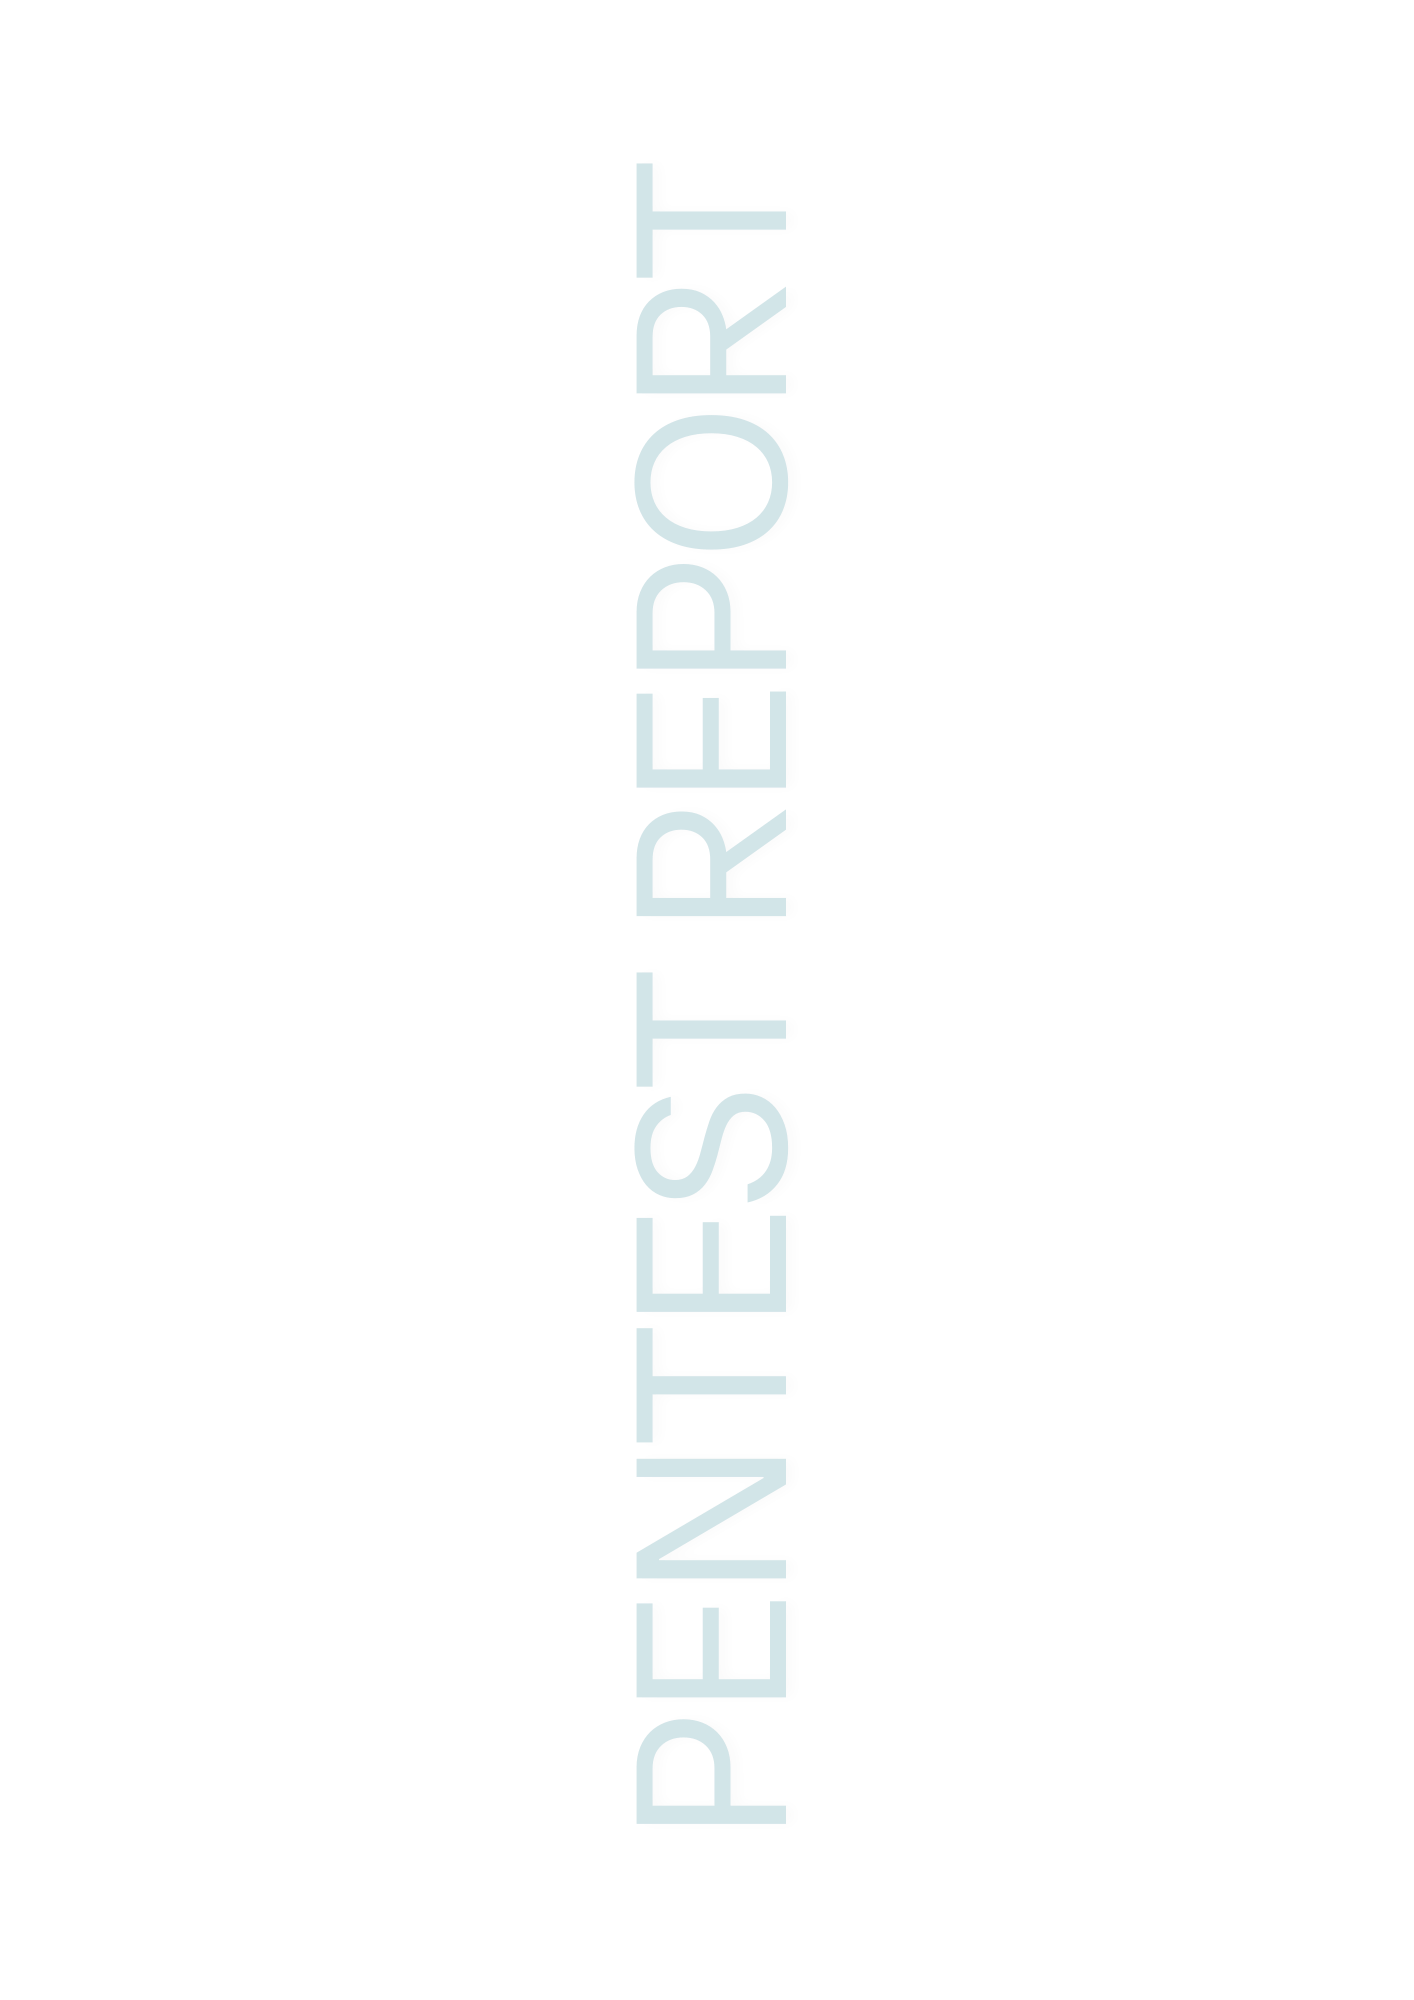
\includegraphics[height=\paperheight]{image_page_head.png}};
        \fill[headerblue] (current page.north west) rectangle ([yshift=-1cm]current page.north east);
    \end{tikzpicture}
}

% Footer
\fancyfoot[C]{
    \begin{tikzpicture}[remember picture, overlay]
        \fill[headerblue] (current page.south west) rectangle ([yshift=1cm]current page.south east);
        \node[anchor=south, yshift=0.25cm] at (current page.south) {\color{white}\bfseries\thepage};
    \end{tikzpicture}
}

\renewcommand{\headrulewidth}{0pt}
\renewcommand{\footrulewidth}{0pt}

% Title
\title{\Huge\textbf{\textcolor{headerblue}{Pentests Results}}}
\author{}
\date{}

% Adjust the style of sections (including \section*)
\usepackage{titlesec}
\titleformat{\section}[hang]{\Huge\bfseries\color{headerblue}}{}{0em}{}

% Hyperlink setup
\hypersetup{
    colorlinks=true,
    linkcolor=mylinkcolor,
    filecolor=magenta,
    urlcolor=myurlcolor,
}

\begin{document}

% Guard Page
\thispagestyle{empty}
\begin{tikzpicture}[remember picture, overlay]
    \node[anchor=north east, inner sep=0pt] at (current page.north east) {
\includegraphics[width=\paperwidth, height=\paperheight]{back_image.png}};
    \node[anchor=center, inner sep=0pt] at (current page.center) {
\includegraphics[height=0.5\paperheight]{centre.png}};
    \fill[white, opacity=0.5] (current page.south west) rectangle (current page.north east); % Blurry effect
\end{tikzpicture}
\newpage

% Table of Contents
\pagenumbering{Roman}
\tableofcontents
\newpage
\pagenumbering{arabic}

\maketitle
\thispagestyle{fancy}

% Adjust the vertical space after the title. Experiment with this value.
\vspace{-1em} 

% Add "Charts" title and charts on the same page
\afterpage{\aftergroup\restoregeometry % Restore geometry immediately after the page
    \thispagestyle{fancy} % Apply the fancy style to the blank page
    
    % Add "Charts" title and include both charts in a single figure environment
    \begin{figure}[htbp]
        \centering
        \caption*{\Huge\textbf{\textcolor{headerblue}{Charts}}} % Added Charts title
        \begin{subfigure}{\textwidth} % Full width for the subfigures
            \centering
            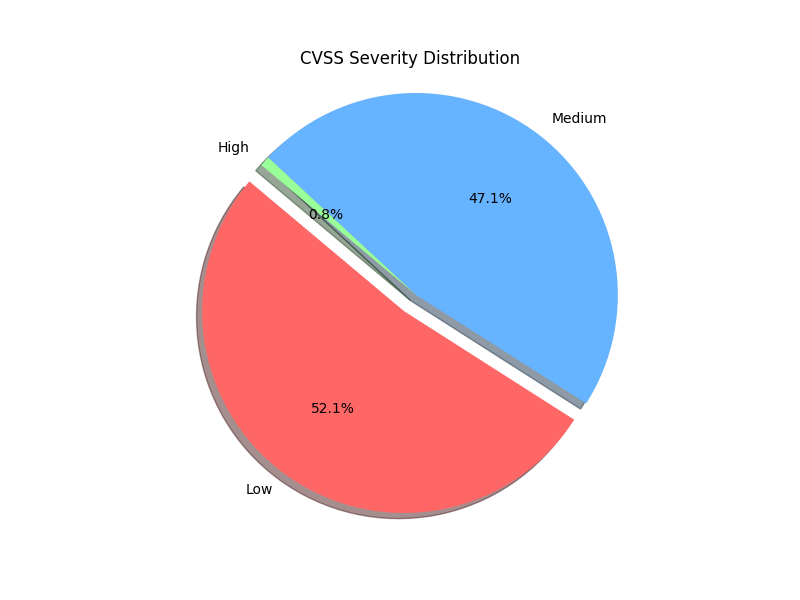
\includegraphics[width=0.9\linewidth]{alvo_pie_chart.png} % Adjust width of image as needed
            \caption{Figure 1: Pie Chart}
        \end{subfigure}
        
        \vspace{0.5cm} % Adjust vertical space between subfigures
        
        \begin{subfigure}{\textwidth} % Full width for the subfigures
            \centering
            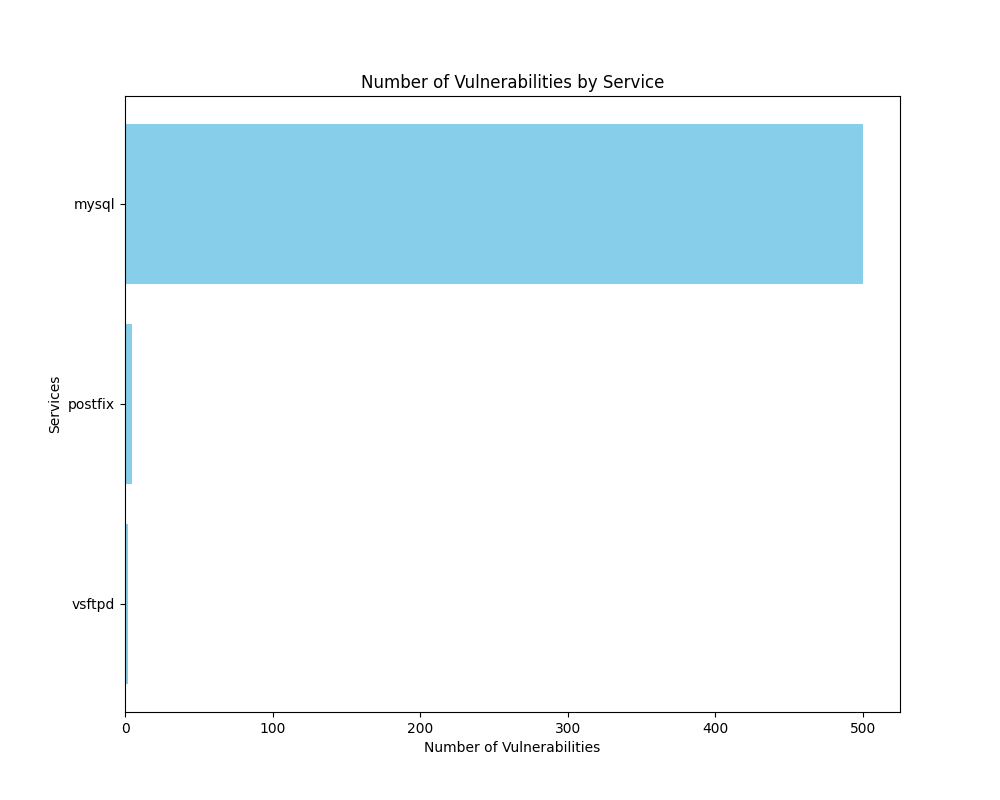
\includegraphics[width=0.9\linewidth]{alvo_bar_chart.png} % Adjust width of image as needed
            \caption{Figure 2: Bar Chart}
        \end{subfigure}
    \end{figure}
    \restoregeometry % Restore normal geometry settings
}

\begin{longtable}[]{@{}lll@{}}
\toprule
Company Name & First Name & Last Name\tabularnewline
\midrule
\endhead
Suse & John & Doe\tabularnewline
Manjaro & John & Doe\tabularnewline
KDE & John & Doe\tabularnewline
Gentoo & John & Doe\tabularnewline
Google & John & Doe\tabularnewline
Slackware & John & Doe\tabularnewline
Gnome & John & Doe\tabularnewline
Mozilla & John & Doe\tabularnewline
Thunderbird & John & Doe\tabularnewline
Bash & John & Doe\tabularnewline
JD & John & Doe\tabularnewline
Docker & John & Doe\tabularnewline
PostgreSQL & John & Doe\tabularnewline
Kali & John & Doe\tabularnewline
CVE-Search & John & Doe\tabularnewline
Metasploitable 2 & John & Doe\tabularnewline
Python & John & Doe\tabularnewline
VirtualBox & John & Doe\tabularnewline
VSCodium & John & Doe\tabularnewline
Apache & John & Doe\tabularnewline
HeidSql & John & Doe\tabularnewline
Wikipedia & John & Doe\tabularnewline
LXer & John & Doe\tabularnewline
ArchLinux & John & Doe\tabularnewline
Fedora & John & Doe\tabularnewline
Ubuntu & John & Doe\tabularnewline
Red Hat & John & Doe\tabularnewline
Debian & John & Doe\tabularnewline
Mint & John & Doe\tabularnewline
Rocky & John & Doe\tabularnewline
\bottomrule
\end{longtable}

\begin{longtable}[]{@{}lll@{}}
\toprule
Name & OS Name & OS SP\tabularnewline
\midrule
\endhead
victim & Linux & 8.04\tabularnewline
\bottomrule
\end{longtable}

\begin{longtable}[]{@{}ll@{}}
\toprule
CVE & Critical Severity\tabularnewline
\midrule
\endhead
\protect\hyperlink{CVE-2011-2523}{CVE-CVE-2011-2523} &
{10.0}\tabularnewline
\protect\hyperlink{CVE-2008-0122}{CVE-CVE-2008-0122} &
{10.0}\tabularnewline
\protect\hyperlink{CVE-2003-0789}{CVE-CVE-2003-0789} &
{10.0}\tabularnewline
\protect\hyperlink{CVE-2005-2700}{CVE-CVE-2005-2700} &
{10.0}\tabularnewline
\protect\hyperlink{CVE-2010-0425}{CVE-CVE-2010-0425} &
{10.0}\tabularnewline
\protect\hyperlink{CVE-2013-1902}{CVE-CVE-2013-1902} &
{10.0}\tabularnewline
\protect\hyperlink{CVE-2013-1903}{CVE-CVE-2013-1903} &
{10.0}\tabularnewline
\protect\hyperlink{CVE-2016-7048}{CVE-CVE-2016-7048} &
{9.3}\tabularnewline
\bottomrule
\end{longtable}

\hypertarget{details}{%
\section{Details}\label{details}}

\hypertarget{cve-2011-2523}{%
\subsection{CVE-2011-2523}\label{cve-2011-2523}}

!--\textgreater{} CVE for
cpe:2.3:a:vsftpd\_project:vsftpd:2.3.4:\emph{:}:\emph{:}:\emph{:}:*
Summary: vsftpd 2.3.4 downloaded between 20110630 and 20110703 contains
a backdoor which opens a shell on port 6200/tcp.

\textbf{\textcolor{red}{CVSS: 10.0}}

\hypertarget{cve-2021-3618}{%
\subsection{CVE-2021-3618}\label{cve-2021-3618}}

!--\textgreater{} CVE for
cpe:2.3:a:vsftpd\_project:vsftpd:2.3.4:\emph{:}:\emph{:}:\emph{:}:*
Summary: ALPACA is an application layer protocol content confusion
attack, exploiting TLS servers implementing different protocols but
using compatible certificates, such as multi-domain or wildcard
certificates. A MiTM attacker having access to victim's traffic at the
TCP/IP layer can redirect traffic from one subdomain to another,
resulting in a valid TLS session. This breaks the authentication of TLS
and cross-protocol attacks may be possible where the behavior of one
protocol service may compromise the other at the application layer.

\textbf{\textcolor{red}{CVSS: 5.8}}

\hypertarget{cve-2010-4478}{%
\subsection{CVE-2010-4478}\label{cve-2010-4478}}

!--\textgreater{} CVE for
cpe:2.3:a:openbsd:openssh:4.7p1:\emph{:}:\emph{:}:\emph{:}:* Summary:
OpenSSH 5.6 and earlier, when J-PAKE is enabled, does not properly
validate the public parameters in the J-PAKE protocol, which allows
remote attackers to bypass the need for knowledge of the shared secret,
and successfully authenticate, by sending crafted values in each round
of the protocol, a related issue to CVE-2010-4252.

\textbf{\textcolor{red}{CVSS: 7.5}}

\hypertarget{cve-2010-4755}{%
\subsection{CVE-2010-4755}\label{cve-2010-4755}}

!--\textgreater{} CVE for
cpe:2.3:a:openbsd:openssh:4.7p1:\emph{:}:\emph{:}:\emph{:}:* Summary:
The (1) remote\_glob function in sftp-glob.c and the (2) process\_put
function in sftp.c in OpenSSH 5.8 and earlier, as used in FreeBSD 7.3
and 8.1, NetBSD 5.0.2, OpenBSD 4.7, and other products, allow remote
authenticated users to cause a denial of service (CPU and memory
consumption) via crafted glob expressions that do not match any
pathnames, as demonstrated by glob expressions in SSH\_FXP\_STAT
requests to an sftp daemon, a different vulnerability than
CVE-2010-2632.

\textbf{\textcolor{red}{CVSS: 4.0}}

\hypertarget{cve-2008-5161}{%
\subsection{CVE-2008-5161}\label{cve-2008-5161}}

!--\textgreater{} CVE for
cpe:2.3:a:openbsd:openssh:4.7p1:\emph{:}:\emph{:}:\emph{:}:* Summary:
Error handling in the SSH protocol in (1) SSH Tectia Client and Server
and Connector 4.0 through 4.4.11, 5.0 through 5.2.4, and 5.3 through
5.3.8; Client and Server and ConnectSecure 6.0 through 6.0.4; Server for
Linux on IBM System z 6.0.4; Server for IBM z/OS 5.5.1 and earlier,
6.0.0, and 6.0.1; and Client 4.0-J through 4.3.3-J and 4.0-K through
4.3.10-K; and (2) OpenSSH 4.7p1 and possibly other versions, when using
a block cipher algorithm in Cipher Block Chaining (CBC) mode, makes it
easier for remote attackers to recover certain plaintext data from an
arbitrary block of ciphertext in an SSH session via unknown vectors.

\textbf{\textcolor{red}{CVSS: 2.6}}

\hypertarget{cve-2004-0998}{%
\subsection{CVE-2004-0998}\label{cve-2004-0998}}

!--\textgreater{} CVE for
cpe:2.3:a:telnetd:telnetd:0.17.25:\emph{:}:\emph{:}:\emph{:}:* Summary:
Format string vulnerability in telnetd-ssl 0.17 and earlier allows
remote attackers to execute arbitrary code.

\textbf{\textcolor{red}{CVSS: 7.5}}

\hypertarget{cve-2011-0411}{%
\subsection{CVE-2011-0411}\label{cve-2011-0411}}

!--\textgreater{} CVE for
cpe:2.3:a:postfix:postfix:2.4:\emph{:}:\emph{:}:\emph{:}:* Summary: The
STARTTLS implementation in Postfix 2.4.x before 2.4.16, 2.5.x before
2.5.12, 2.6.x before 2.6.9, and 2.7.x before 2.7.3 does not properly
restrict I/O buffering, which allows man-in-the-middle attackers to
insert commands into encrypted SMTP sessions by sending a cleartext
command that is processed after TLS is in place, related to a
``plaintext command injection'' attack.

\textbf{\textcolor{red}{CVSS: 6.8}}

\hypertarget{cve-2011-1720}{%
\subsection{CVE-2011-1720}\label{cve-2011-1720}}

!--\textgreater{} CVE for
cpe:2.3:a:postfix:postfix:2.4:\emph{:}:\emph{:}:\emph{:}:* Summary: The
SMTP server in Postfix before 2.5.13, 2.6.x before 2.6.10, 2.7.x before
2.7.4, and 2.8.x before 2.8.3, when certain Cyrus SASL authentication
methods are enabled, does not create a new server handle after client
authentication fails, which allows remote attackers to cause a denial of
service (heap memory corruption and daemon crash) or possibly execute
arbitrary code via an invalid AUTH command with one method followed by
an AUTH command with a different method.

\textbf{\textcolor{red}{CVSS: 6.8}}

\hypertarget{cve-2017-10140}{%
\subsection{CVE-2017-10140}\label{cve-2017-10140}}

!--\textgreater{} CVE for
cpe:2.3:a:postfix:postfix:2.4:\emph{:}:\emph{:}:\emph{:}:* Summary:
Postfix before 2.11.10, 3.0.x before 3.0.10, 3.1.x before 3.1.6, and
3.2.x before 3.2.2 might allow local users to gain privileges by
leveraging undocumented functionality in Berkeley DB 2.x and later,
related to reading settings from DB\_CONFIG in the current directory.

\textbf{\textcolor{red}{CVSS: 4.6}}

\hypertarget{cve-2008-3889}{%
\subsection{CVE-2008-3889}\label{cve-2008-3889}}

!--\textgreater{} CVE for
cpe:2.3:a:postfix:postfix:2.4:\emph{:}:\emph{:}:\emph{:}:* Summary:
Postfix 2.4 before 2.4.9, 2.5 before 2.5.5, and 2.6 before 2.6-20080902,
when used with the Linux 2.6 kernel, leaks epoll file descriptors during
execution of ``non-Postfix'' commands, which allows local users to cause
a denial of service (application slowdown or exit) via a crafted
command, as demonstrated by a command in a .forward file.

\textbf{\textcolor{red}{CVSS: 2.1}}

\hypertarget{cve-2023-51764}{%
\subsection{CVE-2023-51764}\label{cve-2023-51764}}

!--\textgreater{} CVE for
cpe:2.3:a:postfix:postfix:2.4:\emph{:}:\emph{:}:\emph{:}:* Summary:
Postfix through 3.8.5 allows SMTP smuggling unless configured with
smtpd\_data\_restrictions=reject\_unauth\_pipelining and
smtpd\_discard\_ehlo\_keywords=chunking (or certain other options that
exist in recent versions). Remote attackers can use a published
exploitation technique to inject e-mail messages with a spoofed MAIL
FROM address, allowing bypass of an SPF protection mechanism. This
occurs because Postfix supports . but some other popular e-mail servers
do not. To prevent attack variants (by always disallowing without ), a
different solution is required, such as the
smtpd\_forbid\_bare\_newline=yes option with a Postfix minimum version
of 3.5.23, 3.6.13, 3.7.9, 3.8.4, or 3.9.

\textbf{\textcolor{red}{CVSS: N/A}}

\hypertarget{cve-2008-0122}{%
\subsection{CVE-2008-0122}\label{cve-2008-0122}}

!--\textgreater{} CVE for
cpe:2.3:a:isc:bind:9.0:\emph{:}:\emph{:}:\emph{:}:* Summary: Off-by-one
error in the inet\_network function in libbind in ISC BIND 9.4.2 and
earlier, as used in libc in FreeBSD 6.2 through 7.0-PRERELEASE, allows
context-dependent attackers to cause a denial of service (crash) and
possibly execute arbitrary code via crafted input that triggers memory
corruption.

\textbf{\textcolor{red}{CVSS: 10.0}}

\hypertarget{cve-2012-1667}{%
\subsection{CVE-2012-1667}\label{cve-2012-1667}}

!--\textgreater{} CVE for
cpe:2.3:a:isc:bind:9.0:\emph{:}:\emph{:}:\emph{:}:* Summary: ISC BIND
9.x before 9.7.6-P1, 9.8.x before 9.8.3-P1, 9.9.x before 9.9.1-P1, and
9.4-ESV and 9.6-ESV before 9.6-ESV-R7-P1 does not properly handle
resource records with a zero-length RDATA section, which allows remote
DNS servers to cause a denial of service (daemon crash or data
corruption) or obtain sensitive information from process memory via a
crafted record.

\textbf{\textcolor{red}{CVSS: 8.5}}

\hypertarget{cve-2012-4244}{%
\subsection{CVE-2012-4244}\label{cve-2012-4244}}

!--\textgreater{} CVE for
cpe:2.3:a:isc:bind:9.0:\emph{:}:\emph{:}:\emph{:}:* Summary: ISC BIND
9.x before 9.7.6-P3, 9.8.x before 9.8.3-P3, 9.9.x before 9.9.1-P3, and
9.4-ESV and 9.6-ESV before 9.6-ESV-R7-P3 allows remote attackers to
cause a denial of service (assertion failure and named daemon exit) via
a query for a long resource record.

\textbf{\textcolor{red}{CVSS: 7.8}}

\hypertarget{cve-2012-5166}{%
\subsection{CVE-2012-5166}\label{cve-2012-5166}}

!--\textgreater{} CVE for
cpe:2.3:a:isc:bind:9.0:\emph{:}:\emph{:}:\emph{:}:* Summary: ISC BIND
9.x before 9.7.6-P4, 9.8.x before 9.8.3-P4, 9.9.x before 9.9.1-P4, and
9.4-ESV and 9.6-ESV before 9.6-ESV-R7-P4 allows remote attackers to
cause a denial of service (named daemon hang) via unspecified
combinations of resource records.

\textbf{\textcolor{red}{CVSS: 7.8}}

\hypertarget{cve-2014-8500}{%
\subsection{CVE-2014-8500}\label{cve-2014-8500}}

!--\textgreater{} CVE for
cpe:2.3:a:isc:bind:9.0:\emph{:}:\emph{:}:\emph{:}:* Summary: ISC BIND
9.0.x through 9.8.x, 9.9.0 through 9.9.6, and 9.10.0 through 9.10.1 does
not limit delegation chaining, which allows remote attackers to cause a
denial of service (memory consumption and named crash) via a large or
infinite number of referrals.

\textbf{\textcolor{red}{CVSS: 7.8}}

\hypertarget{cve-2015-5477}{%
\subsection{CVE-2015-5477}\label{cve-2015-5477}}

!--\textgreater{} CVE for
cpe:2.3:a:isc:bind:9.0:\emph{:}:\emph{:}:\emph{:}:* Summary: named in
ISC BIND 9.x before 9.9.7-P2 and 9.10.x before 9.10.2-P3 allows remote
attackers to cause a denial of service (REQUIRE assertion failure and
daemon exit) via TKEY queries.

\textbf{\textcolor{red}{CVSS: 7.8}}

\hypertarget{cve-2015-5722}{%
\subsection{CVE-2015-5722}\label{cve-2015-5722}}

!--\textgreater{} CVE for
cpe:2.3:a:isc:bind:9.0:\emph{:}:\emph{:}:\emph{:}:* Summary: buffer.c in
named in ISC BIND 9.x before 9.9.7-P3 and 9.10.x before 9.10.2-P4 allows
remote attackers to cause a denial of service (assertion failure and
daemon exit) by creating a zone containing a malformed DNSSEC key and
issuing a query for a name in that zone.

\textbf{\textcolor{red}{CVSS: 7.8}}

\hypertarget{cve-2016-2776}{%
\subsection{CVE-2016-2776}\label{cve-2016-2776}}

!--\textgreater{} CVE for
cpe:2.3:a:isc:bind:9.0:\emph{:}:\emph{:}:\emph{:}:* Summary: buffer.c in
named in ISC BIND 9 before 9.9.9-P3, 9.10.x before 9.10.4-P3, and 9.11.x
before 9.11.0rc3 does not properly construct responses, which allows
remote attackers to cause a denial of service (assertion failure and
daemon exit) via a crafted query.

\textbf{\textcolor{red}{CVSS: 7.8}}

\hypertarget{cve-2010-0382}{%
\subsection{CVE-2010-0382}\label{cve-2010-0382}}

!--\textgreater{} CVE for
cpe:2.3:a:isc:bind:9.0:\emph{:}:\emph{:}:\emph{:}:* Summary: ISC BIND
9.0.x through 9.3.x, 9.4 before 9.4.3-P5, 9.5 before 9.5.2-P2, 9.6
before 9.6.1-P3, and 9.7.0 beta handles out-of-bailiwick data
accompanying a secure response without re-fetching from the original
source, which allows remote attackers to have an unspecified impact via
a crafted response, aka Bug 20819. NOTE: this vulnerability exists
because of a regression during the fix for CVE-2009-4022.

\textbf{\textcolor{red}{CVSS: 7.6}}

\hypertarget{cve-2015-8461}{%
\subsection{CVE-2015-8461}\label{cve-2015-8461}}

!--\textgreater{} CVE for
cpe:2.3:a:isc:bind:9.0:\emph{:}:\emph{:}:\emph{:}:* Summary: Race
condition in resolver.c in named in ISC BIND 9.9.8 before 9.9.8-P2 and
9.10.3 before 9.10.3-P2 allows remote attackers to cause a denial of
service (INSIST assertion failure and daemon exit) via unspecified
vectors.

\textbf{\textcolor{red}{CVSS: 7.1}}

\hypertarget{cve-2015-5986}{%
\subsection{CVE-2015-5986}\label{cve-2015-5986}}

!--\textgreater{} CVE for
cpe:2.3:a:isc:bind:9.0:\emph{:}:\emph{:}:\emph{:}:* Summary:
openpgpkey\_61.c in named in ISC BIND 9.9.7 before 9.9.7-P3 and 9.10.x
before 9.10.2-P4 allows remote attackers to cause a denial of service
(REQUIRE assertion failure and daemon exit) via a crafted DNS response.

\textbf{\textcolor{red}{CVSS: 7.1}}

\hypertarget{cve-2009-0025}{%
\subsection{CVE-2009-0025}\label{cve-2009-0025}}

!--\textgreater{} CVE for
cpe:2.3:a:isc:bind:9.0:\emph{:}:\emph{:}:\emph{:}:* Summary: BIND 9.6.0,
9.5.1, 9.5.0, 9.4.3, and earlier does not properly check the return
value from the OpenSSL DSA\_verify function, which allows remote
attackers to bypass validation of the certificate chain via a malformed
SSL/TLS signature, a similar vulnerability to CVE-2008-5077.

\textbf{\textcolor{red}{CVSS: 6.8}}

\hypertarget{cve-2015-8704}{%
\subsection{CVE-2015-8704}\label{cve-2015-8704}}

!--\textgreater{} CVE for
cpe:2.3:a:isc:bind:9.0:\emph{:}:\emph{:}:\emph{:}:* Summary: apl\_42.c
in ISC BIND 9.x before 9.9.8-P3, 9.9.x, and 9.10.x before 9.10.3-P3
allows remote authenticated users to cause a denial of service (INSIST
assertion failure and daemon exit) via a malformed Address Prefix List
(APL) record.

\textbf{\textcolor{red}{CVSS: 6.8}}

\hypertarget{cve-2015-8705}{%
\subsection{CVE-2015-8705}\label{cve-2015-8705}}

!--\textgreater{} CVE for
cpe:2.3:a:isc:bind:9.0:\emph{:}:\emph{:}:\emph{:}:* Summary: buffer.c in
named in ISC BIND 9.10.x before 9.10.3-P3, when debug logging is
enabled, allows remote attackers to cause a denial of service (REQUIRE
assertion failure and daemon exit, or daemon crash) or possibly have
unspecified other impact via (1) OPT data or (2) an ECS option.

\textbf{\textcolor{red}{CVSS: 6.6}}

\hypertarget{cve-2010-3614}{%
\subsection{CVE-2010-3614}\label{cve-2010-3614}}

!--\textgreater{} CVE for
cpe:2.3:a:isc:bind:9.0:\emph{:}:\emph{:}:\emph{:}:* Summary: named in
ISC BIND 9.x before 9.6.2-P3, 9.7.x before 9.7.2-P3, 9.4-ESV before
9.4-ESV-R4, and 9.6-ESV before 9.6-ESV-R3 does not properly determine
the security status of an NS RRset during a DNSKEY algorithm rollover,
which might allow remote attackers to cause a denial of service (DNSSEC
validation error) by triggering a rollover.

\textbf{\textcolor{red}{CVSS: 6.4}}

\hypertarget{cve-2002-0400}{%
\subsection{CVE-2002-0400}\label{cve-2002-0400}}

!--\textgreater{} CVE for
cpe:2.3:a:isc:bind:9.0:\emph{:}:\emph{:}:\emph{:}:* Summary: ISC BIND 9
before 9.2.1 allows remote attackers to cause a denial of service
(shutdown) via a malformed DNS packet that triggers an error condition
that is not properly handled when the rdataset parameter to the
dns\_message\_findtype() function in message.c is not NULL, aka
DoS\_findtype.

\textbf{\textcolor{red}{CVSS: 5.0}}

\hypertarget{cve-2006-2073}{%
\subsection{CVE-2006-2073}\label{cve-2006-2073}}

!--\textgreater{} CVE for
cpe:2.3:a:isc:bind:9.0:\emph{:}:\emph{:}:\emph{:}:* Summary: Unspecified
vulnerability in ISC BIND allows remote attackers to cause a denial of
service via a crafted DNS message with a ``broken'' TSIG, as
demonstrated by the OUSPG PROTOS DNS test suite.

\textbf{\textcolor{red}{CVSS: 5.0}}

\hypertarget{cve-2011-1910}{%
\subsection{CVE-2011-1910}\label{cve-2011-1910}}

!--\textgreater{} CVE for
cpe:2.3:a:isc:bind:9.0:\emph{:}:\emph{:}:\emph{:}:* Summary: Off-by-one
error in named in ISC BIND 9.x before 9.7.3-P1, 9.8.x before 9.8.0-P2,
9.4-ESV before 9.4-ESV-R4-P1, and 9.6-ESV before 9.6-ESV-R4-P1 allows
remote DNS servers to cause a denial of service (assertion failure and
daemon exit) via a negative response containing large RRSIG RRsets.

\textbf{\textcolor{red}{CVSS: 5.0}}

\hypertarget{cve-2011-4313}{%
\subsection{CVE-2011-4313}\label{cve-2011-4313}}

!--\textgreater{} CVE for
cpe:2.3:a:isc:bind:9.0:\emph{:}:\emph{:}:\emph{:}:* Summary: query.c in
ISC BIND 9.0.x through 9.6.x, 9.4-ESV through 9.4-ESV-R5, 9.6-ESV
through 9.6-ESV-R5, 9.7.0 through 9.7.4, 9.8.0 through 9.8.1, and
9.9.0a1 through 9.9.0b1 allows remote attackers to cause a denial of
service (assertion failure and named exit) via unknown vectors related
to recursive DNS queries, error logging, and the caching of an invalid
record by the resolver.

\textbf{\textcolor{red}{CVSS: 5.0}}

\hypertarget{cve-2012-1033}{%
\subsection{CVE-2012-1033}\label{cve-2012-1033}}

!--\textgreater{} CVE for
cpe:2.3:a:isc:bind:9.0:\emph{:}:\emph{:}:\emph{:}:* Summary: The
resolver in ISC BIND 9 through 9.8.1-P1 overwrites cached server names
and TTL values in NS records during the processing of a response to an A
record query, which allows remote attackers to trigger continued
resolvability of revoked domain names via a ``ghost domain names''
attack.

\textbf{\textcolor{red}{CVSS: 5.0}}

\hypertarget{cve-2015-8000}{%
\subsection{CVE-2015-8000}\label{cve-2015-8000}}

!--\textgreater{} CVE for
cpe:2.3:a:isc:bind:9.0:\emph{:}:\emph{:}:\emph{:}:* Summary: db.c in
named in ISC BIND 9.x before 9.9.8-P2 and 9.10.x before 9.10.3-P2 allows
remote attackers to cause a denial of service (REQUIRE assertion failure
and daemon exit) via a malformed class attribute.

\textbf{\textcolor{red}{CVSS: 5.0}}

\hypertarget{cve-2016-9444}{%
\subsection{CVE-2016-9444}\label{cve-2016-9444}}

!--\textgreater{} CVE for
cpe:2.3:a:isc:bind:9.0:\emph{:}:\emph{:}:\emph{:}:* Summary: named in
ISC BIND 9.x before 9.9.9-P5, 9.10.x before 9.10.4-P5, and 9.11.x before
9.11.0-P2 allows remote attackers to cause a denial of service
(assertion failure and daemon exit) via a crafted DS resource record in
an answer.

\textbf{\textcolor{red}{CVSS: 5.0}}

\hypertarget{cve-2006-4095}{%
\subsection{CVE-2006-4095}\label{cve-2006-4095}}

!--\textgreater{} CVE for
cpe:2.3:a:isc:bind:9.0:\emph{:}:\emph{:}:\emph{:}:* Summary: BIND before
9.2.6-P1 and 9.3.x before 9.3.2-P1 allows remote attackers to cause a
denial of service (crash) via certain SIG queries, which cause an
assertion failure when multiple RRsets are returned.

\textbf{\textcolor{red}{CVSS: 5.0}}

\hypertarget{cve-2009-0265}{%
\subsection{CVE-2009-0265}\label{cve-2009-0265}}

!--\textgreater{} CVE for
cpe:2.3:a:isc:bind:9.0:\emph{:}:\emph{:}:\emph{:}:* Summary: Internet
Systems Consortium (ISC) BIND 9.6.0 and earlier does not properly check
the return value from the OpenSSL EVP\_VerifyFinal function, which
allows remote attackers to bypass validation of the certificate chain
via a malformed SSL/TLS signature, a similar vulnerability to
CVE-2008-5077 and CVE-2009-0025.

\textbf{\textcolor{red}{CVSS: 5.0}}

\hypertarget{cve-2016-9131}{%
\subsection{CVE-2016-9131}\label{cve-2016-9131}}

!--\textgreater{} CVE for
cpe:2.3:a:isc:bind:9.0:\emph{:}:\emph{:}:\emph{:}:* Summary: named in
ISC BIND 9.x before 9.9.9-P5, 9.10.x before 9.10.4-P5, and 9.11.x before
9.11.0-P2 allows remote attackers to cause a denial of service
(assertion failure and daemon exit) via a malformed response to an RTYPE
ANY query.

\textbf{\textcolor{red}{CVSS: 5.0}}

\hypertarget{cve-2001-0497}{%
\subsection{CVE-2001-0497}\label{cve-2001-0497}}

!--\textgreater{} CVE for
cpe:2.3:a:isc:bind:9.0:\emph{:}:\emph{:}:\emph{:}:* Summary: dnskeygen
in BIND 8.2.4 and earlier, and dnssec-keygen in BIND 9.1.2 and earlier,
set insecure permissions for a HMAC-MD5 shared secret key file used for
DNS Transactional Signatures (TSIG), which allows attackers to obtain
the keys and perform dynamic DNS updates.

\textbf{\textcolor{red}{CVSS: 4.6}}

\hypertarget{cve-2007-0494}{%
\subsection{CVE-2007-0494}\label{cve-2007-0494}}

!--\textgreater{} CVE for
cpe:2.3:a:isc:bind:9.0:\emph{:}:\emph{:}:\emph{:}:\emph{ Summary: ISC
BIND 9.0.x, 9.1.x, 9.2.0 up to 9.2.7, 9.3.0 up to 9.3.3, 9.4.0a1 up to
9.4.0a6, 9.4.0b1 up to 9.4.0b4, 9.4.0rc1, and 9.5.0a1 (Bind Forum only)
allows remote attackers to cause a denial of service (exit) via a type }
(ANY) DNS query response that contains multiple RRsets, which triggers
an assertion error, aka the ``DNSSEC Validation'' vulnerability.

\textbf{\textcolor{red}{CVSS: 4.3}}

\hypertarget{cve-2007-2926}{%
\subsection{CVE-2007-2926}\label{cve-2007-2926}}

!--\textgreater{} CVE for
cpe:2.3:a:isc:bind:9.0:\emph{:}:\emph{:}:\emph{:}:* Summary: ISC BIND 9
through 9.5.0a5 uses a weak random number generator during generation of
DNS query ids when answering resolver questions or sending NOTIFY
messages to slave name servers, which makes it easier for remote
attackers to guess the next query id and perform DNS cache poisoning.

\textbf{\textcolor{red}{CVSS: 4.3}}

\hypertarget{cve-2010-0097}{%
\subsection{CVE-2010-0097}\label{cve-2010-0097}}

!--\textgreater{} CVE for
cpe:2.3:a:isc:bind:9.0:\emph{:}:\emph{:}:\emph{:}:* Summary: ISC BIND
9.0.x through 9.3.x, 9.4 before 9.4.3-P5, 9.5 before 9.5.2-P2, 9.6
before 9.6.1-P3, and 9.7.0 beta does not properly validate DNSSEC (1)
NSEC and (2) NSEC3 records, which allows remote attackers to add the
Authenticated Data (AD) flag to a forged NXDOMAIN response for an
existing domain.

\textbf{\textcolor{red}{CVSS: 4.3}}

\hypertarget{cve-2010-3762}{%
\subsection{CVE-2010-3762}\label{cve-2010-3762}}

!--\textgreater{} CVE for
cpe:2.3:a:isc:bind:9.0:\emph{:}:\emph{:}:\emph{:}:* Summary: ISC BIND
before 9.7.2-P2, when DNSSEC validation is enabled, does not properly
handle certain bad signatures if multiple trust anchors exist for a
single zone, which allows remote attackers to cause a denial of service
(daemon crash) via a DNS query.

\textbf{\textcolor{red}{CVSS: 4.3}}

\hypertarget{cve-2016-2775}{%
\subsection{CVE-2016-2775}\label{cve-2016-2775}}

!--\textgreater{} CVE for
cpe:2.3:a:isc:bind:9.0:\emph{:}:\emph{:}:\emph{:}:* Summary: ISC BIND
9.x before 9.9.9-P2, 9.10.x before 9.10.4-P2, and 9.11.x before
9.11.0b2, when lwresd or the named lwres option is enabled, allows
remote attackers to cause a denial of service (daemon crash) via a long
request that uses the lightweight resolver protocol.

\textbf{\textcolor{red}{CVSS: 4.3}}

\hypertarget{cve-2010-0290}{%
\subsection{CVE-2010-0290}\label{cve-2010-0290}}

!--\textgreater{} CVE for
cpe:2.3:a:isc:bind:9.0:\emph{:}:\emph{:}:\emph{:}:* Summary: Unspecified
vulnerability in ISC BIND 9.0.x through 9.3.x, 9.4 before 9.4.3-P5, 9.5
before 9.5.2-P2, 9.6 before 9.6.1-P3, and 9.7.0 beta, with DNSSEC
validation enabled and checking disabled (CD), allows remote attackers
to conduct DNS cache poisoning attacks by receiving a recursive client
query and sending a response that contains (1) CNAME or (2) DNAME
records, which do not have the intended validation before caching, aka
Bug 20737. NOTE: this vulnerability exists because of an incomplete fix
for CVE-2009-4022.

\textbf{\textcolor{red}{CVSS: 4.0}}

\hypertarget{cve-2016-6170}{%
\subsection{CVE-2016-6170}\label{cve-2016-6170}}

!--\textgreater{} CVE for
cpe:2.3:a:isc:bind:9.0:\emph{:}:\emph{:}:\emph{:}:* Summary: ISC BIND
through 9.9.9-P1, 9.10.x through 9.10.4-P1, and 9.11.x through 9.11.0b1
allows primary DNS servers to cause a denial of service (secondary DNS
server crash) via a large AXFR response, and possibly allows IXFR
servers to cause a denial of service (IXFR client crash) via a large
IXFR response and allows remote authenticated users to cause a denial of
service (primary DNS server crash) via a large UPDATE message.

\textbf{\textcolor{red}{CVSS: 4.0}}

\hypertarget{cve-2018-5741}{%
\subsection{CVE-2018-5741}\label{cve-2018-5741}}

!--\textgreater{} CVE for
cpe:2.3:a:isc:bind:9.0:\emph{:}:\emph{:}:\emph{:}:* Summary: To provide
fine-grained controls over the ability to use Dynamic DNS (DDNS) to
update records in a zone, BIND 9 provides a feature called
update-policy. Various rules can be configured to limit the types of
updates that can be performed by a client, depending on the key used
when sending the update request. Unfortunately, some rule types were not
initially documented, and when documentation for them was added to the
Administrator Reference Manual (ARM) in change \#3112, the language that
was added to the ARM at that time incorrectly described the behavior of
two rule types, krb5-subdomain and ms-subdomain. This incorrect
documentation could mislead operators into believing that policies they
had configured were more restrictive than they actually were. This
affects BIND versions prior to BIND 9.11.5 and BIND 9.12.3.

\textbf{\textcolor{red}{CVSS: 4.0}}

\hypertarget{cve-2009-4022}{%
\subsection{CVE-2009-4022}\label{cve-2009-4022}}

!--\textgreater{} CVE for
cpe:2.3:a:isc:bind:9.0:\emph{:}:\emph{:}:\emph{:}:* Summary: Unspecified
vulnerability in ISC BIND 9.0.x through 9.3.x, 9.4 before 9.4.3-P4, 9.5
before 9.5.2-P1, 9.6 before 9.6.1-P2, and 9.7 beta before 9.7.0b3, with
DNSSEC validation enabled and checking disabled (CD), allows remote
attackers to conduct DNS cache poisoning attacks by receiving a
recursive client query and sending a response that contains an
Additional section with crafted data, which is not properly handled when
the response is processed ``at the same time as requesting DNSSEC
records (DO),'' aka Bug 20438.

\textbf{\textcolor{red}{CVSS: 2.6}}

\hypertarget{cve-2003-0789}{%
\subsection{CVE-2003-0789}\label{cve-2003-0789}}

!--\textgreater{} CVE for
cpe:2.3:a:apache:http\_server:2.0.36:\emph{:}:\emph{:}:\emph{:}:*
Summary: mod\_cgid in Apache before 2.0.48, when using a threaded MPM,
does not properly handle CGI redirect paths, which could cause Apache to
send the output of a CGI program to the wrong client.

\textbf{\textcolor{red}{CVSS: 10.0}}

\hypertarget{cve-2005-2700}{%
\subsection{CVE-2005-2700}\label{cve-2005-2700}}

!--\textgreater{} CVE for
cpe:2.3:a:apache:http\_server:2.0.36:\emph{:}:\emph{:}:\emph{:}:*
Summary: ssl\_engine\_kernel.c in mod\_ssl before 2.8.24, when using
``SSLVerifyClient optional'' in the global virtual host configuration,
does not properly enforce ``SSLVerifyClient require'' in a per-location
context, which allows remote attackers to bypass intended access
restrictions.

\textbf{\textcolor{red}{CVSS: 10.0}}

\hypertarget{cve-2010-0425}{%
\subsection{CVE-2010-0425}\label{cve-2010-0425}}

!--\textgreater{} CVE for
cpe:2.3:a:apache:http\_server:2.0.36:\emph{:}:\emph{:}:\emph{:}:*
Summary: modules/arch/win32/mod\_isapi.c in mod\_isapi in the Apache
HTTP Server 2.0.37 through 2.0.63, 2.2.0 through 2.2.14, and 2.3.x
before 2.3.7, when running on Windows, does not ensure that request
processing is complete before calling isapi\_unload for an ISAPI .dll
module, which allows remote attackers to execute arbitrary code via
unspecified vectors related to a crafted request, a reset packet, and
``orphaned callback pointers.''

\textbf{\textcolor{red}{CVSS: 10.0}}

\hypertarget{cve-2011-3192}{%
\subsection{CVE-2011-3192}\label{cve-2011-3192}}

!--\textgreater{} CVE for
cpe:2.3:a:apache:http\_server:2.0.36:\emph{:}:\emph{:}:\emph{:}:*
Summary: The byterange filter in the Apache HTTP Server 1.3.x, 2.0.x
through 2.0.64, and 2.2.x through 2.2.19 allows remote attackers to
cause a denial of service (memory and CPU consumption) via a Range
header that expresses multiple overlapping ranges, as exploited in the
wild in August 2011, a different vulnerability than CVE-2007-0086.

\textbf{\textcolor{red}{CVSS: 7.8}}

\hypertarget{cve-2002-0392}{%
\subsection{CVE-2002-0392}\label{cve-2002-0392}}

!--\textgreater{} CVE for
cpe:2.3:a:apache:http\_server:2.0.36:\emph{:}:\emph{:}:\emph{:}:*
Summary: Apache 1.3 through 1.3.24, and Apache 2.0 through 2.0.36,
allows remote attackers to cause a denial of service and possibly
execute arbitrary code via a chunk-encoded HTTP request that causes
Apache to use an incorrect size.

\textbf{\textcolor{red}{CVSS: 7.5}}

\hypertarget{cve-2002-0661}{%
\subsection{CVE-2002-0661}\label{cve-2002-0661}}

!--\textgreater{} CVE for
cpe:2.3:a:apache:http\_server:2.0.36:\emph{:}:\emph{:}:\emph{:}:*
Summary: Directory traversal vulnerability in Apache 2.0 through 2.0.39
on Windows, OS2, and Netware allows remote attackers to read arbitrary
files and execute commands via .. (dot dot) sequences containing
~(backslash) characters.

\textbf{\textcolor{red}{CVSS: 7.5}}

\hypertarget{cve-2003-0016}{%
\subsection{CVE-2003-0016}\label{cve-2003-0016}}

!--\textgreater{} CVE for
cpe:2.3:a:apache:http\_server:2.0.36:\emph{:}:\emph{:}:\emph{:}:*
Summary: Apache before 2.0.44, when running on unpatched Windows 9x and
Me operating systems, allows remote attackers to cause a denial of
service or execute arbitrary code via an HTTP request containing MS-DOS
device names.

\textbf{\textcolor{red}{CVSS: 7.5}}

\hypertarget{cve-2004-0488}{%
\subsection{CVE-2004-0488}\label{cve-2004-0488}}

!--\textgreater{} CVE for
cpe:2.3:a:apache:http\_server:2.0.36:\emph{:}:\emph{:}:\emph{:}:*
Summary: Stack-based buffer overflow in the ssl\_util\_uuencode\_binary
function in ssl\_util.c for Apache mod\_ssl, when mod\_ssl is configured
to trust the issuing CA, may allow remote attackers to execute arbitrary
code via a client certificate with a long subject DN.

\textbf{\textcolor{red}{CVSS: 7.5}}

\hypertarget{cve-2004-0885}{%
\subsection{CVE-2004-0885}\label{cve-2004-0885}}

!--\textgreater{} CVE for
cpe:2.3:a:apache:http\_server:2.0.36:\emph{:}:\emph{:}:\emph{:}:*
Summary: The mod\_ssl module in Apache 2.0.35 through 2.0.52, when using
the ``SSLCipherSuite'' directive in directory or location context,
allows remote clients to bypass intended restrictions by using any
cipher suite that is allowed by the virtual host configuration.

\textbf{\textcolor{red}{CVSS: 7.5}}

\hypertarget{cve-2008-2384}{%
\subsection{CVE-2008-2384}\label{cve-2008-2384}}

!--\textgreater{} CVE for
cpe:2.3:a:apache:http\_server:2.0.36:\emph{:}:\emph{:}:\emph{:}:*
Summary: SQL injection vulnerability in mod\_auth\_mysql.c in the
mod-auth-mysql (aka libapache2-mod-auth-mysql) module for the Apache
HTTP Server 2.x, when configured to use a multibyte character set that
allows a ~(backslash) as part of the character encoding, allows remote
attackers to execute arbitrary SQL commands via unspecified inputs in a
login request.

\textbf{\textcolor{red}{CVSS: 7.5}}

\hypertarget{cve-2021-39275}{%
\subsection{CVE-2021-39275}\label{cve-2021-39275}}

!--\textgreater{} CVE for
cpe:2.3:a:apache:http\_server:2.0.36:\emph{:}:\emph{:}:\emph{:}:*
Summary: ap\_escape\_quotes() may write beyond the end of a buffer when
given malicious input. No included modules pass untrusted data to these
functions, but third-party / external modules may. This issue affects
Apache HTTP Server 2.4.48 and earlier.

\textbf{\textcolor{red}{CVSS: 7.5}}

\hypertarget{cve-2021-44790}{%
\subsection{CVE-2021-44790}\label{cve-2021-44790}}

!--\textgreater{} CVE for
cpe:2.3:a:apache:http\_server:2.0.36:\emph{:}:\emph{:}:\emph{:}:*
Summary: A carefully crafted request body can cause a buffer overflow in
the mod\_lua multipart parser (r:parsebody() called from Lua scripts).
The Apache httpd team is not aware of an exploit for the vulnerabilty
though it might be possible to craft one. This issue affects Apache HTTP
Server 2.4.51 and earlier.

\textbf{\textcolor{red}{CVSS: 7.5}}

\hypertarget{cve-2022-22720}{%
\subsection{CVE-2022-22720}\label{cve-2022-22720}}

!--\textgreater{} CVE for
cpe:2.3:a:apache:http\_server:2.0.36:\emph{:}:\emph{:}:\emph{:}:*
Summary: Apache HTTP Server 2.4.52 and earlier fails to close inbound
connection when errors are encountered discarding the request body,
exposing the server to HTTP Request Smuggling

\textbf{\textcolor{red}{CVSS: 7.5}}

\hypertarget{cve-2022-31813}{%
\subsection{CVE-2022-31813}\label{cve-2022-31813}}

!--\textgreater{} CVE for
cpe:2.3:a:apache:http\_server:2.0.36:\emph{:}:\emph{:}:\emph{:}:\emph{
Summary: Apache HTTP Server 2.4.53 and earlier may not send the
X-Forwarded-} headers to the origin server based on client side
Connection header hop-by-hop mechanism. This may be used to bypass IP
based authentication on the origin server/application.

\textbf{\textcolor{red}{CVSS: 7.5}}

\hypertarget{cve-2003-0542}{%
\subsection{CVE-2003-0542}\label{cve-2003-0542}}

!--\textgreater{} CVE for
cpe:2.3:a:apache:http\_server:2.0.36:\emph{:}:\emph{:}:\emph{:}:*
Summary: Multiple stack-based buffer overflows in (1) mod\_alias and (2)
mod\_rewrite for Apache before 1.3.29 allow attackers to create
configuration files to cause a denial of service (crash) or execute
arbitrary code via a regular expression with more than 9 captures.

\textbf{\textcolor{red}{CVSS: 7.2}}

\hypertarget{cve-2004-2343}{%
\subsection{CVE-2004-2343}\label{cve-2004-2343}}

!--\textgreater{} CVE for
cpe:2.3:a:apache:http\_server:2.0.36:\emph{:}:\emph{:}:\emph{:}:*
Summary: Apache HTTP Server 2.0.47 and earlier allows local users to
bypass .htaccess file restrictions, as specified in httpd.conf with
directives such as Deny From All, by using an ErrorDocument directive.
NOTE: the vendor has disputed this issue, since the .htaccess mechanism
is only intended to restrict external web access, and a local user
already has the privileges to perform the same operations without using
ErrorDocument

\textbf{\textcolor{red}{CVSS: 7.2}}

\hypertarget{cve-2009-1891}{%
\subsection{CVE-2009-1891}\label{cve-2009-1891}}

!--\textgreater{} CVE for
cpe:2.3:a:apache:http\_server:2.0.36:\emph{:}:\emph{:}:\emph{:}:*
Summary: The mod\_deflate module in Apache httpd 2.2.11 and earlier
compresses large files until completion even after the associated
network connection is closed, which allows remote attackers to cause a
denial of service (CPU consumption).

\textbf{\textcolor{red}{CVSS: 7.1}}

\hypertarget{cve-2002-0840}{%
\subsection{CVE-2002-0840}\label{cve-2002-0840}}

!--\textgreater{} CVE for
cpe:2.3:a:apache:http\_server:2.0.36:\emph{:}:\emph{:}:\emph{:}:*
Summary: Cross-site scripting (XSS) vulnerability in the default error
page of Apache 2.0 before 2.0.43, and 1.3.x up to 1.3.26, when
UseCanonicalName is ``Off'' and support for wildcard DNS is present,
allows remote attackers to execute script as other web page visitors via
the Host: header, a different vulnerability than CAN-2002-1157.

\textbf{\textcolor{red}{CVSS: 6.8}}

\hypertarget{cve-2006-4154}{%
\subsection{CVE-2006-4154}\label{cve-2006-4154}}

!--\textgreater{} CVE for
cpe:2.3:a:apache:http\_server:2.0.36:\emph{:}:\emph{:}:\emph{:}:*
Summary: Format string vulnerability in the mod\_tcl module 1.0 for
Apache 2.x allows context-dependent attackers to execute arbitrary code
via format string specifiers that are not properly handled in a set\_var
function call in (1) tcl\_cmds.c and (2) tcl\_core.c.

\textbf{\textcolor{red}{CVSS: 6.8}}

\hypertarget{cve-2021-40438}{%
\subsection{CVE-2021-40438}\label{cve-2021-40438}}

!--\textgreater{} CVE for
cpe:2.3:a:apache:http\_server:2.0.36:\emph{:}:\emph{:}:\emph{:}:*
Summary: A crafted request uri-path can cause mod\_proxy to forward the
request to an origin server choosen by the remote user. This issue
affects Apache HTTP Server 2.4.48 and earlier.

\textbf{\textcolor{red}{CVSS: 6.8}}

\hypertarget{cve-2003-0192}{%
\subsection{CVE-2003-0192}\label{cve-2003-0192}}

!--\textgreater{} CVE for
cpe:2.3:a:apache:http\_server:2.0.36:\emph{:}:\emph{:}:\emph{:}:*
Summary: Apache 2 before 2.0.47, and certain versions of mod\_ssl for
Apache 1.3, do not properly handle ``certain sequences of per-directory
renegotiations and the SSLCipherSuite directive being used to upgrade
from a weak ciphersuite to a strong one,'' which could cause Apache to
use the weak ciphersuite.

\textbf{\textcolor{red}{CVSS: 6.4}}

\hypertarget{cve-2017-9788}{%
\subsection{CVE-2017-9788}\label{cve-2017-9788}}

!--\textgreater{} CVE for
cpe:2.3:a:apache:http\_server:2.0.36:\emph{:}:\emph{:}:\emph{:}:*
Summary: In Apache httpd before 2.2.34 and 2.4.x before 2.4.27, the
value placeholder in {[}Proxy-{]}Authorization headers of type `Digest'
was not initialized or reset before or between successive key=value
assignments by mod\_auth\_digest. Providing an initial key with no `='
assignment could reflect the stale value of uninitialized pool memory
used by the prior request, leading to leakage of potentially
confidential information, and a segfault in other cases resulting in
denial of service.

\textbf{\textcolor{red}{CVSS: 6.4}}

\hypertarget{cve-2022-28615}{%
\subsection{CVE-2022-28615}\label{cve-2022-28615}}

!--\textgreater{} CVE for
cpe:2.3:a:apache:http\_server:2.0.36:\emph{:}:\emph{:}:\emph{:}:*
Summary: Apache HTTP Server 2.4.53 and earlier may crash or disclose
information due to a read beyond bounds in ap\_strcmp\_match() when
provided with an extremely large input buffer. While no code distributed
with the server can be coerced into such a call, third-party modules or
lua scripts that use ap\_strcmp\_match() may hypothetically be affected.

\textbf{\textcolor{red}{CVSS: 6.4}}

\hypertarget{cve-2009-3555}{%
\subsection{CVE-2009-3555}\label{cve-2009-3555}}

!--\textgreater{} CVE for
cpe:2.3:a:apache:http\_server:2.0.36:\emph{:}:\emph{:}:\emph{:}:*
Summary: The TLS protocol, and the SSL protocol 3.0 and possibly
earlier, as used in Microsoft Internet Information Services (IIS) 7.0,
mod\_ssl in the Apache HTTP Server 2.2.14 and earlier, OpenSSL before
0.9.8l, GnuTLS 2.8.5 and earlier, Mozilla Network Security Services
(NSS) 3.12.4 and earlier, multiple Cisco products, and other products,
does not properly associate renegotiation handshakes with an existing
connection, which allows man-in-the-middle attackers to insert data into
HTTPS sessions, and possibly other types of sessions protected by TLS or
SSL, by sending an unauthenticated request that is processed
retroactively by a server in a post-renegotiation context, related to a
``plaintext injection'' attack, aka the ``Project Mogul'' issue.

\textbf{\textcolor{red}{CVSS: 5.8}}

\hypertarget{cve-2022-22721}{%
\subsection{CVE-2022-22721}\label{cve-2022-22721}}

!--\textgreater{} CVE for
cpe:2.3:a:apache:http\_server:2.0.36:\emph{:}:\emph{:}:\emph{:}:*
Summary: If LimitXMLRequestBody is set to allow request bodies larger
than 350MB (defaults to 1M) on 32 bit systems an integer overflow
happens which later causes out of bounds writes. This issue affects
Apache HTTP Server 2.4.52 and earlier.

\textbf{\textcolor{red}{CVSS: 5.8}}

\hypertarget{cve-2005-3357}{%
\subsection{CVE-2005-3357}\label{cve-2005-3357}}

!--\textgreater{} CVE for
cpe:2.3:a:apache:http\_server:2.0.36:\emph{:}:\emph{:}:\emph{:}:*
Summary: mod\_ssl in Apache 2.0 up to 2.0.55, when configured with an
SSL vhost with access control and a custom error 400 error page, allows
remote attackers to cause a denial of service (application crash) via a
non-SSL request to an SSL port, which triggers a NULL pointer
dereference.

\textbf{\textcolor{red}{CVSS: 5.4}}

\hypertarget{cve-2013-1862}{%
\subsection{CVE-2013-1862}\label{cve-2013-1862}}

!--\textgreater{} CVE for
cpe:2.3:a:apache:http\_server:2.0.36:\emph{:}:\emph{:}:\emph{:}:*
Summary: mod\_rewrite.c in the mod\_rewrite module in the Apache HTTP
Server 2.2.x before 2.2.25 writes data to a log file without sanitizing
non-printable characters, which might allow remote attackers to execute
arbitrary commands via an HTTP request containing an escape sequence for
a terminal emulator.

\textbf{\textcolor{red}{CVSS: 5.1}}

\hypertarget{cve-2001-1556}{%
\subsection{CVE-2001-1556}\label{cve-2001-1556}}

!--\textgreater{} CVE for
cpe:2.3:a:apache:http\_server:2.0.36:\emph{:}:\emph{:}:\emph{:}:*
Summary: The log files in Apache web server contain information directly
supplied by clients and does not filter or quote control characters,
which could allow remote attackers to hide HTTP requests and spoof
source IP addresses when logs are viewed with UNIX programs such as cat,
tail, and grep.

\textbf{\textcolor{red}{CVSS: 5.0}}

\hypertarget{cve-2002-0654}{%
\subsection{CVE-2002-0654}\label{cve-2002-0654}}

!--\textgreater{} CVE for
cpe:2.3:a:apache:http\_server:2.0.36:\emph{:}:\emph{:}:\emph{:}:*
Summary: Apache 2.0 through 2.0.39 on Windows, OS2, and Netware allows
remote attackers to determine the full pathname of the server via (1) a
request for a .var file, which leaks the pathname in the resulting error
message, or (2) via an error message that occurs when a script (child
process) cannot be invoked.

\textbf{\textcolor{red}{CVSS: 5.0}}

\hypertarget{cve-2002-1593}{%
\subsection{CVE-2002-1593}\label{cve-2002-1593}}

!--\textgreater{} CVE for
cpe:2.3:a:apache:http\_server:2.0.36:\emph{:}:\emph{:}:\emph{:}:*
Summary: mod\_dav in Apache before 2.0.42 does not properly handle
versioning hooks, which may allow remote attackers to kill a child
process via a null dereference and cause a denial of service (CPU
consumption) in a preforked multi-processing module.

\textbf{\textcolor{red}{CVSS: 5.0}}

\hypertarget{cve-2003-0017}{%
\subsection{CVE-2003-0017}\label{cve-2003-0017}}

!--\textgreater{} CVE for
cpe:2.3:a:apache:http\_server:2.0.36:\emph{:}:\emph{:}:\emph{:}:*
Summary: Apache 2.0 before 2.0.44 on Windows platforms allows remote
attackers to obtain certain files via an HTTP request that ends in
certain illegal characters such as ``\textgreater{}'', which causes a
different filename to be processed and served.

\textbf{\textcolor{red}{CVSS: 5.0}}

\hypertarget{cve-2003-0020}{%
\subsection{CVE-2003-0020}\label{cve-2003-0020}}

!--\textgreater{} CVE for
cpe:2.3:a:apache:http\_server:2.0.36:\emph{:}:\emph{:}:\emph{:}:*
Summary: Apache does not filter terminal escape sequences from its error
logs, which could make it easier for attackers to insert those sequences
into terminal emulators containing vulnerabilities related to escape
sequences.

\textbf{\textcolor{red}{CVSS: 5.0}}

\hypertarget{cve-2003-0083}{%
\subsection{CVE-2003-0083}\label{cve-2003-0083}}

!--\textgreater{} CVE for
cpe:2.3:a:apache:http\_server:2.0.36:\emph{:}:\emph{:}:\emph{:}:*
Summary: Apache 1.3 before 1.3.25 and Apache 2.0 before version 2.0.46
does not filter terminal escape sequences from its access logs, which
could make it easier for attackers to insert those sequences into
terminal emulators containing vulnerabilities related to escape
sequences, a different vulnerability than CVE-2003-0020.

\textbf{\textcolor{red}{CVSS: 5.0}}

\hypertarget{cve-2003-0132}{%
\subsection{CVE-2003-0132}\label{cve-2003-0132}}

!--\textgreater{} CVE for
cpe:2.3:a:apache:http\_server:2.0.36:\emph{:}:\emph{:}:\emph{:}:*
Summary: A memory leak in Apache 2.0 through 2.0.44 allows remote
attackers to cause a denial of service (memory consumption) via large
chunks of linefeed characters, which causes Apache to allocate 80 bytes
for each linefeed.

\textbf{\textcolor{red}{CVSS: 5.0}}

\hypertarget{cve-2003-0134}{%
\subsection{CVE-2003-0134}\label{cve-2003-0134}}

!--\textgreater{} CVE for
cpe:2.3:a:apache:http\_server:2.0.36:\emph{:}:\emph{:}:\emph{:}:*
Summary: Unknown vulnerability in filestat.c for Apache running on OS2,
versions 2.0 through 2.0.45, allows unknown attackers to cause a denial
of service via requests related to device names.

\textbf{\textcolor{red}{CVSS: 5.0}}

\hypertarget{cve-2003-0253}{%
\subsection{CVE-2003-0253}\label{cve-2003-0253}}

!--\textgreater{} CVE for
cpe:2.3:a:apache:http\_server:2.0.36:\emph{:}:\emph{:}:\emph{:}:*
Summary: The prefork MPM in Apache 2 before 2.0.47 does not properly
handle certain errors from accept, which could lead to a denial of
service.

\textbf{\textcolor{red}{CVSS: 5.0}}

\hypertarget{cve-2003-0254}{%
\subsection{CVE-2003-0254}\label{cve-2003-0254}}

!--\textgreater{} CVE for
cpe:2.3:a:apache:http\_server:2.0.36:\emph{:}:\emph{:}:\emph{:}:*
Summary: Apache 2 before 2.0.47, when running on an IPv6 host, allows
attackers to cause a denial of service (CPU consumption by infinite
loop) when the FTP proxy server fails to create an IPv6 socket.

\textbf{\textcolor{red}{CVSS: 5.0}}

\hypertarget{cve-2004-0113}{%
\subsection{CVE-2004-0113}\label{cve-2004-0113}}

!--\textgreater{} CVE for
cpe:2.3:a:apache:http\_server:2.0.36:\emph{:}:\emph{:}:\emph{:}:*
Summary: Memory leak in ssl\_engine\_io.c for mod\_ssl in Apache 2
before 2.0.49 allows remote attackers to cause a denial of service
(memory consumption) via plain HTTP requests to the SSL port of an
SSL-enabled server.

\textbf{\textcolor{red}{CVSS: 5.0}}

\hypertarget{cve-2004-0174}{%
\subsection{CVE-2004-0174}\label{cve-2004-0174}}

!--\textgreater{} CVE for
cpe:2.3:a:apache:http\_server:2.0.36:\emph{:}:\emph{:}:\emph{:}:*
Summary: Apache 1.4.x before 1.3.30, and 2.0.x before 2.0.49, when using
multiple listening sockets on certain platforms, allows remote attackers
to cause a denial of service (blocked new connections) via a
``short-lived connection on a rarely-accessed listening socket.''

\textbf{\textcolor{red}{CVSS: 5.0}}

\hypertarget{cve-2004-0809}{%
\subsection{CVE-2004-0809}\label{cve-2004-0809}}

!--\textgreater{} CVE for
cpe:2.3:a:apache:http\_server:2.0.36:\emph{:}:\emph{:}:\emph{:}:*
Summary: The mod\_dav module in Apache 2.0.50 and earlier allows remote
attackers to cause a denial of service (child process crash) via a
certain sequence of LOCK requests for a location that allows WebDAV
authoring access.

\textbf{\textcolor{red}{CVSS: 5.0}}

\hypertarget{cve-2004-0748}{%
\subsection{CVE-2004-0748}\label{cve-2004-0748}}

!--\textgreater{} CVE for
cpe:2.3:a:apache:http\_server:2.0.36:\emph{:}:\emph{:}:\emph{:}:*
Summary: mod\_ssl in Apache 2.0.50 and earlier allows remote attackers
to cause a denial of service (CPU consumption) by aborting an SSL
connection in a way that causes an Apache child process to enter an
infinite loop.

\textbf{\textcolor{red}{CVSS: 5.0}}

\hypertarget{cve-2004-0786}{%
\subsection{CVE-2004-0786}\label{cve-2004-0786}}

!--\textgreater{} CVE for
cpe:2.3:a:apache:http\_server:2.0.36:\emph{:}:\emph{:}:\emph{:}:*
Summary: The IPv6 URI parsing routines in the apr-util library for
Apache 2.0.50 and earlier allow remote attackers to cause a denial of
service (child process crash) via a certain URI, as demonstrated using
the Codenomicon HTTP Test Tool.

\textbf{\textcolor{red}{CVSS: 5.0}}

\hypertarget{cve-2004-0263}{%
\subsection{CVE-2004-0263}\label{cve-2004-0263}}

!--\textgreater{} CVE for
cpe:2.3:a:apache:http\_server:2.0.36:\emph{:}:\emph{:}:\emph{:}:*
Summary: PHP 4.3.4 and earlier in Apache 1.x and 2.x (mod\_php) can leak
global variables between virtual hosts that are handled by the same
Apache child process but have different settings, which could allow
remote attackers to obtain sensitive information.

\textbf{\textcolor{red}{CVSS: 5.0}}

\hypertarget{cve-2004-0942}{%
\subsection{CVE-2004-0942}\label{cve-2004-0942}}

!--\textgreater{} CVE for
cpe:2.3:a:apache:http\_server:2.0.36:\emph{:}:\emph{:}:\emph{:}:*
Summary: Apache webserver 2.0.52 and earlier allows remote attackers to
cause a denial of service (CPU consumption) via an HTTP GET request with
a MIME header containing multiple lines with a large number of space
characters.

\textbf{\textcolor{red}{CVSS: 5.0}}

\hypertarget{cve-2005-1268}{%
\subsection{CVE-2005-1268}\label{cve-2005-1268}}

!--\textgreater{} CVE for
cpe:2.3:a:apache:http\_server:2.0.36:\emph{:}:\emph{:}:\emph{:}:*
Summary: Off-by-one error in the mod\_ssl Certificate Revocation List
(CRL) verification callback in Apache, when configured to use a CRL,
allows remote attackers to cause a denial of service (child process
crash) via a CRL that causes a buffer overflow of one null byte.

\textbf{\textcolor{red}{CVSS: 5.0}}

\hypertarget{cve-2005-2728}{%
\subsection{CVE-2005-2728}\label{cve-2005-2728}}

!--\textgreater{} CVE for
cpe:2.3:a:apache:http\_server:2.0.36:\emph{:}:\emph{:}:\emph{:}:*
Summary: The byte-range filter in Apache 2.0 before 2.0.54 allows remote
attackers to cause a denial of service (memory consumption) via an HTTP
header with a large Range field.

\textbf{\textcolor{red}{CVSS: 5.0}}

\hypertarget{cve-2005-2970}{%
\subsection{CVE-2005-2970}\label{cve-2005-2970}}

!--\textgreater{} CVE for
cpe:2.3:a:apache:http\_server:2.0.36:\emph{:}:\emph{:}:\emph{:}:*
Summary: Memory leak in the worker MPM (worker.c) for Apache 2, in
certain circumstances, allows remote attackers to cause a denial of
service (memory consumption) via aborted connections, which prevents the
memory for the transaction pool from being reused for other connections.

\textbf{\textcolor{red}{CVSS: 5.0}}

\hypertarget{cve-2007-3847}{%
\subsection{CVE-2007-3847}\label{cve-2007-3847}}

!--\textgreater{} CVE for
cpe:2.3:a:apache:http\_server:2.0.36:\emph{:}:\emph{:}:\emph{:}:*
Summary: The date handling code in modules/proxy/proxy\_util.c
(mod\_proxy) in Apache 2.3.0, when using a threaded MPM, allows remote
origin servers to cause a denial of service (caching forward proxy
process crash) via crafted date headers that trigger a buffer over-read.

\textbf{\textcolor{red}{CVSS: 5.0}}

\hypertarget{cve-2008-2364}{%
\subsection{CVE-2008-2364}\label{cve-2008-2364}}

!--\textgreater{} CVE for
cpe:2.3:a:apache:http\_server:2.0.36:\emph{:}:\emph{:}:\emph{:}:*
Summary: The ap\_proxy\_http\_process\_response function in
mod\_proxy\_http.c in the mod\_proxy module in the Apache HTTP Server
2.0.63 and 2.2.8 does not limit the number of forwarded interim
responses, which allows remote HTTP servers to cause a denial of service
(memory consumption) via a large number of interim responses.

\textbf{\textcolor{red}{CVSS: 5.0}}

\hypertarget{cve-2009-3095}{%
\subsection{CVE-2009-3095}\label{cve-2009-3095}}

!--\textgreater{} CVE for
cpe:2.3:a:apache:http\_server:2.0.36:\emph{:}:\emph{:}:\emph{:}:*
Summary: The mod\_proxy\_ftp module in the Apache HTTP Server allows
remote attackers to bypass intended access restrictions and send
arbitrary commands to an FTP server via vectors related to the embedding
of these commands in the Authorization HTTP header, as demonstrated by a
certain module in VulnDisco Pack Professional 8.11.

\textbf{\textcolor{red}{CVSS: 5.0}}

\hypertarget{cve-2009-3720}{%
\subsection{CVE-2009-3720}\label{cve-2009-3720}}

!--\textgreater{} CVE for
cpe:2.3:a:apache:http\_server:2.0.36:\emph{:}:\emph{:}:\emph{:}:*
Summary: The updatePosition function in lib/xmltok\_impl.c in libexpat
in Expat 2.0.1, as used in Python, PyXML, w3c-libwww, and other
software, allows context-dependent attackers to cause a denial of
service (application crash) via an XML document with crafted UTF-8
sequences that trigger a buffer over-read, a different vulnerability
than CVE-2009-2625.

\textbf{\textcolor{red}{CVSS: 5.0}}

\hypertarget{cve-2009-3560}{%
\subsection{CVE-2009-3560}\label{cve-2009-3560}}

!--\textgreater{} CVE for
cpe:2.3:a:apache:http\_server:2.0.36:\emph{:}:\emph{:}:\emph{:}:*
Summary: The big2\_toUtf8 function in lib/xmltok.c in libexpat in Expat
2.0.1, as used in the XML-Twig module for Perl, allows context-dependent
attackers to cause a denial of service (application crash) via an XML
document with malformed UTF-8 sequences that trigger a buffer over-read,
related to the doProlog function in lib/xmlparse.c, a different
vulnerability than CVE-2009-2625 and CVE-2009-3720.

\textbf{\textcolor{red}{CVSS: 5.0}}

\hypertarget{cve-2010-1452}{%
\subsection{CVE-2010-1452}\label{cve-2010-1452}}

!--\textgreater{} CVE for
cpe:2.3:a:apache:http\_server:2.0.36:\emph{:}:\emph{:}:\emph{:}:*
Summary: The (1) mod\_cache and (2) mod\_dav modules in the Apache HTTP
Server 2.2.x before 2.2.16 allow remote attackers to cause a denial of
service (process crash) via a request that lacks a path.

\textbf{\textcolor{red}{CVSS: 5.0}}

\hypertarget{cve-2010-1623}{%
\subsection{CVE-2010-1623}\label{cve-2010-1623}}

!--\textgreater{} CVE for
cpe:2.3:a:apache:http\_server:2.0.36:\emph{:}:\emph{:}:\emph{:}:*
Summary: Memory leak in the apr\_brigade\_split\_line function in
buckets/apr\_brigade.c in the Apache Portable Runtime Utility library
(aka APR-util) before 1.3.10, as used in the mod\_reqtimeout module in
the Apache HTTP Server and other software, allows remote attackers to
cause a denial of service (memory consumption) via unspecified vectors
related to the destruction of an APR bucket.

\textbf{\textcolor{red}{CVSS: 5.0}}

\hypertarget{cve-2011-3368}{%
\subsection{CVE-2011-3368}\label{cve-2011-3368}}

!--\textgreater{} CVE for
cpe:2.3:a:apache:http\_server:2.0.36:\emph{:}:\emph{:}:\emph{:}:*
Summary: The mod\_proxy module in the Apache HTTP Server 1.3.x through
1.3.42, 2.0.x through 2.0.64, and 2.2.x through 2.2.21 does not properly
interact with use of (1) RewriteRule and (2) ProxyPassMatch pattern
matches for configuration of a reverse proxy, which allows remote
attackers to send requests to intranet servers via a malformed URI
containing an initial @ (at sign) character.

\textbf{\textcolor{red}{CVSS: 5.0}}

\hypertarget{cve-2007-6750}{%
\subsection{CVE-2007-6750}\label{cve-2007-6750}}

!--\textgreater{} CVE for
cpe:2.3:a:apache:http\_server:2.0.36:\emph{:}:\emph{:}:\emph{:}:*
Summary: The Apache HTTP Server 1.x and 2.x allows remote attackers to
cause a denial of service (daemon outage) via partial HTTP requests, as
demonstrated by Slowloris, related to the lack of the mod\_reqtimeout
module in versions before 2.2.15.

\textbf{\textcolor{red}{CVSS: 5.0}}

\hypertarget{cve-2015-0228}{%
\subsection{CVE-2015-0228}\label{cve-2015-0228}}

!--\textgreater{} CVE for
cpe:2.3:a:apache:http\_server:2.0.36:\emph{:}:\emph{:}:\emph{:}:*
Summary: The lua\_websocket\_read function in lua\_request.c in the
mod\_lua module in the Apache HTTP Server through 2.4.12 allows remote
attackers to cause a denial of service (child-process crash) by sending
a crafted WebSocket Ping frame after a Lua script has called the
wsupgrade function.

\textbf{\textcolor{red}{CVSS: 5.0}}

\hypertarget{cve-2017-9798}{%
\subsection{CVE-2017-9798}\label{cve-2017-9798}}

!--\textgreater{} CVE for
cpe:2.3:a:apache:http\_server:2.0.36:\emph{:}:\emph{:}:\emph{:}:*
Summary: Apache httpd allows remote attackers to read secret data from
process memory if the Limit directive can be set in a user's .htaccess
file, or if httpd.conf has certain misconfigurations, aka Optionsbleed.
This affects the Apache HTTP Server through 2.2.34 and 2.4.x through
2.4.27. The attacker sends an unauthenticated OPTIONS HTTP request when
attempting to read secret data. This is a use-after-free issue and thus
secret data is not always sent, and the specific data depends on many
factors including configuration. Exploitation with .htaccess can be
blocked with a patch to the ap\_limit\_section function in
server/core.c.

\textbf{\textcolor{red}{CVSS: 5.0}}

\hypertarget{cve-2018-1303}{%
\subsection{CVE-2018-1303}\label{cve-2018-1303}}

!--\textgreater{} CVE for
cpe:2.3:a:apache:http\_server:2.0.36:\emph{:}:\emph{:}:\emph{:}:*
Summary: A specially crafted HTTP request header could have crashed the
Apache HTTP Server prior to version 2.4.30 due to an out of bound read
while preparing data to be cached in shared memory. It could be used as
a Denial of Service attack against users of mod\_cache\_socache. The
vulnerability is considered as low risk since mod\_cache\_socache is not
widely used, mod\_cache\_disk is not concerned by this vulnerability.

\textbf{\textcolor{red}{CVSS: 5.0}}

\hypertarget{cve-2021-34798}{%
\subsection{CVE-2021-34798}\label{cve-2021-34798}}

!--\textgreater{} CVE for
cpe:2.3:a:apache:http\_server:2.0.36:\emph{:}:\emph{:}:\emph{:}:*
Summary: Malformed requests may cause the server to dereference a NULL
pointer. This issue affects Apache HTTP Server 2.4.48 and earlier.

\textbf{\textcolor{red}{CVSS: 5.0}}

\hypertarget{cve-2022-22719}{%
\subsection{CVE-2022-22719}\label{cve-2022-22719}}

!--\textgreater{} CVE for
cpe:2.3:a:apache:http\_server:2.0.36:\emph{:}:\emph{:}:\emph{:}:*
Summary: A carefully crafted request body can cause a read to a random
memory area which could cause the process to crash. This issue affects
Apache HTTP Server 2.4.52 and earlier.

\textbf{\textcolor{red}{CVSS: 5.0}}

\hypertarget{cve-2022-28330}{%
\subsection{CVE-2022-28330}\label{cve-2022-28330}}

!--\textgreater{} CVE for
cpe:2.3:a:apache:http\_server:2.0.36:\emph{:}:\emph{:}:\emph{:}:*
Summary: Apache HTTP Server 2.4.53 and earlier on Windows may read
beyond bounds when configured to process requests with the mod\_isapi
module.

\textbf{\textcolor{red}{CVSS: 5.0}}

\hypertarget{cve-2022-28614}{%
\subsection{CVE-2022-28614}\label{cve-2022-28614}}

!--\textgreater{} CVE for
cpe:2.3:a:apache:http\_server:2.0.36:\emph{:}:\emph{:}:\emph{:}:*
Summary: The ap\_rwrite() function in Apache HTTP Server 2.4.53 and
earlier may read unintended memory if an attacker can cause the server
to reflect very large input using ap\_rwrite() or ap\_rputs(), such as
with mod\_luas r:puts() function. Modules compiled and distributed
separately from Apache HTTP Server that use the `ap\_rputs' function and
may pass it a very large (INT\_MAX or larger) string must be compiled
against current headers to resolve the issue.

\textbf{\textcolor{red}{CVSS: 5.0}}

\hypertarget{cve-2022-29404}{%
\subsection{CVE-2022-29404}\label{cve-2022-29404}}

!--\textgreater{} CVE for
cpe:2.3:a:apache:http\_server:2.0.36:\emph{:}:\emph{:}:\emph{:}:*
Summary: In Apache HTTP Server 2.4.53 and earlier, a malicious request
to a lua script that calls r:parsebody(0) may cause a denial of service
due to no default limit on possible input size.

\textbf{\textcolor{red}{CVSS: 5.0}}

\hypertarget{cve-2022-30556}{%
\subsection{CVE-2022-30556}\label{cve-2022-30556}}

!--\textgreater{} CVE for
cpe:2.3:a:apache:http\_server:2.0.36:\emph{:}:\emph{:}:\emph{:}:*
Summary: Apache HTTP Server 2.4.53 and earlier may return lengths to
applications calling r:wsread() that point past the end of the storage
allocated for the buffer.

\textbf{\textcolor{red}{CVSS: 5.0}}

\hypertarget{cve-2007-3304}{%
\subsection{CVE-2007-3304}\label{cve-2007-3304}}

!--\textgreater{} CVE for
cpe:2.3:a:apache:http\_server:2.0.36:\emph{:}:\emph{:}:\emph{:}:*
Summary: Apache httpd 1.3.37, 2.0.59, and 2.2.4 with the Prefork MPM
module, allows local users to cause a denial of service by modifying the
worker\_score and process\_score arrays to reference an arbitrary
process ID, which is sent a SIGUSR1 signal from the master process, aka
``SIGUSR1 killer.''

\textbf{\textcolor{red}{CVSS: 4.7}}

\hypertarget{cve-2004-0747}{%
\subsection{CVE-2004-0747}\label{cve-2004-0747}}

!--\textgreater{} CVE for
cpe:2.3:a:apache:http\_server:2.0.36:\emph{:}:\emph{:}:\emph{:}:*
Summary: Buffer overflow in Apache 2.0.50 and earlier allows local users
to gain apache privileges via a .htaccess file that causes the overflow
during expansion of environment variables.

\textbf{\textcolor{red}{CVSS: 4.6}}

\hypertarget{cve-2012-0031}{%
\subsection{CVE-2012-0031}\label{cve-2012-0031}}

!--\textgreater{} CVE for
cpe:2.3:a:apache:http\_server:2.0.36:\emph{:}:\emph{:}:\emph{:}:*
Summary: scoreboard.c in the Apache HTTP Server 2.2.21 and earlier might
allow local users to cause a denial of service (daemon crash during
shutdown) or possibly have unspecified other impact by modifying a
certain type field within a scoreboard shared memory segment, leading to
an invalid call to the free function.

\textbf{\textcolor{red}{CVSS: 4.6}}

\hypertarget{cve-2011-3607}{%
\subsection{CVE-2011-3607}\label{cve-2011-3607}}

!--\textgreater{} CVE for
cpe:2.3:a:apache:http\_server:2.0.36:\emph{:}:\emph{:}:\emph{:}:*
Summary: Integer overflow in the ap\_pregsub function in server/util.c
in the Apache HTTP Server 2.0.x through 2.0.64 and 2.2.x through 2.2.21,
when the mod\_setenvif module is enabled, allows local users to gain
privileges via a .htaccess file with a crafted SetEnvIf directive, in
conjunction with a crafted HTTP request header, leading to a heap-based
buffer overflow.

\textbf{\textcolor{red}{CVSS: 4.4}}

\hypertarget{cve-2003-1307}{%
\subsection{CVE-2003-1307}\label{cve-2003-1307}}

!--\textgreater{} CVE for
cpe:2.3:a:apache:http\_server:2.0.36:\emph{:}:\emph{:}:\emph{:}:*
Summary: The mod\_php module for the Apache HTTP Server allows local
users with write access to PHP scripts to send signals to the server's
process group and use the server's file descriptors, as demonstrated by
sending a STOP signal, then intercepting incoming connections on the
server's TCP port. NOTE: the PHP developer has disputed this
vulnerability, saying "The opened file descriptors are opened by Apache.
It is the job of Apache to protect them \ldots{} Not a bug in PHP.

\textbf{\textcolor{red}{CVSS: 4.3}}

\hypertarget{cve-2005-2088}{%
\subsection{CVE-2005-2088}\label{cve-2005-2088}}

!--\textgreater{} CVE for
cpe:2.3:a:apache:http\_server:2.0.36:\emph{:}:\emph{:}:\emph{:}:*
Summary: The Apache HTTP server before 1.3.34, and 2.0.x before 2.0.55,
when acting as an HTTP proxy, allows remote attackers to poison the web
cache, bypass web application firewall protection, and conduct XSS
attacks via an HTTP request with both a ``Transfer-Encoding: chunked''
header and a Content-Length header, which causes Apache to incorrectly
handle and forward the body of the request in a way that causes the
receiving server to process it as a separate HTTP request, aka ``HTTP
Request Smuggling.''

\textbf{\textcolor{red}{CVSS: 4.3}}

\hypertarget{cve-2005-3352}{%
\subsection{CVE-2005-3352}\label{cve-2005-3352}}

!--\textgreater{} CVE for
cpe:2.3:a:apache:http\_server:2.0.36:\emph{:}:\emph{:}:\emph{:}:*
Summary: Cross-site scripting (XSS) vulnerability in the mod\_imap
module of Apache httpd before 1.3.35-dev and Apache httpd 2.0.x before
2.0.56-dev allows remote attackers to inject arbitrary web script or
HTML via the Referer when using image maps.

\textbf{\textcolor{red}{CVSS: 4.3}}

\hypertarget{cve-2006-5752}{%
\subsection{CVE-2006-5752}\label{cve-2006-5752}}

!--\textgreater{} CVE for
cpe:2.3:a:apache:http\_server:2.0.36:\emph{:}:\emph{:}:\emph{:}:*
Summary: Cross-site scripting (XSS) vulnerability in mod\_status.c in
the mod\_status module in Apache HTTP Server (httpd), when
ExtendedStatus is enabled and a public server-status page is used,
allows remote attackers to inject arbitrary web script or HTML via
unspecified vectors involving charsets with browsers that perform
``charset detection'' when the content-type is not specified.

\textbf{\textcolor{red}{CVSS: 4.3}}

\hypertarget{cve-2007-4465}{%
\subsection{CVE-2007-4465}\label{cve-2007-4465}}

!--\textgreater{} CVE for
cpe:2.3:a:apache:http\_server:2.0.36:\emph{:}:\emph{:}:\emph{:}:*
Summary: Cross-site scripting (XSS) vulnerability in mod\_autoindex.c in
the Apache HTTP Server before 2.2.6, when the charset on a
server-generated page is not defined, allows remote attackers to inject
arbitrary web script or HTML via the P parameter using the UTF-7
charset. NOTE: it could be argued that this issue is due to a design
limitation of browsers that attempt to perform automatic content type
detection.

\textbf{\textcolor{red}{CVSS: 4.3}}

\hypertarget{cve-2007-5000}{%
\subsection{CVE-2007-5000}\label{cve-2007-5000}}

!--\textgreater{} CVE for
cpe:2.3:a:apache:http\_server:2.0.36:\emph{:}:\emph{:}:\emph{:}:*
Summary: Cross-site scripting (XSS) vulnerability in the (1) mod\_imap
module in the Apache HTTP Server 1.3.0 through 1.3.39 and 2.0.35 through
2.0.61 and the (2) mod\_imagemap module in the Apache HTTP Server 2.2.0
through 2.2.6 allows remote attackers to inject arbitrary web script or
HTML via unspecified vectors.

\textbf{\textcolor{red}{CVSS: 4.3}}

\hypertarget{cve-2007-6388}{%
\subsection{CVE-2007-6388}\label{cve-2007-6388}}

!--\textgreater{} CVE for
cpe:2.3:a:apache:http\_server:2.0.36:\emph{:}:\emph{:}:\emph{:}:*
Summary: Cross-site scripting (XSS) vulnerability in mod\_status in the
Apache HTTP Server 2.2.0 through 2.2.6, 2.0.35 through 2.0.61, and 1.3.2
through 1.3.39, when the server-status page is enabled, allows remote
attackers to inject arbitrary web script or HTML via unspecified
vectors.

\textbf{\textcolor{red}{CVSS: 4.3}}

\hypertarget{cve-2008-0005}{%
\subsection{CVE-2008-0005}\label{cve-2008-0005}}

!--\textgreater{} CVE for
cpe:2.3:a:apache:http\_server:2.0.36:\emph{:}:\emph{:}:\emph{:}:*
Summary: mod\_proxy\_ftp in Apache 2.2.x before 2.2.7-dev, 2.0.x before
2.0.62-dev, and 1.3.x before 1.3.40-dev does not define a charset, which
allows remote attackers to conduct cross-site scripting (XSS) attacks
using UTF-7 encoding.

\textbf{\textcolor{red}{CVSS: 4.3}}

\hypertarget{cve-2008-2168}{%
\subsection{CVE-2008-2168}\label{cve-2008-2168}}

!--\textgreater{} CVE for
cpe:2.3:a:apache:http\_server:2.0.36:\emph{:}:\emph{:}:\emph{:}:*
Summary: Cross-site scripting (XSS) vulnerability in Apache 2.2.6 and
earlier allows remote attackers to inject arbitrary web script or HTML
via UTF-7 encoded URLs that are not properly handled when displaying the
403 Forbidden error page.

\textbf{\textcolor{red}{CVSS: 4.3}}

\hypertarget{cve-2008-2939}{%
\subsection{CVE-2008-2939}\label{cve-2008-2939}}

!--\textgreater{} CVE for
cpe:2.3:a:apache:http\_server:2.0.36:\emph{:}:\emph{:}:\emph{:}:*
Summary: Cross-site scripting (XSS) vulnerability in proxy\_ftp.c in the
mod\_proxy\_ftp module in Apache 2.0.63 and earlier, and
mod\_proxy\_ftp.c in the mod\_proxy\_ftp module in Apache 2.2.9 and
earlier 2.2 versions, allows remote attackers to inject arbitrary web
script or HTML via a wildcard in the last directory component in the
pathname in an FTP URI.

\textbf{\textcolor{red}{CVSS: 4.3}}

\hypertarget{cve-2010-0434}{%
\subsection{CVE-2010-0434}\label{cve-2010-0434}}

!--\textgreater{} CVE for
cpe:2.3:a:apache:http\_server:2.0.36:\emph{:}:\emph{:}:\emph{:}:*
Summary: The ap\_read\_request function in server/protocol.c in the
Apache HTTP Server 2.2.x before 2.2.15, when a multithreaded MPM is
used, does not properly handle headers in subrequests in certain
circumstances involving a parent request that has a body, which might
allow remote attackers to obtain sensitive information via a crafted
request that triggers access to memory locations associated with an
earlier request.

\textbf{\textcolor{red}{CVSS: 4.3}}

\hypertarget{cve-2011-0419}{%
\subsection{CVE-2011-0419}\label{cve-2011-0419}}

!--\textgreater{} CVE for
cpe:2.3:a:apache:http\_server:2.0.36:\emph{:}:\emph{:}:\emph{:}:\emph{
Summary: Stack consumption vulnerability in the fnmatch implementation
in apr\_fnmatch.c in the Apache Portable Runtime (APR) library before
1.4.3 and the Apache HTTP Server before 2.2.18, and in fnmatch.c in libc
in NetBSD 5.1, OpenBSD 4.8, FreeBSD, Apple Mac OS X 10.6, Oracle Solaris
10, and Android, allows context-dependent attackers to cause a denial of
service (CPU and memory consumption) via }? sequences in the first
argument, as demonstrated by attacks against mod\_autoindex in httpd.

\textbf{\textcolor{red}{CVSS: 4.3}}

\hypertarget{cve-2011-3639}{%
\subsection{CVE-2011-3639}\label{cve-2011-3639}}

!--\textgreater{} CVE for
cpe:2.3:a:apache:http\_server:2.0.36:\emph{:}:\emph{:}:\emph{:}:*
Summary: The mod\_proxy module in the Apache HTTP Server 2.0.x through
2.0.64 and 2.2.x before 2.2.18, when the Revision 1179239 patch is in
place, does not properly interact with use of (1) RewriteRule and (2)
ProxyPassMatch pattern matches for configuration of a reverse proxy,
which allows remote attackers to send requests to intranet servers by
using the HTTP/0.9 protocol with a malformed URI containing an initial @
(at sign) character. NOTE: this vulnerability exists because of an
incomplete fix for CVE-2011-3368.

\textbf{\textcolor{red}{CVSS: 4.3}}

\hypertarget{cve-2011-4317}{%
\subsection{CVE-2011-4317}\label{cve-2011-4317}}

!--\textgreater{} CVE for
cpe:2.3:a:apache:http\_server:2.0.36:\emph{:}:\emph{:}:\emph{:}:*
Summary: The mod\_proxy module in the Apache HTTP Server 1.3.x through
1.3.42, 2.0.x through 2.0.64, and 2.2.x through 2.2.21, when the
Revision 1179239 patch is in place, does not properly interact with use
of (1) RewriteRule and (2) ProxyPassMatch pattern matches for
configuration of a reverse proxy, which allows remote attackers to send
requests to intranet servers via a malformed URI containing an @ (at
sign) character and a : (colon) character in invalid positions. NOTE:
this vulnerability exists because of an incomplete fix for
CVE-2011-3368.

\textbf{\textcolor{red}{CVSS: 4.3}}

\hypertarget{cve-2012-0053}{%
\subsection{CVE-2012-0053}\label{cve-2012-0053}}

!--\textgreater{} CVE for
cpe:2.3:a:apache:http\_server:2.0.36:\emph{:}:\emph{:}:\emph{:}:*
Summary: protocol.c in the Apache HTTP Server 2.2.x through 2.2.21 does
not properly restrict header information during construction of Bad
Request (aka 400) error documents, which allows remote attackers to
obtain the values of HTTPOnly cookies via vectors involving a (1) long
or (2) malformed header in conjunction with crafted web script.

\textbf{\textcolor{red}{CVSS: 4.3}}

\hypertarget{cve-2018-1301}{%
\subsection{CVE-2018-1301}\label{cve-2018-1301}}

!--\textgreater{} CVE for
cpe:2.3:a:apache:http\_server:2.0.36:\emph{:}:\emph{:}:\emph{:}:*
Summary: A specially crafted request could have crashed the Apache HTTP
Server prior to version 2.4.30, due to an out of bound access after a
size limit is reached by reading the HTTP header. This vulnerability is
considered very hard if not impossible to trigger in non-debug mode
(both log and build level), so it is classified as low risk for common
server usage.

\textbf{\textcolor{red}{CVSS: 4.3}}

\hypertarget{cve-2018-1302}{%
\subsection{CVE-2018-1302}\label{cve-2018-1302}}

!--\textgreater{} CVE for
cpe:2.3:a:apache:http\_server:2.0.36:\emph{:}:\emph{:}:\emph{:}:*
Summary: When an HTTP/2 stream was destroyed after being handled, the
Apache HTTP Server prior to version 2.4.30 could have written a NULL
pointer potentially to an already freed memory. The memory pools
maintained by the server make this vulnerability hard to trigger in
usual configurations, the reporter and the team could not reproduce it
outside debug builds, so it is classified as low risk.

\textbf{\textcolor{red}{CVSS: 4.3}}

\hypertarget{cve-2016-8612}{%
\subsection{CVE-2016-8612}\label{cve-2016-8612}}

!--\textgreater{} CVE for
cpe:2.3:a:apache:http\_server:2.0.36:\emph{:}:\emph{:}:\emph{:}:*
Summary: Apache HTTP Server mod\_cluster before version httpd 2.4.23 is
vulnerable to an Improper Input Validation in the protocol parsing logic
in the load balancer resulting in a Segmentation Fault in the serving
httpd process.

\textbf{\textcolor{red}{CVSS: 3.3}}

\hypertarget{cve-2009-3094}{%
\subsection{CVE-2009-3094}\label{cve-2009-3094}}

!--\textgreater{} CVE for
cpe:2.3:a:apache:http\_server:2.0.36:\emph{:}:\emph{:}:\emph{:}:*
Summary: The ap\_proxy\_ftp\_handler function in
modules/proxy/proxy\_ftp.c in the mod\_proxy\_ftp module in the Apache
HTTP Server 2.0.63 and 2.2.13 allows remote FTP servers to cause a
denial of service (NULL pointer dereference and child process crash) via
a malformed reply to an EPSV command.

\textbf{\textcolor{red}{CVSS: 2.6}}

\hypertarget{cve-2004-1834}{%
\subsection{CVE-2004-1834}\label{cve-2004-1834}}

!--\textgreater{} CVE for
cpe:2.3:a:apache:http\_server:2.0.36:\emph{:}:\emph{:}:\emph{:}:*
Summary: mod\_disk\_cache in Apache 2.0 through 2.0.49 stores client
headers, including authentication information, on the hard disk, which
could allow local users to gain sensitive information.

\textbf{\textcolor{red}{CVSS: 2.1}}

\hypertarget{cve-2011-4415}{%
\subsection{CVE-2011-4415}\label{cve-2011-4415}}

!--\textgreater{} CVE for
cpe:2.3:a:apache:http\_server:2.0.36:\emph{:}:\emph{:}:\emph{:}:*
Summary: The ap\_pregsub function in server/util.c in the Apache HTTP
Server 2.0.x through 2.0.64 and 2.2.x through 2.2.21, when the
mod\_setenvif module is enabled, does not restrict the size of values of
environment variables, which allows local users to cause a denial of
service (memory consumption or NULL pointer dereference) via a .htaccess
file with a crafted SetEnvIf directive, in conjunction with a crafted
HTTP request header, related to (1) the ``len +='' statement and (2) the
apr\_pcalloc function call, a different vulnerability than
CVE-2011-3607.

\textbf{\textcolor{red}{CVSS: 1.2}}

\hypertarget{cve-2006-20001}{%
\subsection{CVE-2006-20001}\label{cve-2006-20001}}

!--\textgreater{} CVE for
cpe:2.3:a:apache:http\_server:2.0.36:\emph{:}:\emph{:}:\emph{:}:*
Summary: A carefully crafted If: request header can cause a memory read,
or write of a single zero byte, in a pool (heap) memory location beyond
the header value sent. This could cause the process to crash.

This issue affects Apache HTTP Server 2.4.54 and earlier.

\textbf{\textcolor{red}{CVSS: N/A}}

\hypertarget{cve-2022-37436}{%
\subsection{CVE-2022-37436}\label{cve-2022-37436}}

!--\textgreater{} CVE for
cpe:2.3:a:apache:http\_server:2.0.36:\emph{:}:\emph{:}:\emph{:}:*
Summary: Prior to Apache HTTP Server 2.4.55, a malicious backend can
cause the response headers to be truncated early, resulting in some
headers being incorporated into the response body. If the later headers
have any security purpose, they will not be interpreted by the client.

\textbf{\textcolor{red}{CVSS: N/A}}

\hypertarget{cve-2023-31122}{%
\subsection{CVE-2023-31122}\label{cve-2023-31122}}

!--\textgreater{} CVE for
cpe:2.3:a:apache:http\_server:2.0.36:\emph{:}:\emph{:}:\emph{:}:*
Summary: Out-of-bounds Read vulnerability in mod\_macro of Apache HTTP
Server.This issue affects Apache HTTP Server: through 2.4.57.

\textbf{\textcolor{red}{CVSS: N/A}}

\hypertarget{cve-2023-45802}{%
\subsection{CVE-2023-45802}\label{cve-2023-45802}}

!--\textgreater{} CVE for
cpe:2.3:a:apache:http\_server:2.0.36:\emph{:}:\emph{:}:\emph{:}:*
Summary: When a HTTP/2 stream was reset (RST frame) by a client, there
was a time window were the request's memory resources were not reclaimed
immediately. Instead, de-allocation was deferred to connection close. A
client could send new requests and resets, keeping the connection busy
and open and causing the memory footprint to keep on growing. On
connection close, all resources were reclaimed, but the process might
run out of memory before that.

This was found by the reporter during testing of~CVE-2023-44487 (HTTP/2
Rapid Reset Exploit) with their own test client. During ``normal''
HTTP/2 use, the probability to hit this bug is very low. The kept memory
would not become noticeable before the connection closes or times out.

Users are recommended to upgrade to version 2.4.58, which fixes the
issue.

\textbf{\textcolor{red}{CVSS: N/A}}

\hypertarget{cve-2006-6563}{%
\subsection{CVE-2006-6563}\label{cve-2006-6563}}

!--\textgreater{} CVE for
cpe:2.3:a:proftpd\_project:proftpd:1.3.0:\emph{:}:\emph{:}:\emph{:}:*
Summary: Stack-based buffer overflow in the pr\_ctrls\_recv\_request
function in ctrls.c in the mod\_ctrls module in ProFTPD before 1.3.1rc1
allows local users to execute arbitrary code via a large reqarglen
length value.

\textbf{\textcolor{red}{CVSS: 6.6}}

\hypertarget{cve-2009-2446}{%
\subsection{CVE-2009-2446}\label{cve-2009-2446}}

!--\textgreater{} CVE for
cpe:2.3:a:oracle:mysql:5.0.51a:\emph{:}:\emph{:}:\emph{:}:* Summary:
Multiple format string vulnerabilities in the dispatch\_command function
in libmysqld/sql\_parse.cc in mysqld in MySQL 4.0.0 through 5.0.83 allow
remote authenticated users to cause a denial of service (daemon crash)
and possibly have unspecified other impact via format string specifiers
in a database name in a (1) COM\_CREATE\_DB or (2) COM\_DROP\_DB
request. NOTE: some of these details are obtained from third party
information.

\textbf{\textcolor{red}{CVSS: 8.5}}

\hypertarget{cve-2009-4484}{%
\subsection{CVE-2009-4484}\label{cve-2009-4484}}

!--\textgreater{} CVE for
cpe:2.3:a:oracle:mysql:5.0.51a:\emph{:}:\emph{:}:\emph{:}:* Summary:
Multiple stack-based buffer overflows in the CertDecoder::GetName
function in src/asn.cpp in TaoCrypt in yaSSL before 1.9.9, as used in
mysqld in MySQL 5.0.x before 5.0.90, MySQL 5.1.x before 5.1.43, MySQL
5.5.x through 5.5.0-m2, and other products, allow remote attackers to
execute arbitrary code or cause a denial of service (memory corruption
and daemon crash) by establishing an SSL connection and sending an X.509
client certificate with a crafted name field, as demonstrated by
mysql\_overflow1.py and the vd\_mysql5 module in VulnDisco Pack
Professional 8.11. NOTE: this was originally reported for MySQL 5.0.51a.

\textbf{\textcolor{red}{CVSS: 7.5}}

\hypertarget{cve-2020-14760}{%
\subsection{CVE-2020-14760}\label{cve-2020-14760}}

!--\textgreater{} CVE for
cpe:2.3:a:oracle:mysql:5.0.51a:\emph{:}:\emph{:}:\emph{:}:* Summary:
Vulnerability in the MySQL Server product of Oracle MySQL (component:
Server: Optimizer). Supported versions that are affected are 5.7.31 and
prior. Easily exploitable vulnerability allows high privileged attacker
with network access via multiple protocols to compromise MySQL Server.
Successful attacks of this vulnerability can result in unauthorized
ability to cause a hang or frequently repeatable crash (complete DOS) of
MySQL Server as well as unauthorized update, insert or delete access to
some of MySQL Server accessible data. CVSS 3.1 Base Score 5.5 (Integrity
and Availability impacts). CVSS Vector:
(CVSS:3.1/AV:N/AC:L/PR:H/UI:N/S:U/C:N/I:L/A:H).

\textbf{\textcolor{red}{CVSS: 7.5}}

\hypertarget{cve-2013-2395}{%
\subsection{CVE-2013-2395}\label{cve-2013-2395}}

!--\textgreater{} CVE for
cpe:2.3:a:oracle:mysql:5.0.51a:\emph{:}:\emph{:}:\emph{:}:* Summary:
Unspecified vulnerability in Oracle MySQL 5.6.10 and earlier allows
remote authenticated users to affect availability via unknown vectors
related to Data Manipulation Language, a different vulnerability than
CVE-2013-1567.

\textbf{\textcolor{red}{CVSS: 6.8}}

\hypertarget{cve-2013-5860}{%
\subsection{CVE-2013-5860}\label{cve-2013-5860}}

!--\textgreater{} CVE for
cpe:2.3:a:oracle:mysql:5.0.51a:\emph{:}:\emph{:}:\emph{:}:* Summary:
Unspecified vulnerability in the MySQL Server component in Oracle MySQL
5.6.14 and earlier allows remote authenticated users to affect
availability via vectors related to GIS.

\textbf{\textcolor{red}{CVSS: 6.8}}

\hypertarget{cve-2013-5882}{%
\subsection{CVE-2013-5882}\label{cve-2013-5882}}

!--\textgreater{} CVE for
cpe:2.3:a:oracle:mysql:5.0.51a:\emph{:}:\emph{:}:\emph{:}:* Summary:
Unspecified vulnerability in the MySQL Server component in Oracle MySQL
5.6.13 and earlier allows remote authenticated users to affect
availability via unknown vectors related to Stored Procedures.

\textbf{\textcolor{red}{CVSS: 6.8}}

\hypertarget{cve-2016-0504}{%
\subsection{CVE-2016-0504}\label{cve-2016-0504}}

!--\textgreater{} CVE for
cpe:2.3:a:oracle:mysql:5.0.51a:\emph{:}:\emph{:}:\emph{:}:* Summary:
Unspecified vulnerability in Oracle MySQL 5.6.27 and earlier and 5.7.9
allows remote authenticated users to affect availability via vectors
related to DML, a different vulnerability than CVE-2016-0503.

\textbf{\textcolor{red}{CVSS: 6.8}}

\hypertarget{cve-2016-3518}{%
\subsection{CVE-2016-3518}\label{cve-2016-3518}}

!--\textgreater{} CVE for
cpe:2.3:a:oracle:mysql:5.0.51a:\emph{:}:\emph{:}:\emph{:}:* Summary:
Unspecified vulnerability in Oracle MySQL 5.7.12 and earlier allows
remote authenticated users to affect availability via vectors related to
Server: Optimizer.

\textbf{\textcolor{red}{CVSS: 6.8}}

\hypertarget{cve-2020-14814}{%
\subsection{CVE-2020-14814}\label{cve-2020-14814}}

!--\textgreater{} CVE for
cpe:2.3:a:oracle:mysql:5.0.51a:\emph{:}:\emph{:}:\emph{:}:* Summary:
Vulnerability in the MySQL Server product of Oracle MySQL (component:
Server: DML). Supported versions that are affected are 8.0.21 and prior.
Easily exploitable vulnerability allows high privileged attacker with
network access via multiple protocols to compromise MySQL Server.
Successful attacks of this vulnerability can result in unauthorized
ability to cause a hang or frequently repeatable crash (complete DOS) of
MySQL Server. CVSS 3.1 Base Score 4.9 (Availability impacts). CVSS
Vector: (CVSS:3.1/AV:N/AC:L/PR:H/UI:N/S:U/C:N/I:N/A:H).

\textbf{\textcolor{red}{CVSS: 6.8}}

\hypertarget{cve-2020-14830}{%
\subsection{CVE-2020-14830}\label{cve-2020-14830}}

!--\textgreater{} CVE for
cpe:2.3:a:oracle:mysql:5.0.51a:\emph{:}:\emph{:}:\emph{:}:* Summary:
Vulnerability in the MySQL Server product of Oracle MySQL (component:
Server: Optimizer). Supported versions that are affected are 8.0.21 and
prior. Easily exploitable vulnerability allows low privileged attacker
with network access via multiple protocols to compromise MySQL Server.
Successful attacks of this vulnerability can result in unauthorized
ability to cause a hang or frequently repeatable crash (complete DOS) of
MySQL Server. CVSS 3.1 Base Score 6.5 (Availability impacts). CVSS
Vector: (CVSS:3.1/AV:N/AC:L/PR:L/UI:N/S:U/C:N/I:N/A:H).

\textbf{\textcolor{red}{CVSS: 6.8}}

\hypertarget{cve-2020-14837}{%
\subsection{CVE-2020-14837}\label{cve-2020-14837}}

!--\textgreater{} CVE for
cpe:2.3:a:oracle:mysql:5.0.51a:\emph{:}:\emph{:}:\emph{:}:* Summary:
Vulnerability in the MySQL Server product of Oracle MySQL (component:
Server: Optimizer). Supported versions that are affected are 8.0.21 and
prior. Easily exploitable vulnerability allows high privileged attacker
with network access via multiple protocols to compromise MySQL Server.
Successful attacks of this vulnerability can result in unauthorized
ability to cause a hang or frequently repeatable crash (complete DOS) of
MySQL Server. CVSS 3.1 Base Score 4.9 (Availability impacts). CVSS
Vector: (CVSS:3.1/AV:N/AC:L/PR:H/UI:N/S:U/C:N/I:N/A:H).

\textbf{\textcolor{red}{CVSS: 6.8}}

\hypertarget{cve-2020-14839}{%
\subsection{CVE-2020-14839}\label{cve-2020-14839}}

!--\textgreater{} CVE for
cpe:2.3:a:oracle:mysql:5.0.51a:\emph{:}:\emph{:}:\emph{:}:* Summary:
Vulnerability in the MySQL Server product of Oracle MySQL (component:
Server: Optimizer). Supported versions that are affected are 8.0.21 and
prior. Easily exploitable vulnerability allows high privileged attacker
with network access via multiple protocols to compromise MySQL Server.
Successful attacks of this vulnerability can result in unauthorized
ability to cause a hang or frequently repeatable crash (complete DOS) of
MySQL Server. CVSS 3.1 Base Score 4.9 (Availability impacts). CVSS
Vector: (CVSS:3.1/AV:N/AC:L/PR:H/UI:N/S:U/C:N/I:N/A:H).

\textbf{\textcolor{red}{CVSS: 6.8}}

\hypertarget{cve-2020-14845}{%
\subsection{CVE-2020-14845}\label{cve-2020-14845}}

!--\textgreater{} CVE for
cpe:2.3:a:oracle:mysql:5.0.51a:\emph{:}:\emph{:}:\emph{:}:* Summary:
Vulnerability in the MySQL Server product of Oracle MySQL (component:
Server: Optimizer). Supported versions that are affected are 8.0.21 and
prior. Easily exploitable vulnerability allows high privileged attacker
with network access via multiple protocols to compromise MySQL Server.
Successful attacks of this vulnerability can result in unauthorized
ability to cause a hang or frequently repeatable crash (complete DOS) of
MySQL Server. CVSS 3.1 Base Score 4.9 (Availability impacts). CVSS
Vector: (CVSS:3.1/AV:N/AC:L/PR:H/UI:N/S:U/C:N/I:N/A:H).

\textbf{\textcolor{red}{CVSS: 6.8}}

\hypertarget{cve-2020-14846}{%
\subsection{CVE-2020-14846}\label{cve-2020-14846}}

!--\textgreater{} CVE for
cpe:2.3:a:oracle:mysql:5.0.51a:\emph{:}:\emph{:}:\emph{:}:* Summary:
Vulnerability in the MySQL Server product of Oracle MySQL (component:
Server: Optimizer). Supported versions that are affected are 8.0.21 and
prior. Easily exploitable vulnerability allows low privileged attacker
with network access via multiple protocols to compromise MySQL Server.
Successful attacks of this vulnerability can result in unauthorized
ability to cause a hang or frequently repeatable crash (complete DOS) of
MySQL Server. CVSS 3.1 Base Score 6.5 (Availability impacts). CVSS
Vector: (CVSS:3.1/AV:N/AC:L/PR:L/UI:N/S:U/C:N/I:N/A:H).

\textbf{\textcolor{red}{CVSS: 6.8}}

\hypertarget{cve-2020-14852}{%
\subsection{CVE-2020-14852}\label{cve-2020-14852}}

!--\textgreater{} CVE for
cpe:2.3:a:oracle:mysql:5.0.51a:\emph{:}:\emph{:}:\emph{:}:* Summary:
Vulnerability in the MySQL Server product of Oracle MySQL (component:
Server: Charsets). Supported versions that are affected are 8.0.21 and
prior. Easily exploitable vulnerability allows high privileged attacker
with network access via multiple protocols to compromise MySQL Server.
Successful attacks of this vulnerability can result in unauthorized
ability to cause a hang or frequently repeatable crash (complete DOS) of
MySQL Server. CVSS 3.1 Base Score 4.9 (Availability impacts). CVSS
Vector: (CVSS:3.1/AV:N/AC:L/PR:H/UI:N/S:U/C:N/I:N/A:H).

\textbf{\textcolor{red}{CVSS: 6.8}}

\hypertarget{cve-2012-4414}{%
\subsection{CVE-2012-4414}\label{cve-2012-4414}}

!--\textgreater{} CVE for
cpe:2.3:a:oracle:mysql:5.0.51a:\emph{:}:\emph{:}:\emph{:}:* Summary:
Multiple SQL injection vulnerabilities in the replication code in Oracle
MySQL possibly before 5.5.29, and MariaDB 5.1.x through 5.1.62, 5.2.x
through 5.2.12, 5.3.x through 5.3.7, and 5.5.x through 5.5.25, allow
remote authenticated users to execute arbitrary SQL commands via vectors
related to the binary log. NOTE: as of 20130116, Oracle has not
commented on claims from a downstream vendor that the fix in MySQL
5.5.29 is incomplete.

\textbf{\textcolor{red}{CVSS: 6.5}}

\hypertarget{cve-2014-2444}{%
\subsection{CVE-2014-2444}\label{cve-2014-2444}}

!--\textgreater{} CVE for
cpe:2.3:a:oracle:mysql:5.0.51a:\emph{:}:\emph{:}:\emph{:}:* Summary:
Unspecified vulnerability in Oracle MySQL Server 5.6.15 and earlier
allows remote authenticated users to affect confidentiality, integrity,
and availability via unknown vectors related to InnoDB.

\textbf{\textcolor{red}{CVSS: 6.5}}

\hypertarget{cve-2014-2484}{%
\subsection{CVE-2014-2484}\label{cve-2014-2484}}

!--\textgreater{} CVE for
cpe:2.3:a:oracle:mysql:5.0.51a:\emph{:}:\emph{:}:\emph{:}:* Summary:
Unspecified vulnerability in the MySQL Server component in Oracle MySQL
5.6.17 and earlier allows remote authenticated users to affect
confidentiality, integrity, and availability via vectors related to
SRFTS.

\textbf{\textcolor{red}{CVSS: 6.5}}

\hypertarget{cve-2015-2617}{%
\subsection{CVE-2015-2617}\label{cve-2015-2617}}

!--\textgreater{} CVE for
cpe:2.3:a:oracle:mysql:5.0.51a:\emph{:}:\emph{:}:\emph{:}:* Summary:
Unspecified vulnerability in Oracle MySQL Server 5.6.24 and earlier
allows remote authenticated users to affect confidentiality, integrity,
and availability via unknown vectors related to Partition.

\textbf{\textcolor{red}{CVSS: 6.5}}

\hypertarget{cve-2012-3147}{%
\subsection{CVE-2012-3147}\label{cve-2012-3147}}

!--\textgreater{} CVE for
cpe:2.3:a:oracle:mysql:5.0.51a:\emph{:}:\emph{:}:\emph{:}:* Summary:
Unspecified vulnerability in the MySQL Server component in Oracle MySQL
5.5.26 and earlier allows remote attackers to affect integrity and
availability, related to MySQL Client.

\textbf{\textcolor{red}{CVSS: 6.4}}

\hypertarget{cve-2013-3798}{%
\subsection{CVE-2013-3798}\label{cve-2013-3798}}

!--\textgreater{} CVE for
cpe:2.3:a:oracle:mysql:5.0.51a:\emph{:}:\emph{:}:\emph{:}:* Summary:
Unspecified vulnerability in the MySQL Server component in Oracle MySQL
5.6.11 and earlier allows remote attackers to affect integrity and
availability via unknown vectors related to MemCached.

\textbf{\textcolor{red}{CVSS: 5.8}}

\hypertarget{cve-2017-3454}{%
\subsection{CVE-2017-3454}\label{cve-2017-3454}}

!--\textgreater{} CVE for
cpe:2.3:a:oracle:mysql:5.0.51a:\emph{:}:\emph{:}:\emph{:}:* Summary:
Vulnerability in the MySQL Server component of Oracle MySQL
(subcomponent: Server: InnoDB). Supported versions that are affected are
5.7.17 and earlier. Easily ``exploitable'' vulnerability allows high
privileged attacker with network access via multiple protocols to
compromise MySQL Server. Successful attacks of this vulnerability can
result in unauthorized ability to cause a hang or frequently repeatable
crash (complete DOS) of MySQL Server as well as unauthorized update,
insert or delete access to some of MySQL Server accessible data. CVSS
3.0 Base Score 5.5 (Integrity and Availability impacts). CVSS Vector:
(CVSS:3.0/AV:N/AC:L/PR:H/UI:N/S:U/C:N/I:L/A:H).

\textbf{\textcolor{red}{CVSS: 5.5}}

\hypertarget{cve-2017-3455}{%
\subsection{CVE-2017-3455}\label{cve-2017-3455}}

!--\textgreater{} CVE for
cpe:2.3:a:oracle:mysql:5.0.51a:\emph{:}:\emph{:}:\emph{:}:* Summary:
Vulnerability in the MySQL Server component of Oracle MySQL
(subcomponent: Server: Security: Privileges). Supported versions that
are affected are 5.7.17 and earlier. Easily ``exploitable''
vulnerability allows low privileged attacker with network access via
multiple protocols to compromise MySQL Server. Successful attacks of
this vulnerability can result in unauthorized update, insert or delete
access to some of MySQL Server accessible data as well as unauthorized
read access to a subset of MySQL Server accessible data. CVSS 3.0 Base
Score 5.4 (Confidentiality and Integrity impacts). CVSS Vector:
(CVSS:3.0/AV:N/AC:L/PR:L/UI:N/S:U/C:L/I:L/A:N).

\textbf{\textcolor{red}{CVSS: 5.5}}

\hypertarget{cve-2019-2731}{%
\subsection{CVE-2019-2731}\label{cve-2019-2731}}

!--\textgreater{} CVE for
cpe:2.3:a:oracle:mysql:5.0.51a:\emph{:}:\emph{:}:\emph{:}:* Summary:
Vulnerability in the MySQL Server component of Oracle MySQL
(subcomponent: Server: Replication). Supported versions that are
affected are 5.7.23 and prior. Easily exploitable vulnerability allows
low privileged attacker with network access via multiple protocols to
compromise MySQL Server. Successful attacks of this vulnerability can
result in unauthorized update, insert or delete access to some of MySQL
Server accessible data and unauthorized ability to cause a partial
denial of service (partial DOS) of MySQL Server. CVSS 3.0 Base Score 5.4
(Integrity and Availability impacts). CVSS Vector:
(CVSS:3.0/AV:N/AC:L/PR:L/UI:N/S:U/C:N/I:L/A:L).

\textbf{\textcolor{red}{CVSS: 5.5}}

\hypertarget{cve-2013-1570}{%
\subsection{CVE-2013-1570}\label{cve-2013-1570}}

!--\textgreater{} CVE for
cpe:2.3:a:oracle:mysql:5.0.51a:\emph{:}:\emph{:}:\emph{:}:* Summary:
Unspecified vulnerability in Oracle MySQL 5.6.10 and earlier allows
remote attackers to affect availability via unknown vectors related to
MemCached.

\textbf{\textcolor{red}{CVSS: 5.0}}

\hypertarget{cve-2020-1967}{%
\subsection{CVE-2020-1967}\label{cve-2020-1967}}

!--\textgreater{} CVE for
cpe:2.3:a:oracle:mysql:5.0.51a:\emph{:}:\emph{:}:\emph{:}:* Summary:
Server or client applications that call the SSL\_check\_chain() function
during or after a TLS 1.3 handshake may crash due to a NULL pointer
dereference as a result of incorrect handling of the
``signature\_algorithms\_cert'' TLS extension. The crash occurs if an
invalid or unrecognised signature algorithm is received from the peer.
This could be exploited by a malicious peer in a Denial of Service
attack. OpenSSL version 1.1.1d, 1.1.1e, and 1.1.1f are affected by this
issue. This issue did not affect OpenSSL versions prior to 1.1.1d. Fixed
in OpenSSL 1.1.1g (Affected 1.1.1d-1.1.1f).

\textbf{\textcolor{red}{CVSS: 5.0}}

\hypertarget{cve-2016-3588}{%
\subsection{CVE-2016-3588}\label{cve-2016-3588}}

!--\textgreater{} CVE for
cpe:2.3:a:oracle:mysql:5.0.51a:\emph{:}:\emph{:}:\emph{:}:* Summary:
Unspecified vulnerability in Oracle MySQL 5.7.12 and earlier allows
remote authenticated users to affect integrity and availability via
vectors related to Server: InnoDB.

\textbf{\textcolor{red}{CVSS: 4.9}}

\hypertarget{cve-2021-2356}{%
\subsection{CVE-2021-2356}\label{cve-2021-2356}}

!--\textgreater{} CVE for
cpe:2.3:a:oracle:mysql:5.0.51a:\emph{:}:\emph{:}:\emph{:}:* Summary:
Vulnerability in the MySQL Server product of Oracle MySQL (component:
Server: Replication). Supported versions that are affected are 5.7.34
and prior and 8.0.25 and prior. Difficult to exploit vulnerability
allows low privileged attacker with network access via multiple
protocols to compromise MySQL Server. Successful attacks of this
vulnerability can result in unauthorized ability to cause a hang or
frequently repeatable crash (complete DOS) of MySQL Server as well as
unauthorized update, insert or delete access to some of MySQL Server
accessible data. CVSS 3.1 Base Score 5.9 (Integrity and Availability
impacts). CVSS Vector: (CVSS:3.1/AV:N/AC:H/PR:L/UI:N/S:U/C:N/I:L/A:H).

\textbf{\textcolor{red}{CVSS: 4.9}}

\hypertarget{cve-2008-4097}{%
\subsection{CVE-2008-4097}\label{cve-2008-4097}}

!--\textgreater{} CVE for
cpe:2.3:a:oracle:mysql:5.0.51a:\emph{:}:\emph{:}:\emph{:}:* Summary:
MySQL 5.0.51a allows local users to bypass certain privilege checks by
calling CREATE TABLE on a MyISAM table with modified (1) DATA DIRECTORY
or (2) INDEX DIRECTORY arguments that are associated with symlinks
within pathnames for subdirectories of the MySQL home data directory,
which are followed when tables are created in the future. NOTE: this
vulnerability exists because of an incomplete fix for CVE-2008-2079.

\textbf{\textcolor{red}{CVSS: 4.6}}

\hypertarget{cve-2014-0433}{%
\subsection{CVE-2014-0433}\label{cve-2014-0433}}

!--\textgreater{} CVE for
cpe:2.3:a:oracle:mysql:5.0.51a:\emph{:}:\emph{:}:\emph{:}:* Summary:
Unspecified vulnerability in the MySQL Server component in Oracle MySQL
5.6.13 and earlier allows remote attackers to affect availability via
unknown vectors related to Thread Pooling.

\textbf{\textcolor{red}{CVSS: 4.3}}

\hypertarget{cve-2016-0594}{%
\subsection{CVE-2016-0594}\label{cve-2016-0594}}

!--\textgreater{} CVE for
cpe:2.3:a:oracle:mysql:5.0.51a:\emph{:}:\emph{:}:\emph{:}:* Summary:
Unspecified vulnerability in Oracle MySQL 5.6.21 and earlier allows
remote authenticated users to affect availability via vectors related to
DML.

\textbf{\textcolor{red}{CVSS: 4.3}}

\hypertarget{cve-2015-3152}{%
\subsection{CVE-2015-3152}\label{cve-2015-3152}}

!--\textgreater{} CVE for
cpe:2.3:a:oracle:mysql:5.0.51a:\emph{:}:\emph{:}:\emph{:}:* Summary:
Oracle MySQL before 5.7.3, Oracle MySQL Connector/C (aka libmysqlclient)
before 6.1.3, and MariaDB before 5.5.44 use the --ssl option to mean
that SSL is optional, which allows man-in-the-middle attackers to spoof
servers via a cleartext-downgrade attack, aka a ``BACKRONYM'' attack.

\textbf{\textcolor{red}{CVSS: 4.3}}

\hypertarget{cve-2017-3467}{%
\subsection{CVE-2017-3467}\label{cve-2017-3467}}

!--\textgreater{} CVE for
cpe:2.3:a:oracle:mysql:5.0.51a:\emph{:}:\emph{:}:\emph{:}:* Summary:
Vulnerability in the MySQL Server component of Oracle MySQL
(subcomponent: Server: C API). Supported versions that are affected are
5.7.17 and earlier. Difficult to exploit vulnerability allows
unauthenticated attacker with network access via multiple protocols to
compromise MySQL Server. Successful attacks of this vulnerability can
result in unauthorized read access to a subset of MySQL Server
accessible data. CVSS 3.0 Base Score 3.7 (Confidentiality impacts). CVSS
Vector: (CVSS:3.0/AV:N/AC:H/PR:N/UI:N/S:U/C:L/I:N/A:N).

\textbf{\textcolor{red}{CVSS: 4.3}}

\hypertarget{cve-2017-3650}{%
\subsection{CVE-2017-3650}\label{cve-2017-3650}}

!--\textgreater{} CVE for
cpe:2.3:a:oracle:mysql:5.0.51a:\emph{:}:\emph{:}:\emph{:}:* Summary:
Vulnerability in the MySQL Server component of Oracle MySQL
(subcomponent: C API). Supported versions that are affected are 5.7.18
and earlier. Difficult to exploit vulnerability allows unauthenticated
attacker with network access via multiple protocols to compromise MySQL
Server. Successful attacks of this vulnerability can result in
unauthorized read access to a subset of MySQL Server accessible data.
CVSS 3.0 Base Score 3.7 (Confidentiality impacts). CVSS Vector:
(CVSS:3.0/AV:N/AC:H/PR:N/UI:N/S:U/C:L/I:N/A:N).

\textbf{\textcolor{red}{CVSS: 4.3}}

\hypertarget{cve-2018-0735}{%
\subsection{CVE-2018-0735}\label{cve-2018-0735}}

!--\textgreater{} CVE for
cpe:2.3:a:oracle:mysql:5.0.51a:\emph{:}:\emph{:}:\emph{:}:* Summary: The
OpenSSL ECDSA signature algorithm has been shown to be vulnerable to a
timing side channel attack. An attacker could use variations in the
signing algorithm to recover the private key. Fixed in OpenSSL 1.1.0j
(Affected 1.1.0-1.1.0i). Fixed in OpenSSL 1.1.1a (Affected 1.1.1).

\textbf{\textcolor{red}{CVSS: 4.3}}

\hypertarget{cve-2020-1971}{%
\subsection{CVE-2020-1971}\label{cve-2020-1971}}

!--\textgreater{} CVE for
cpe:2.3:a:oracle:mysql:5.0.51a:\emph{:}:\emph{:}:\emph{:}:* Summary: The
X.509 GeneralName type is a generic type for representing different
types of names. One of those name types is known as EDIPartyName.
OpenSSL provides a function GENERAL\_NAME\_cmp which compares different
instances of a GENERAL\_NAME to see if they are equal or not. This
function behaves incorrectly when both GENERAL\_NAMEs contain an
EDIPARTYNAME. A NULL pointer dereference and a crash may occur leading
to a possible denial of service attack. OpenSSL itself uses the
GENERAL\_NAME\_cmp function for two purposes: 1) Comparing CRL
distribution point names between an available CRL and a CRL distribution
point embedded in an X509 certificate 2) When verifying that a timestamp
response token signer matches the timestamp authority name (exposed via
the API functions TS\_RESP\_verify\_response and
TS\_RESP\_verify\_token) If an attacker can control both items being
compared then that attacker could trigger a crash. For example if the
attacker can trick a client or server into checking a malicious
certificate against a malicious CRL then this may occur. Note that some
applications automatically download CRLs based on a URL embedded in a
certificate. This checking happens prior to the signatures on the
certificate and CRL being verified. OpenSSL's s\_server, s\_client and
verify tools have support for the ``-crl\_download'' option which
implements automatic CRL downloading and this attack has been
demonstrated to work against those tools. Note that an unrelated bug
means that affected versions of OpenSSL cannot parse or construct
correct encodings of EDIPARTYNAME. However it is possible to construct a
malformed EDIPARTYNAME that OpenSSL's parser will accept and hence
trigger this attack. All OpenSSL 1.1.1 and 1.0.2 versions are affected
by this issue. Other OpenSSL releases are out of support and have not
been checked. Fixed in OpenSSL 1.1.1i (Affected 1.1.1-1.1.1h). Fixed in
OpenSSL 1.0.2x (Affected 1.0.2-1.0.2w).

\textbf{\textcolor{red}{CVSS: 4.3}}

\hypertarget{cve-2007-2583}{%
\subsection{CVE-2007-2583}\label{cve-2007-2583}}

!--\textgreater{} CVE for
cpe:2.3:a:oracle:mysql:5.0.51a:\emph{:}:\emph{:}:\emph{:}:* Summary: The
in\_decimal::set function in item\_cmpfunc.cc in MySQL before 5.0.40,
and 5.1 before 5.1.18-beta, allows context-dependent attackers to cause
a denial of service (crash) via a crafted IF clause that results in a
divide-by-zero error and a NULL pointer dereference.

\textbf{\textcolor{red}{CVSS: 4.0}}

\hypertarget{cve-2009-4019}{%
\subsection{CVE-2009-4019}\label{cve-2009-4019}}

!--\textgreater{} CVE for
cpe:2.3:a:oracle:mysql:5.0.51a:\emph{:}:\emph{:}:\emph{:}:* Summary:
mysqld in MySQL 5.0.x before 5.0.88 and 5.1.x before 5.1.41 does not (1)
properly handle errors during execution of certain SELECT statements
with subqueries, and does not (2) preserve certain null\_value flags
during execution of statements that use the GeomFromWKB function, which
allows remote authenticated users to cause a denial of service (daemon
crash) via a crafted statement.

\textbf{\textcolor{red}{CVSS: 4.0}}

\hypertarget{cve-2012-0583}{%
\subsection{CVE-2012-0583}\label{cve-2012-0583}}

!--\textgreater{} CVE for
cpe:2.3:a:oracle:mysql:5.0.51a:\emph{:}:\emph{:}:\emph{:}:* Summary:
Unspecified vulnerability in the MySQL Server component in Oracle MySQL
5.1.60 and earlier, and 5.5.19 and earlier, allows remote authenticated
users to affect availability, related to MyISAM.

\textbf{\textcolor{red}{CVSS: 4.0}}

\hypertarget{cve-2012-1696}{%
\subsection{CVE-2012-1696}\label{cve-2012-1696}}

!--\textgreater{} CVE for
cpe:2.3:a:oracle:mysql:5.0.51a:\emph{:}:\emph{:}:\emph{:}:* Summary:
Unspecified vulnerability in the MySQL Server component in Oracle MySQL
5.5.19 and earlier allows remote authenticated users to affect
availability via unknown vectors related to Server Optimizer.

\textbf{\textcolor{red}{CVSS: 4.0}}

\hypertarget{cve-2012-3144}{%
\subsection{CVE-2012-3144}\label{cve-2012-3144}}

!--\textgreater{} CVE for
cpe:2.3:a:oracle:mysql:5.0.51a:\emph{:}:\emph{:}:\emph{:}:* Summary:
Unspecified vulnerability in the MySQL Server component in Oracle MySQL
5.5.26 and earlier allows remote authenticated users to affect
availability via unknown vectors related to Server.

\textbf{\textcolor{red}{CVSS: 4.0}}

\hypertarget{cve-2013-3795}{%
\subsection{CVE-2013-3795}\label{cve-2013-3795}}

!--\textgreater{} CVE for
cpe:2.3:a:oracle:mysql:5.0.51a:\emph{:}:\emph{:}:\emph{:}:* Summary:
Unspecified vulnerability in the MySQL Server component in Oracle MySQL
5.6.11 and earlier allows remote authenticated users to affect
availability via unknown vectors related to Data Manipulation Language.

\textbf{\textcolor{red}{CVSS: 4.0}}

\hypertarget{cve-2013-3796}{%
\subsection{CVE-2013-3796}\label{cve-2013-3796}}

!--\textgreater{} CVE for
cpe:2.3:a:oracle:mysql:5.0.51a:\emph{:}:\emph{:}:\emph{:}:* Summary:
Unspecified vulnerability in the MySQL Server component in Oracle MySQL
5.6.11 and earlier allows remote authenticated users to affect
availability via unknown vectors related to Server Optimizer.

\textbf{\textcolor{red}{CVSS: 4.0}}

\hypertarget{cve-2013-3806}{%
\subsection{CVE-2013-3806}\label{cve-2013-3806}}

!--\textgreater{} CVE for
cpe:2.3:a:oracle:mysql:5.0.51a:\emph{:}:\emph{:}:\emph{:}:* Summary:
Unspecified vulnerability in the MySQL Server component in Oracle MySQL
5.6.11 and earlier allows remote authenticated users to affect
availability via unknown vectors related to InnoDB, a different
vulnerability than CVE-2013-3811.

\textbf{\textcolor{red}{CVSS: 4.0}}

\hypertarget{cve-2013-3807}{%
\subsection{CVE-2013-3807}\label{cve-2013-3807}}

!--\textgreater{} CVE for
cpe:2.3:a:oracle:mysql:5.0.51a:\emph{:}:\emph{:}:\emph{:}:* Summary:
Unspecified vulnerability in the MySQL Server component in Oracle MySQL
5.6.11 and earlier allows remote attackers to affect confidentiality and
integrity via unknown vectors related to Server Privileges.

\textbf{\textcolor{red}{CVSS: 4.0}}

\hypertarget{cve-2013-5767}{%
\subsection{CVE-2013-5767}\label{cve-2013-5767}}

!--\textgreater{} CVE for
cpe:2.3:a:oracle:mysql:5.0.51a:\emph{:}:\emph{:}:\emph{:}:* Summary:
Unspecified vulnerability in the MySQL Server component in Oracle MySQL
5.6.12 and earlier allows remote authenticated users to affect
availability via unknown vectors related to Optimizer.

\textbf{\textcolor{red}{CVSS: 4.0}}

\hypertarget{cve-2013-5786}{%
\subsection{CVE-2013-5786}\label{cve-2013-5786}}

!--\textgreater{} CVE for
cpe:2.3:a:oracle:mysql:5.0.51a:\emph{:}:\emph{:}:\emph{:}:* Summary:
Unspecified vulnerability in Oracle MySQL Server 5.6.12 and earlier
allows remote authenticated users to affect availability via unknown
vectors related to InnoDB, a different vulnerability than CVE-2013-5793.

\textbf{\textcolor{red}{CVSS: 4.0}}

\hypertarget{cve-2013-5894}{%
\subsection{CVE-2013-5894}\label{cve-2013-5894}}

!--\textgreater{} CVE for
cpe:2.3:a:oracle:mysql:5.0.51a:\emph{:}:\emph{:}:\emph{:}:* Summary:
Unspecified vulnerability in the MySQL Server component in Oracle MySQL
5.6.13 and earlier allows remote authenticated users to affect
availability via unknown vectors related to InnoDB.

\textbf{\textcolor{red}{CVSS: 4.0}}

\hypertarget{cve-2013-5881}{%
\subsection{CVE-2013-5881}\label{cve-2013-5881}}

!--\textgreater{} CVE for
cpe:2.3:a:oracle:mysql:5.0.51a:\emph{:}:\emph{:}:\emph{:}:* Summary:
Unspecified vulnerability in the MySQL Server component in Oracle MySQL
5.6.14 and earlier allows remote authenticated users to affect
availability via unknown vectors related to InnoDB, a different
vulnerability than CVE-2014-0431.

\textbf{\textcolor{red}{CVSS: 4.0}}

\hypertarget{cve-2014-2434}{%
\subsection{CVE-2014-2434}\label{cve-2014-2434}}

!--\textgreater{} CVE for
cpe:2.3:a:oracle:mysql:5.0.51a:\emph{:}:\emph{:}:\emph{:}:* Summary:
Unspecified vulnerability in Oracle MySQL Server 5.6.15 and earlier
allows remote authenticated users to affect availability via vectors
related to DML.

\textbf{\textcolor{red}{CVSS: 4.0}}

\hypertarget{cve-2014-2435}{%
\subsection{CVE-2014-2435}\label{cve-2014-2435}}

!--\textgreater{} CVE for
cpe:2.3:a:oracle:mysql:5.0.51a:\emph{:}:\emph{:}:\emph{:}:* Summary:
Unspecified vulnerability in Oracle MySQL Server 5.6.16 and earlier
allows remote authenticated users to affect availability via unknown
vectors related to InnoDB.

\textbf{\textcolor{red}{CVSS: 4.0}}

\hypertarget{cve-2014-2442}{%
\subsection{CVE-2014-2442}\label{cve-2014-2442}}

!--\textgreater{} CVE for
cpe:2.3:a:oracle:mysql:5.0.51a:\emph{:}:\emph{:}:\emph{:}:* Summary:
Unspecified vulnerability in Oracle MySQL Server 5.6.15 and earlier
allows remote authenticated users to affect availability via vectors
related to MyISAM.

\textbf{\textcolor{red}{CVSS: 4.0}}

\hypertarget{cve-2014-2450}{%
\subsection{CVE-2014-2450}\label{cve-2014-2450}}

!--\textgreater{} CVE for
cpe:2.3:a:oracle:mysql:5.0.51a:\emph{:}:\emph{:}:\emph{:}:* Summary:
Unspecified vulnerability in Oracle MySQL Server 5.6.15 and earlier
allows remote authenticated users to affect availability via unknown
vectors related to Optimizer.

\textbf{\textcolor{red}{CVSS: 4.0}}

\hypertarget{cve-2014-4233}{%
\subsection{CVE-2014-4233}\label{cve-2014-4233}}

!--\textgreater{} CVE for
cpe:2.3:a:oracle:mysql:5.0.51a:\emph{:}:\emph{:}:\emph{:}:* Summary:
Unspecified vulnerability in the MySQL Server component in Oracle MySQL
5.6.17 and earlier allows remote authenticated users to affect
availability via vectors related to SRREP.

\textbf{\textcolor{red}{CVSS: 4.0}}

\hypertarget{cve-2014-4238}{%
\subsection{CVE-2014-4238}\label{cve-2014-4238}}

!--\textgreater{} CVE for
cpe:2.3:a:oracle:mysql:5.0.51a:\emph{:}:\emph{:}:\emph{:}:* Summary:
Unspecified vulnerability in the MySQL Server component in Oracle MySQL
5.6.17 and earlier allows remote authenticated users to affect
availability via vectors related to SROPTZR.

\textbf{\textcolor{red}{CVSS: 4.0}}

\hypertarget{cve-2015-0409}{%
\subsection{CVE-2015-0409}\label{cve-2015-0409}}

!--\textgreater{} CVE for
cpe:2.3:a:oracle:mysql:5.0.51a:\emph{:}:\emph{:}:\emph{:}:* Summary:
Unspecified vulnerability in Oracle MySQL Server 5.6.21 and earlier
allows remote authenticated users to affect availability via unknown
vectors related to Optimizer.

\textbf{\textcolor{red}{CVSS: 4.0}}

\hypertarget{cve-2015-0405}{%
\subsection{CVE-2015-0405}\label{cve-2015-0405}}

!--\textgreater{} CVE for
cpe:2.3:a:oracle:mysql:5.0.51a:\emph{:}:\emph{:}:\emph{:}:* Summary:
Unspecified vulnerability in Oracle MySQL Server 5.6.22 and earlier
allows remote authenticated users to affect availability via unknown
vectors related to XA.

\textbf{\textcolor{red}{CVSS: 4.0}}

\hypertarget{cve-2015-0423}{%
\subsection{CVE-2015-0423}\label{cve-2015-0423}}

!--\textgreater{} CVE for
cpe:2.3:a:oracle:mysql:5.0.51a:\emph{:}:\emph{:}:\emph{:}:* Summary:
Unspecified vulnerability in Oracle MySQL Server 5.6.22 and earlier
allows remote authenticated users to affect availability via unknown
vectors related to Optimizer.

\textbf{\textcolor{red}{CVSS: 4.0}}

\hypertarget{cve-2015-0438}{%
\subsection{CVE-2015-0438}\label{cve-2015-0438}}

!--\textgreater{} CVE for
cpe:2.3:a:oracle:mysql:5.0.51a:\emph{:}:\emph{:}:\emph{:}:* Summary:
Unspecified vulnerability in Oracle MySQL Server 5.6.22 and earlier
allows remote authenticated users to affect availability via unknown
vectors related to Server : Partition.

\textbf{\textcolor{red}{CVSS: 4.0}}

\hypertarget{cve-2015-0439}{%
\subsection{CVE-2015-0439}\label{cve-2015-0439}}

!--\textgreater{} CVE for
cpe:2.3:a:oracle:mysql:5.0.51a:\emph{:}:\emph{:}:\emph{:}:* Summary:
Unspecified vulnerability in Oracle MySQL Server 5.6.22 and earlier
allows remote authenticated users to affect availability via unknown
vectors related to Server : InnoDB, a different vulnerability than
CVE-2015-4756.

\textbf{\textcolor{red}{CVSS: 4.0}}

\hypertarget{cve-2015-0500}{%
\subsection{CVE-2015-0500}\label{cve-2015-0500}}

!--\textgreater{} CVE for
cpe:2.3:a:oracle:mysql:5.0.51a:\emph{:}:\emph{:}:\emph{:}:* Summary:
Unspecified vulnerability in Oracle MySQL Server 5.6.23 and earlier
allows remote authenticated users to affect availability via unknown
vectors.

\textbf{\textcolor{red}{CVSS: 4.0}}

\hypertarget{cve-2015-0503}{%
\subsection{CVE-2015-0503}\label{cve-2015-0503}}

!--\textgreater{} CVE for
cpe:2.3:a:oracle:mysql:5.0.51a:\emph{:}:\emph{:}:\emph{:}:* Summary:
Unspecified vulnerability in Oracle MySQL Server 5.6.23 and earlier
allows remote authenticated users to affect availability via unknown
vectors related to Server : Partition.

\textbf{\textcolor{red}{CVSS: 4.0}}

\hypertarget{cve-2015-0508}{%
\subsection{CVE-2015-0508}\label{cve-2015-0508}}

!--\textgreater{} CVE for
cpe:2.3:a:oracle:mysql:5.0.51a:\emph{:}:\emph{:}:\emph{:}:* Summary:
Unspecified vulnerability in Oracle MySQL Server 5.6.23 and earlier
allows remote authenticated users to affect availability via unknown
vectors related to Server : InnoDB, a different vulnerability than
CVE-2015-0506.

\textbf{\textcolor{red}{CVSS: 4.0}}

\hypertarget{cve-2015-2611}{%
\subsection{CVE-2015-2611}\label{cve-2015-2611}}

!--\textgreater{} CVE for
cpe:2.3:a:oracle:mysql:5.0.51a:\emph{:}:\emph{:}:\emph{:}:* Summary:
Unspecified vulnerability in Oracle MySQL Server 5.6.24 and earlier
allows remote authenticated users to affect availability via vectors
related to DML.

\textbf{\textcolor{red}{CVSS: 4.0}}

\hypertarget{cve-2015-4756}{%
\subsection{CVE-2015-4756}\label{cve-2015-4756}}

!--\textgreater{} CVE for
cpe:2.3:a:oracle:mysql:5.0.51a:\emph{:}:\emph{:}:\emph{:}:* Summary:
Unspecified vulnerability in Oracle MySQL Server 5.6.22 and earlier
allows remote authenticated users to affect availability via unknown
vectors related to Server : InnoDB, a different vulnerability than
CVE-2015-0439.

\textbf{\textcolor{red}{CVSS: 4.0}}

\hypertarget{cve-2015-4772}{%
\subsection{CVE-2015-4772}\label{cve-2015-4772}}

!--\textgreater{} CVE for
cpe:2.3:a:oracle:mysql:5.0.51a:\emph{:}:\emph{:}:\emph{:}:* Summary:
Unspecified vulnerability in Oracle MySQL Server 5.6.24 and earlier
allows remote authenticated users to affect availability via unknown
vectors related to Server : Partition.

\textbf{\textcolor{red}{CVSS: 4.0}}

\hypertarget{cve-2015-4730}{%
\subsection{CVE-2015-4730}\label{cve-2015-4730}}

!--\textgreater{} CVE for
cpe:2.3:a:oracle:mysql:5.0.51a:\emph{:}:\emph{:}:\emph{:}:* Summary:
Unspecified vulnerability in Oracle MySQL 5.6.20 and earlier allows
remote authenticated users to affect availability via unknown vectors
related to Types.

\textbf{\textcolor{red}{CVSS: 4.0}}

\hypertarget{cve-2015-4800}{%
\subsection{CVE-2015-4800}\label{cve-2015-4800}}

!--\textgreater{} CVE for
cpe:2.3:a:oracle:mysql:5.0.51a:\emph{:}:\emph{:}:\emph{:}:* Summary:
Unspecified vulnerability in Oracle MySQL Server 5.6.26 and earlier
allows remote authenticated users to affect availability via unknown
vectors related to Server : Optimizer.

\textbf{\textcolor{red}{CVSS: 4.0}}

\hypertarget{cve-2015-4833}{%
\subsection{CVE-2015-4833}\label{cve-2015-4833}}

!--\textgreater{} CVE for
cpe:2.3:a:oracle:mysql:5.0.51a:\emph{:}:\emph{:}:\emph{:}:* Summary:
Unspecified vulnerability in Oracle MySQL Server 5.6.25 and earlier
allows remote authenticated users to affect availability via unknown
vectors related to Server : Partition.

\textbf{\textcolor{red}{CVSS: 4.0}}

\hypertarget{cve-2015-4862}{%
\subsection{CVE-2015-4862}\label{cve-2015-4862}}

!--\textgreater{} CVE for
cpe:2.3:a:oracle:mysql:5.0.51a:\emph{:}:\emph{:}:\emph{:}:* Summary:
Unspecified vulnerability in Oracle MySQL Server 5.6.26 and earlier
allows remote authenticated users to affect availability via vectors
related to DML.

\textbf{\textcolor{red}{CVSS: 4.0}}

\hypertarget{cve-2015-4904}{%
\subsection{CVE-2015-4904}\label{cve-2015-4904}}

!--\textgreater{} CVE for
cpe:2.3:a:oracle:mysql:5.0.51a:\emph{:}:\emph{:}:\emph{:}:* Summary:
Unspecified vulnerability in Oracle MySQL Server 5.6.25 and earlier
allows remote authenticated users to affect availability via unknown
vectors related to libmysqld.

\textbf{\textcolor{red}{CVSS: 4.0}}

\hypertarget{cve-2015-4905}{%
\subsection{CVE-2015-4905}\label{cve-2015-4905}}

!--\textgreater{} CVE for
cpe:2.3:a:oracle:mysql:5.0.51a:\emph{:}:\emph{:}:\emph{:}:* Summary:
Unspecified vulnerability in Oracle MySQL Server 5.6.23 and earlier
allows remote authenticated users to affect availability via vectors
related to Server : DML.

\textbf{\textcolor{red}{CVSS: 4.0}}

\hypertarget{cve-2016-0503}{%
\subsection{CVE-2016-0503}\label{cve-2016-0503}}

!--\textgreater{} CVE for
cpe:2.3:a:oracle:mysql:5.0.51a:\emph{:}:\emph{:}:\emph{:}:* Summary:
Unspecified vulnerability in Oracle MySQL 5.6.27 and earlier and 5.7.9
allows remote authenticated users to affect availability via vectors
related to DML, a different vulnerability than CVE-2016-0504.

\textbf{\textcolor{red}{CVSS: 4.0}}

\hypertarget{cve-2016-0595}{%
\subsection{CVE-2016-0595}\label{cve-2016-0595}}

!--\textgreater{} CVE for
cpe:2.3:a:oracle:mysql:5.0.51a:\emph{:}:\emph{:}:\emph{:}:* Summary:
Unspecified vulnerability in Oracle MySQL 5.6.27 and earlier allows
remote authenticated users to affect availability via vectors related to
DML.

\textbf{\textcolor{red}{CVSS: 4.0}}

\hypertarget{cve-2016-0611}{%
\subsection{CVE-2016-0611}\label{cve-2016-0611}}

!--\textgreater{} CVE for
cpe:2.3:a:oracle:mysql:5.0.51a:\emph{:}:\emph{:}:\emph{:}:* Summary:
Unspecified vulnerability in Oracle MySQL 5.6.27 and earlier and 5.7.9
allows remote authenticated users to affect availability via unknown
vectors related to Optimizer.

\textbf{\textcolor{red}{CVSS: 4.0}}

\hypertarget{cve-2016-0616}{%
\subsection{CVE-2016-0616}\label{cve-2016-0616}}

!--\textgreater{} CVE for
cpe:2.3:a:oracle:mysql:5.0.51a:\emph{:}:\emph{:}:\emph{:}:* Summary:
Unspecified vulnerability in Oracle MySQL 5.5.46 and earlier and MariaDB
before 5.5.47, 10.0.x before 10.0.23, and 10.1.x before 10.1.10 allows
remote authenticated users to affect availability via unknown vectors
related to Optimizer.

\textbf{\textcolor{red}{CVSS: 4.0}}

\hypertarget{cve-2016-3424}{%
\subsection{CVE-2016-3424}\label{cve-2016-3424}}

!--\textgreater{} CVE for
cpe:2.3:a:oracle:mysql:5.0.51a:\emph{:}:\emph{:}:\emph{:}:* Summary:
Unspecified vulnerability in Oracle MySQL 5.7.12 and earlier allows
remote administrators to affect availability via vectors related to
Server: Optimizer.

\textbf{\textcolor{red}{CVSS: 4.0}}

\hypertarget{cve-2016-3440}{%
\subsection{CVE-2016-3440}\label{cve-2016-3440}}

!--\textgreater{} CVE for
cpe:2.3:a:oracle:mysql:5.0.51a:\emph{:}:\emph{:}:\emph{:}:* Summary:
Unspecified vulnerability in Oracle MySQL 5.7.11 and earlier allows
remote authenticated users to affect availability via vectors related to
Server: Optimizer.

\textbf{\textcolor{red}{CVSS: 4.0}}

\hypertarget{cve-2016-5436}{%
\subsection{CVE-2016-5436}\label{cve-2016-5436}}

!--\textgreater{} CVE for
cpe:2.3:a:oracle:mysql:5.0.51a:\emph{:}:\emph{:}:\emph{:}:* Summary:
Unspecified vulnerability in Oracle MySQL 5.7.12 and earlier allows
remote administrators to affect availability via vectors related to
Server: InnoDB.

\textbf{\textcolor{red}{CVSS: 4.0}}

\hypertarget{cve-2016-5437}{%
\subsection{CVE-2016-5437}\label{cve-2016-5437}}

!--\textgreater{} CVE for
cpe:2.3:a:oracle:mysql:5.0.51a:\emph{:}:\emph{:}:\emph{:}:* Summary:
Unspecified vulnerability in Oracle MySQL 5.7.12 and earlier allows
remote administrators to affect availability via vectors related to
Server: Log.

\textbf{\textcolor{red}{CVSS: 4.0}}

\hypertarget{cve-2016-5441}{%
\subsection{CVE-2016-5441}\label{cve-2016-5441}}

!--\textgreater{} CVE for
cpe:2.3:a:oracle:mysql:5.0.51a:\emph{:}:\emph{:}:\emph{:}:* Summary:
Unspecified vulnerability in Oracle MySQL 5.7.12 and earlier allows
remote administrators to affect availability via vectors related to
Server: Replication.

\textbf{\textcolor{red}{CVSS: 4.0}}

\hypertarget{cve-2016-5442}{%
\subsection{CVE-2016-5442}\label{cve-2016-5442}}

!--\textgreater{} CVE for
cpe:2.3:a:oracle:mysql:5.0.51a:\emph{:}:\emph{:}:\emph{:}:* Summary:
Unspecified vulnerability in Oracle MySQL 5.7.12 and earlier allows
remote administrators to affect availability via vectors related to
Server: Security: Encryption.

\textbf{\textcolor{red}{CVSS: 4.0}}

\hypertarget{cve-2016-5628}{%
\subsection{CVE-2016-5628}\label{cve-2016-5628}}

!--\textgreater{} CVE for
cpe:2.3:a:oracle:mysql:5.0.51a:\emph{:}:\emph{:}:\emph{:}:* Summary:
Unspecified vulnerability in Oracle MySQL 5.7.13 and earlier allows
remote administrators to affect availability via vectors related to
Server: DML.

\textbf{\textcolor{red}{CVSS: 4.0}}

\hypertarget{cve-2016-5631}{%
\subsection{CVE-2016-5631}\label{cve-2016-5631}}

!--\textgreater{} CVE for
cpe:2.3:a:oracle:mysql:5.0.51a:\emph{:}:\emph{:}:\emph{:}:* Summary:
Unspecified vulnerability in Oracle MySQL 5.7.13 and earlier allows
remote administrators to affect availability via vectors related to
Server: Memcached.

\textbf{\textcolor{red}{CVSS: 4.0}}

\hypertarget{cve-2016-5632}{%
\subsection{CVE-2016-5632}\label{cve-2016-5632}}

!--\textgreater{} CVE for
cpe:2.3:a:oracle:mysql:5.0.51a:\emph{:}:\emph{:}:\emph{:}:* Summary:
Unspecified vulnerability in Oracle MySQL 5.7.14 and earlier allows
remote administrators to affect availability via vectors related to
Server: Optimizer.

\textbf{\textcolor{red}{CVSS: 4.0}}

\hypertarget{cve-2016-5633}{%
\subsection{CVE-2016-5633}\label{cve-2016-5633}}

!--\textgreater{} CVE for
cpe:2.3:a:oracle:mysql:5.0.51a:\emph{:}:\emph{:}:\emph{:}:* Summary:
Unspecified vulnerability in Oracle MySQL 5.7.13 and earlier allows
remote administrators to affect availability via vectors related to
Server: Performance Schema, a different vulnerability than
CVE-2016-8290.

\textbf{\textcolor{red}{CVSS: 4.0}}

\hypertarget{cve-2016-5634}{%
\subsection{CVE-2016-5634}\label{cve-2016-5634}}

!--\textgreater{} CVE for
cpe:2.3:a:oracle:mysql:5.0.51a:\emph{:}:\emph{:}:\emph{:}:* Summary:
Unspecified vulnerability in Oracle MySQL 5.7.13 and earlier allows
remote administrators to affect availability via vectors related to RBR.

\textbf{\textcolor{red}{CVSS: 4.0}}

\hypertarget{cve-2016-5635}{%
\subsection{CVE-2016-5635}\label{cve-2016-5635}}

!--\textgreater{} CVE for
cpe:2.3:a:oracle:mysql:5.0.51a:\emph{:}:\emph{:}:\emph{:}:* Summary:
Unspecified vulnerability in Oracle MySQL 5.7.13 and earlier allows
remote administrators to affect availability via vectors related to
Server: Security: Audit.

\textbf{\textcolor{red}{CVSS: 4.0}}

\hypertarget{cve-2017-3251}{%
\subsection{CVE-2017-3251}\label{cve-2017-3251}}

!--\textgreater{} CVE for
cpe:2.3:a:oracle:mysql:5.0.51a:\emph{:}:\emph{:}:\emph{:}:* Summary:
Vulnerability in the MySQL Server component of Oracle MySQL
(subcomponent: Server: Optimizer). Supported versions that are affected
are 5.7.16 and earlier. Easily exploitable vulnerability allows high
privileged attacker with network access via multiple protocols to
compromise MySQL Server. Successful attacks of this vulnerability can
result in unauthorized ability to cause a hang or frequently repeatable
crash (complete DOS) of MySQL Server. CVSS v3.0 Base Score 4.9
(Availability impacts).

\textbf{\textcolor{red}{CVSS: 4.0}}

\hypertarget{cve-2017-3256}{%
\subsection{CVE-2017-3256}\label{cve-2017-3256}}

!--\textgreater{} CVE for
cpe:2.3:a:oracle:mysql:5.0.51a:\emph{:}:\emph{:}:\emph{:}:* Summary:
Vulnerability in the MySQL Server component of Oracle MySQL
(subcomponent: Server: Replication). Supported versions that are
affected are 5.7.16 and earlier. Easily exploitable vulnerability allows
low privileged attacker with network access via multiple protocols to
compromise MySQL Server. Successful attacks of this vulnerability can
result in unauthorized ability to cause a hang or frequently repeatable
crash (complete DOS) of MySQL Server. CVSS v3.0 Base Score 6.5
(Availability impacts).

\textbf{\textcolor{red}{CVSS: 4.0}}

\hypertarget{cve-2017-3452}{%
\subsection{CVE-2017-3452}\label{cve-2017-3452}}

!--\textgreater{} CVE for
cpe:2.3:a:oracle:mysql:5.0.51a:\emph{:}:\emph{:}:\emph{:}:* Summary:
Vulnerability in the MySQL Server component of Oracle MySQL
(subcomponent: Server: Optimizer). Supported versions that are affected
are 5.6.35 and earlier. Easily ``exploitable'' vulnerability allows low
privileged attacker with network access via multiple protocols to
compromise MySQL Server. Successful attacks of this vulnerability can
result in unauthorized ability to cause a hang or frequently repeatable
crash (complete DOS) of MySQL Server. CVSS 3.0 Base Score 6.5
(Availability impacts). CVSS Vector:
(CVSS:3.0/AV:N/AC:L/PR:L/UI:N/S:U/C:N/I:N/A:H).

\textbf{\textcolor{red}{CVSS: 4.0}}

\hypertarget{cve-2017-3457}{%
\subsection{CVE-2017-3457}\label{cve-2017-3457}}

!--\textgreater{} CVE for
cpe:2.3:a:oracle:mysql:5.0.51a:\emph{:}:\emph{:}:\emph{:}:* Summary:
Vulnerability in the MySQL Server component of Oracle MySQL
(subcomponent: Server: DML). Supported versions that are affected are
5.7.17 and earlier. Easily ``exploitable'' vulnerability allows high
privileged attacker with network access via multiple protocols to
compromise MySQL Server. Successful attacks of this vulnerability can
result in unauthorized ability to cause a hang or frequently repeatable
crash (complete DOS) of MySQL Server. CVSS 3.0 Base Score 4.9
(Availability impacts). CVSS Vector:
(CVSS:3.0/AV:N/AC:L/PR:H/UI:N/S:U/C:N/I:N/A:H).

\textbf{\textcolor{red}{CVSS: 4.0}}

\hypertarget{cve-2017-3458}{%
\subsection{CVE-2017-3458}\label{cve-2017-3458}}

!--\textgreater{} CVE for
cpe:2.3:a:oracle:mysql:5.0.51a:\emph{:}:\emph{:}:\emph{:}:* Summary:
Vulnerability in the MySQL Server component of Oracle MySQL
(subcomponent: Server: DML). Supported versions that are affected are
5.7.17 and earlier. Easily ``exploitable'' vulnerability allows high
privileged attacker with network access via multiple protocols to
compromise MySQL Server. Successful attacks of this vulnerability can
result in unauthorized ability to cause a hang or frequently repeatable
crash (complete DOS) of MySQL Server. CVSS 3.0 Base Score 4.9
(Availability impacts). CVSS Vector:
(CVSS:3.0/AV:N/AC:L/PR:H/UI:N/S:U/C:N/I:N/A:H).

\textbf{\textcolor{red}{CVSS: 4.0}}

\hypertarget{cve-2017-3459}{%
\subsection{CVE-2017-3459}\label{cve-2017-3459}}

!--\textgreater{} CVE for
cpe:2.3:a:oracle:mysql:5.0.51a:\emph{:}:\emph{:}:\emph{:}:* Summary:
Vulnerability in the MySQL Server component of Oracle MySQL
(subcomponent: Server: Optimizer). Supported versions that are affected
are 5.7.17 and earlier. Easily ``exploitable'' vulnerability allows high
privileged attacker with network access via multiple protocols to
compromise MySQL Server. Successful attacks of this vulnerability can
result in unauthorized ability to cause a hang or frequently repeatable
crash (complete DOS) of MySQL Server. CVSS 3.0 Base Score 4.9
(Availability impacts). CVSS Vector:
(CVSS:3.0/AV:N/AC:L/PR:H/UI:N/S:U/C:N/I:N/A:H).

\textbf{\textcolor{red}{CVSS: 4.0}}

\hypertarget{cve-2017-3460}{%
\subsection{CVE-2017-3460}\label{cve-2017-3460}}

!--\textgreater{} CVE for
cpe:2.3:a:oracle:mysql:5.0.51a:\emph{:}:\emph{:}:\emph{:}:* Summary:
Vulnerability in the MySQL Server component of Oracle MySQL
(subcomponent: Server: Audit Plug-in). Supported versions that are
affected are 5.7.17 and earlier. Easily ``exploitable'' vulnerability
allows high privileged attacker with network access via multiple
protocols to compromise MySQL Server. Successful attacks of this
vulnerability can result in unauthorized ability to cause a hang or
frequently repeatable crash (complete DOS) of MySQL Server. CVSS 3.0
Base Score 4.9 (Availability impacts). CVSS Vector:
(CVSS:3.0/AV:N/AC:L/PR:H/UI:N/S:U/C:N/I:N/A:H).

\textbf{\textcolor{red}{CVSS: 4.0}}

\hypertarget{cve-2017-3465}{%
\subsection{CVE-2017-3465}\label{cve-2017-3465}}

!--\textgreater{} CVE for
cpe:2.3:a:oracle:mysql:5.0.51a:\emph{:}:\emph{:}:\emph{:}:* Summary:
Vulnerability in the MySQL Server component of Oracle MySQL
(subcomponent: Server: Security: Privileges). Supported versions that
are affected are 5.7.17 and earlier. Easily ``exploitable''
vulnerability allows low privileged attacker with network access via
multiple protocols to compromise MySQL Server. Successful attacks of
this vulnerability can result in unauthorized update, insert or delete
access to some of MySQL Server accessible data. CVSS 3.0 Base Score 4.3
(Integrity impacts). CVSS Vector:
(CVSS:3.0/AV:N/AC:L/PR:L/UI:N/S:U/C:N/I:L/A:N).

\textbf{\textcolor{red}{CVSS: 4.0}}

\hypertarget{cve-2017-3638}{%
\subsection{CVE-2017-3638}\label{cve-2017-3638}}

!--\textgreater{} CVE for
cpe:2.3:a:oracle:mysql:5.0.51a:\emph{:}:\emph{:}:\emph{:}:* Summary:
Vulnerability in the MySQL Server component of Oracle MySQL
(subcomponent: Server: Optimizer). Supported versions that are affected
are 5.7.18 and earlier. Easily exploitable vulnerability allows high
privileged attacker with network access via multiple protocols to
compromise MySQL Server. Successful attacks of this vulnerability can
result in unauthorized ability to cause a hang or frequently repeatable
crash (complete DOS) of MySQL Server. CVSS 3.0 Base Score 4.9
(Availability impacts). CVSS Vector:
(CVSS:3.0/AV:N/AC:L/PR:H/UI:N/S:U/C:N/I:N/A:H).

\textbf{\textcolor{red}{CVSS: 4.0}}

\hypertarget{cve-2017-3639}{%
\subsection{CVE-2017-3639}\label{cve-2017-3639}}

!--\textgreater{} CVE for
cpe:2.3:a:oracle:mysql:5.0.51a:\emph{:}:\emph{:}:\emph{:}:* Summary:
Vulnerability in the MySQL Server component of Oracle MySQL
(subcomponent: Server: DML). Supported versions that are affected are
5.7.18 and earlier. Easily exploitable vulnerability allows high
privileged attacker with network access via multiple protocols to
compromise MySQL Server. Successful attacks of this vulnerability can
result in unauthorized ability to cause a hang or frequently repeatable
crash (complete DOS) of MySQL Server. CVSS 3.0 Base Score 4.9
(Availability impacts). CVSS Vector:
(CVSS:3.0/AV:N/AC:L/PR:H/UI:N/S:U/C:N/I:N/A:H).

\textbf{\textcolor{red}{CVSS: 4.0}}

\hypertarget{cve-2017-3640}{%
\subsection{CVE-2017-3640}\label{cve-2017-3640}}

!--\textgreater{} CVE for
cpe:2.3:a:oracle:mysql:5.0.51a:\emph{:}:\emph{:}:\emph{:}:* Summary:
Vulnerability in the MySQL Server component of Oracle MySQL
(subcomponent: Server: DML). Supported versions that are affected are
5.7.18 and earlier. Easily exploitable vulnerability allows high
privileged attacker with network access via multiple protocols to
compromise MySQL Server. Successful attacks of this vulnerability can
result in unauthorized ability to cause a hang or frequently repeatable
crash (complete DOS) of MySQL Server. CVSS 3.0 Base Score 4.9
(Availability impacts). CVSS Vector:
(CVSS:3.0/AV:N/AC:L/PR:H/UI:N/S:U/C:N/I:N/A:H).

\textbf{\textcolor{red}{CVSS: 4.0}}

\hypertarget{cve-2017-3642}{%
\subsection{CVE-2017-3642}\label{cve-2017-3642}}

!--\textgreater{} CVE for
cpe:2.3:a:oracle:mysql:5.0.51a:\emph{:}:\emph{:}:\emph{:}:* Summary:
Vulnerability in the MySQL Server component of Oracle MySQL
(subcomponent: Server: Optimizer). Supported versions that are affected
are 5.7.18 and earlier. Easily exploitable vulnerability allows high
privileged attacker with network access via multiple protocols to
compromise MySQL Server. Successful attacks of this vulnerability can
result in unauthorized ability to cause a hang or frequently repeatable
crash (complete DOS) of MySQL Server. CVSS 3.0 Base Score 4.9
(Availability impacts). CVSS Vector:
(CVSS:3.0/AV:N/AC:L/PR:H/UI:N/S:U/C:N/I:N/A:H).

\textbf{\textcolor{red}{CVSS: 4.0}}

\hypertarget{cve-2017-3643}{%
\subsection{CVE-2017-3643}\label{cve-2017-3643}}

!--\textgreater{} CVE for
cpe:2.3:a:oracle:mysql:5.0.51a:\emph{:}:\emph{:}:\emph{:}:* Summary:
Vulnerability in the MySQL Server component of Oracle MySQL
(subcomponent: Server: DML). Supported versions that are affected are
5.7.18 and earlier. Easily exploitable vulnerability allows high
privileged attacker with network access via multiple protocols to
compromise MySQL Server. Successful attacks of this vulnerability can
result in unauthorized ability to cause a hang or frequently repeatable
crash (complete DOS) of MySQL Server. CVSS 3.0 Base Score 4.9
(Availability impacts). CVSS Vector:
(CVSS:3.0/AV:N/AC:L/PR:H/UI:N/S:U/C:N/I:N/A:H).

\textbf{\textcolor{red}{CVSS: 4.0}}

\hypertarget{cve-2017-3644}{%
\subsection{CVE-2017-3644}\label{cve-2017-3644}}

!--\textgreater{} CVE for
cpe:2.3:a:oracle:mysql:5.0.51a:\emph{:}:\emph{:}:\emph{:}:* Summary:
Vulnerability in the MySQL Server component of Oracle MySQL
(subcomponent: Server: DML). Supported versions that are affected are
5.7.18 and earlier. Easily exploitable vulnerability allows high
privileged attacker with network access via multiple protocols to
compromise MySQL Server. Successful attacks of this vulnerability can
result in unauthorized ability to cause a hang or frequently repeatable
crash (complete DOS) of MySQL Server. CVSS 3.0 Base Score 4.9
(Availability impacts). CVSS Vector:
(CVSS:3.0/AV:N/AC:L/PR:H/UI:N/S:U/C:N/I:N/A:H).

\textbf{\textcolor{red}{CVSS: 4.0}}

\hypertarget{cve-2017-3645}{%
\subsection{CVE-2017-3645}\label{cve-2017-3645}}

!--\textgreater{} CVE for
cpe:2.3:a:oracle:mysql:5.0.51a:\emph{:}:\emph{:}:\emph{:}:* Summary:
Vulnerability in the MySQL Server component of Oracle MySQL
(subcomponent: Server: Optimizer). Supported versions that are affected
are 5.7.18 and earlier. Easily exploitable vulnerability allows high
privileged attacker with network access via multiple protocols to
compromise MySQL Server. Successful attacks of this vulnerability can
result in unauthorized ability to cause a hang or frequently repeatable
crash (complete DOS) of MySQL Server. CVSS 3.0 Base Score 4.9
(Availability impacts). CVSS Vector:
(CVSS:3.0/AV:N/AC:L/PR:H/UI:N/S:U/C:N/I:N/A:H).

\textbf{\textcolor{red}{CVSS: 4.0}}

\hypertarget{cve-2017-3646}{%
\subsection{CVE-2017-3646}\label{cve-2017-3646}}

!--\textgreater{} CVE for
cpe:2.3:a:oracle:mysql:5.0.51a:\emph{:}:\emph{:}:\emph{:}:* Summary:
Vulnerability in the MySQL Server component of Oracle MySQL
(subcomponent: X Plugin). Supported versions that are affected are
5.7.16 and earlier. Easily exploitable vulnerability allows high
privileged attacker with network access via multiple protocols to
compromise MySQL Server. Successful attacks of this vulnerability can
result in unauthorized ability to cause a hang or frequently repeatable
crash (complete DOS) of MySQL Server. CVSS 3.0 Base Score 4.9
(Availability impacts). CVSS Vector:
(CVSS:3.0/AV:N/AC:L/PR:H/UI:N/S:U/C:N/I:N/A:H).

\textbf{\textcolor{red}{CVSS: 4.0}}

\hypertarget{cve-2017-10165}{%
\subsection{CVE-2017-10165}\label{cve-2017-10165}}

!--\textgreater{} CVE for
cpe:2.3:a:oracle:mysql:5.0.51a:\emph{:}:\emph{:}:\emph{:}:* Summary:
Vulnerability in the MySQL Server component of Oracle MySQL
(subcomponent: Server: Replication). Supported versions that are
affected are 5.7.19 and earlier. Easily exploitable vulnerability allows
high privileged attacker with network access via multiple protocols to
compromise MySQL Server. Successful attacks of this vulnerability can
result in unauthorized ability to cause a hang or frequently repeatable
crash (complete DOS) of MySQL Server. CVSS 3.0 Base Score 4.9
(Availability impacts). CVSS Vector:
(CVSS:3.0/AV:N/AC:L/PR:H/UI:N/S:U/C:N/I:N/A:H).

\textbf{\textcolor{red}{CVSS: 4.0}}

\hypertarget{cve-2017-10167}{%
\subsection{CVE-2017-10167}\label{cve-2017-10167}}

!--\textgreater{} CVE for
cpe:2.3:a:oracle:mysql:5.0.51a:\emph{:}:\emph{:}:\emph{:}:* Summary:
Vulnerability in the MySQL Server component of Oracle MySQL
(subcomponent: Server: Optimizer). Supported versions that are affected
are 5.7.19 and earlier. Easily exploitable vulnerability allows low
privileged attacker with network access via multiple protocols to
compromise MySQL Server. Successful attacks of this vulnerability can
result in unauthorized ability to cause a hang or frequently repeatable
crash (complete DOS) of MySQL Server. CVSS 3.0 Base Score 6.5
(Availability impacts). CVSS Vector:
(CVSS:3.0/AV:N/AC:L/PR:L/UI:N/S:U/C:N/I:N/A:H).

\textbf{\textcolor{red}{CVSS: 4.0}}

\hypertarget{cve-2017-10284}{%
\subsection{CVE-2017-10284}\label{cve-2017-10284}}

!--\textgreater{} CVE for
cpe:2.3:a:oracle:mysql:5.0.51a:\emph{:}:\emph{:}:\emph{:}:* Summary:
Vulnerability in the MySQL Server component of Oracle MySQL
(subcomponent: Server: Stored Procedure). Supported versions that are
affected are 5.7.18 and earlier. Easily exploitable vulnerability allows
high privileged attacker with network access via multiple protocols to
compromise MySQL Server. Successful attacks of this vulnerability can
result in unauthorized ability to cause a hang or frequently repeatable
crash (complete DOS) of MySQL Server. CVSS 3.0 Base Score 4.9
(Availability impacts). CVSS Vector:
(CVSS:3.0/AV:N/AC:L/PR:H/UI:N/S:U/C:N/I:N/A:H).

\textbf{\textcolor{red}{CVSS: 4.0}}

\hypertarget{cve-2017-10296}{%
\subsection{CVE-2017-10296}\label{cve-2017-10296}}

!--\textgreater{} CVE for
cpe:2.3:a:oracle:mysql:5.0.51a:\emph{:}:\emph{:}:\emph{:}:* Summary:
Vulnerability in the MySQL Server component of Oracle MySQL
(subcomponent: Server: DML). Supported versions that are affected are
5.7.18 and earlier. Easily exploitable vulnerability allows high
privileged attacker with network access via multiple protocols to
compromise MySQL Server. Successful attacks of this vulnerability can
result in unauthorized ability to cause a hang or frequently repeatable
crash (complete DOS) of MySQL Server. CVSS 3.0 Base Score 4.9
(Availability impacts). CVSS Vector:
(CVSS:3.0/AV:N/AC:L/PR:H/UI:N/S:U/C:N/I:N/A:H).

\textbf{\textcolor{red}{CVSS: 4.0}}

\hypertarget{cve-2017-10311}{%
\subsection{CVE-2017-10311}\label{cve-2017-10311}}

!--\textgreater{} CVE for
cpe:2.3:a:oracle:mysql:5.0.51a:\emph{:}:\emph{:}:\emph{:}:* Summary:
Vulnerability in the MySQL Server component of Oracle MySQL
(subcomponent: Server: FTS). Supported versions that are affected are
5.7.19 and earlier. Easily exploitable vulnerability allows high
privileged attacker with network access via multiple protocols to
compromise MySQL Server. Successful attacks of this vulnerability can
result in unauthorized ability to cause a hang or frequently repeatable
crash (complete DOS) of MySQL Server. CVSS 3.0 Base Score 4.9
(Availability impacts). CVSS Vector:
(CVSS:3.0/AV:N/AC:L/PR:H/UI:N/S:U/C:N/I:N/A:H).

\textbf{\textcolor{red}{CVSS: 4.0}}

\hypertarget{cve-2017-10313}{%
\subsection{CVE-2017-10313}\label{cve-2017-10313}}

!--\textgreater{} CVE for
cpe:2.3:a:oracle:mysql:5.0.51a:\emph{:}:\emph{:}:\emph{:}:* Summary:
Vulnerability in the MySQL Server component of Oracle MySQL
(subcomponent: Group Replication GCS). Supported versions that are
affected are 5.7.19 and earlier. Easily exploitable vulnerability allows
high privileged attacker with network access via multiple protocols to
compromise MySQL Server. Successful attacks of this vulnerability can
result in unauthorized ability to cause a hang or frequently repeatable
crash (complete DOS) of MySQL Server. CVSS 3.0 Base Score 4.9
(Availability impacts). CVSS Vector:
(CVSS:3.0/AV:N/AC:L/PR:H/UI:N/S:U/C:N/I:N/A:H).

\textbf{\textcolor{red}{CVSS: 4.0}}

\hypertarget{cve-2018-3061}{%
\subsection{CVE-2018-3061}\label{cve-2018-3061}}

!--\textgreater{} CVE for
cpe:2.3:a:oracle:mysql:5.0.51a:\emph{:}:\emph{:}:\emph{:}:* Summary:
Vulnerability in the MySQL Server component of Oracle MySQL
(subcomponent: Server: DML). Supported versions that are affected are
5.7.22 and prior. Easily exploitable vulnerability allows high
privileged attacker with network access via multiple protocols to
compromise MySQL Server. Successful attacks of this vulnerability can
result in unauthorized ability to cause a hang or frequently repeatable
crash (complete DOS) of MySQL Server. CVSS 3.0 Base Score 4.9
(Availability impacts). CVSS Vector:
(CVSS:3.0/AV:N/AC:L/PR:H/UI:N/S:U/C:N/I:N/A:H).

\textbf{\textcolor{red}{CVSS: 4.0}}

\hypertarget{cve-2018-3071}{%
\subsection{CVE-2018-3071}\label{cve-2018-3071}}

!--\textgreater{} CVE for
cpe:2.3:a:oracle:mysql:5.0.51a:\emph{:}:\emph{:}:\emph{:}:* Summary:
Vulnerability in the MySQL Server component of Oracle MySQL
(subcomponent: Audit Log). Supported versions that are affected are
5.7.22 and prior. Easily exploitable vulnerability allows high
privileged attacker with network access via multiple protocols to
compromise MySQL Server. Successful attacks of this vulnerability can
result in unauthorized ability to cause a hang or frequently repeatable
crash (complete DOS) of MySQL Server. CVSS 3.0 Base Score 4.9
(Availability impacts). CVSS Vector:
(CVSS:3.0/AV:N/AC:L/PR:H/UI:N/S:U/C:N/I:N/A:H).

\textbf{\textcolor{red}{CVSS: 4.0}}

\hypertarget{cve-2019-2755}{%
\subsection{CVE-2019-2755}\label{cve-2019-2755}}

!--\textgreater{} CVE for
cpe:2.3:a:oracle:mysql:5.0.51a:\emph{:}:\emph{:}:\emph{:}:* Summary:
Vulnerability in the MySQL Server component of Oracle MySQL
(subcomponent: Server: Replication). Supported versions that are
affected are 5.7.25 and prior and 8.0.15 and prior. Easily exploitable
vulnerability allows high privileged attacker with network access via
multiple protocols to compromise MySQL Server. Successful attacks of
this vulnerability can result in unauthorized ability to cause a hang or
frequently repeatable crash (complete DOS) of MySQL Server. CVSS 3.0
Base Score 4.9 (Availability impacts). CVSS Vector:
(CVSS:3.0/AV:N/AC:L/PR:H/UI:N/S:U/C:N/I:N/A:H).

\textbf{\textcolor{red}{CVSS: 4.0}}

\hypertarget{cve-2019-2757}{%
\subsection{CVE-2019-2757}\label{cve-2019-2757}}

!--\textgreater{} CVE for
cpe:2.3:a:oracle:mysql:5.0.51a:\emph{:}:\emph{:}:\emph{:}:* Summary:
Vulnerability in the MySQL Server component of Oracle MySQL
(subcomponent: Server: Optimizer). Supported versions that are affected
are 5.7.26 and prior and 8.0.16 and prior. Easily exploitable
vulnerability allows high privileged attacker with network access via
multiple protocols to compromise MySQL Server. Successful attacks of
this vulnerability can result in unauthorized ability to cause a hang or
frequently repeatable crash (complete DOS) of MySQL Server. CVSS 3.0
Base Score 4.9 (Availability impacts). CVSS Vector:
(CVSS:3.0/AV:N/AC:L/PR:H/UI:N/S:U/C:N/I:N/A:H).

\textbf{\textcolor{red}{CVSS: 4.0}}

\hypertarget{cve-2022-21417}{%
\subsection{CVE-2022-21417}\label{cve-2022-21417}}

!--\textgreater{} CVE for
cpe:2.3:a:oracle:mysql:5.0.51a:\emph{:}:\emph{:}:\emph{:}:* Summary:
Vulnerability in the MySQL Server product of Oracle MySQL (component:
InnoDB). Supported versions that are affected are 5.7.37 and prior and
8.0.28 and prior. Easily exploitable vulnerability allows high
privileged attacker with network access via multiple protocols to
compromise MySQL Server. Successful attacks of this vulnerability can
result in unauthorized ability to cause a hang or frequently repeatable
crash (complete DOS) of MySQL Server. CVSS 3.1 Base Score 4.9
(Availability impacts). CVSS Vector:
(CVSS:3.1/AV:N/AC:L/PR:H/UI:N/S:U/C:N/I:N/A:H).

\textbf{\textcolor{red}{CVSS: 4.0}}

\hypertarget{cve-2014-4240}{%
\subsection{CVE-2014-4240}\label{cve-2014-4240}}

!--\textgreater{} CVE for
cpe:2.3:a:oracle:mysql:5.0.51a:\emph{:}:\emph{:}:\emph{:}:* Summary:
Unspecified vulnerability in the MySQL Server component in Oracle MySQL
5.6.17 and earlier allows local users to affect confidentiality and
integrity via vectors related to SRREP.

\textbf{\textcolor{red}{CVSS: 3.6}}

\hypertarget{cve-2010-2008}{%
\subsection{CVE-2010-2008}\label{cve-2010-2008}}

!--\textgreater{} CVE for
cpe:2.3:a:oracle:mysql:5.0.51a:\emph{:}:\emph{:}:\emph{:}:* Summary:
MySQL before 5.1.48 allows remote authenticated users with alter
database privileges to cause a denial of service (server crash and
database loss) via an ALTER DATABASE command with a \#mysql50\# string
followed by a . (dot), .. (dot dot), ../ (dot dot slash) or similar
sequence, and an UPGRADE DATA DIRECTORY NAME command, which causes MySQL
to move certain directories to the server data directory.

\textbf{\textcolor{red}{CVSS: 3.5}}

\hypertarget{cve-2012-3149}{%
\subsection{CVE-2012-3149}\label{cve-2012-3149}}

!--\textgreater{} CVE for
cpe:2.3:a:oracle:mysql:5.0.51a:\emph{:}:\emph{:}:\emph{:}:* Summary:
Unspecified vulnerability in the MySQL Server component in Oracle MySQL
5.5.26 and earlier allows remote authenticated users to affect
confidentiality, related to MySQL Client.

\textbf{\textcolor{red}{CVSS: 3.5}}

\hypertarget{cve-2012-3156}{%
\subsection{CVE-2012-3156}\label{cve-2012-3156}}

!--\textgreater{} CVE for
cpe:2.3:a:oracle:mysql:5.0.51a:\emph{:}:\emph{:}:\emph{:}:* Summary:
Unspecified vulnerability in the MySQL Server component in Oracle MySQL
5.5.25 and earlier allows remote authenticated users to affect
availability via unknown vectors related to Server.

\textbf{\textcolor{red}{CVSS: 3.5}}

\hypertarget{cve-2013-1566}{%
\subsection{CVE-2013-1566}\label{cve-2013-1566}}

!--\textgreater{} CVE for
cpe:2.3:a:oracle:mysql:5.0.51a:\emph{:}:\emph{:}:\emph{:}:* Summary:
Unspecified vulnerability in Oracle MySQL 5.6.10 and earlier allows
remote authenticated users to affect availability via unknown vectors
related to InnoDB.

\textbf{\textcolor{red}{CVSS: 3.5}}

\hypertarget{cve-2013-1567}{%
\subsection{CVE-2013-1567}\label{cve-2013-1567}}

!--\textgreater{} CVE for
cpe:2.3:a:oracle:mysql:5.0.51a:\emph{:}:\emph{:}:\emph{:}:* Summary:
Unspecified vulnerability in Oracle MySQL 5.6.10 and earlier allows
remote authenticated users to affect availability via unknown vectors
related to Data Manipulation Language, a different vulnerability than
CVE-2013-2395.

\textbf{\textcolor{red}{CVSS: 3.5}}

\hypertarget{cve-2013-2381}{%
\subsection{CVE-2013-2381}\label{cve-2013-2381}}

!--\textgreater{} CVE for
cpe:2.3:a:oracle:mysql:5.0.51a:\emph{:}:\emph{:}:\emph{:}:* Summary:
Unspecified vulnerability in Oracle MySQL 5.6.10 and earlier allows
remote authenticated users to affect integrity via unknown vectors
related to Server Privileges.

\textbf{\textcolor{red}{CVSS: 3.5}}

\hypertarget{cve-2013-3810}{%
\subsection{CVE-2013-3810}\label{cve-2013-3810}}

!--\textgreater{} CVE for
cpe:2.3:a:oracle:mysql:5.0.51a:\emph{:}:\emph{:}:\emph{:}:* Summary:
Unspecified vulnerability in the MySQL Server component in Oracle MySQL
5.6.11 and earlier allows remote authenticated users to affect
availability via unknown vectors related to XA Transactions.

\textbf{\textcolor{red}{CVSS: 3.5}}

\hypertarget{cve-2013-3811}{%
\subsection{CVE-2013-3811}\label{cve-2013-3811}}

!--\textgreater{} CVE for
cpe:2.3:a:oracle:mysql:5.0.51a:\emph{:}:\emph{:}:\emph{:}:* Summary:
Unspecified vulnerability in the MySQL Server component in Oracle MySQL
5.6.11 and earlier allows remote authenticated users to affect
availability via unknown vectors related to InnoDB, a different
vulnerability than CVE-2013-3806.

\textbf{\textcolor{red}{CVSS: 3.5}}

\hypertarget{cve-2013-5793}{%
\subsection{CVE-2013-5793}\label{cve-2013-5793}}

!--\textgreater{} CVE for
cpe:2.3:a:oracle:mysql:5.0.51a:\emph{:}:\emph{:}:\emph{:}:* Summary:
Unspecified vulnerability in Oracle MySQL Server 5.6.12 and earlier
allows remote authenticated users to affect availability via unknown
vectors related to InnoDB, a different vulnerability than CVE-2013-5786.

\textbf{\textcolor{red}{CVSS: 3.5}}

\hypertarget{cve-2014-0427}{%
\subsection{CVE-2014-0427}\label{cve-2014-0427}}

!--\textgreater{} CVE for
cpe:2.3:a:oracle:mysql:5.0.51a:\emph{:}:\emph{:}:\emph{:}:* Summary:
Unspecified vulnerability in the MySQL Server component in Oracle MySQL
5.6.13 and earlier allows remote authenticated users to affect
availability via vectors related to FTS.

\textbf{\textcolor{red}{CVSS: 3.5}}

\hypertarget{cve-2014-0431}{%
\subsection{CVE-2014-0431}\label{cve-2014-0431}}

!--\textgreater{} CVE for
cpe:2.3:a:oracle:mysql:5.0.51a:\emph{:}:\emph{:}:\emph{:}:* Summary:
Unspecified vulnerability in the MySQL Server component in Oracle MySQL
5.6.14 and earlier allows remote authenticated users to affect
availability via unknown vectors related to InnoDB, a different
vulnerability than CVE-2013-5881.

\textbf{\textcolor{red}{CVSS: 3.5}}

\hypertarget{cve-2014-2451}{%
\subsection{CVE-2014-2451}\label{cve-2014-2451}}

!--\textgreater{} CVE for
cpe:2.3:a:oracle:mysql:5.0.51a:\emph{:}:\emph{:}:\emph{:}:* Summary:
Unspecified vulnerability in Oracle MySQL Server 5.6.15 and earlier
allows remote authenticated users to affect availability via unknown
vectors related to Privileges.

\textbf{\textcolor{red}{CVSS: 3.5}}

\hypertarget{cve-2015-0385}{%
\subsection{CVE-2015-0385}\label{cve-2015-0385}}

!--\textgreater{} CVE for
cpe:2.3:a:oracle:mysql:5.0.51a:\emph{:}:\emph{:}:\emph{:}:* Summary:
Unspecified vulnerability in Oracle MySQL Server 5.6.21 and earlier
allows remote authenticated users to affect availability via unknown
vectors related to Pluggable Auth.

\textbf{\textcolor{red}{CVSS: 3.5}}

\hypertarget{cve-2015-0506}{%
\subsection{CVE-2015-0506}\label{cve-2015-0506}}

!--\textgreater{} CVE for
cpe:2.3:a:oracle:mysql:5.0.51a:\emph{:}:\emph{:}:\emph{:}:* Summary:
Unspecified vulnerability in Oracle MySQL Server 5.6.23 and earlier
allows remote authenticated users to affect availability via unknown
vectors related to InnoDB, a different vulnerability than CVE-2015-0508.

\textbf{\textcolor{red}{CVSS: 3.5}}

\hypertarget{cve-2015-0507}{%
\subsection{CVE-2015-0507}\label{cve-2015-0507}}

!--\textgreater{} CVE for
cpe:2.3:a:oracle:mysql:5.0.51a:\emph{:}:\emph{:}:\emph{:}:* Summary:
Unspecified vulnerability in Oracle MySQL Server 5.6.23 and earlier
allows remote authenticated users to affect availability via unknown
vectors related to Server : Memcached.

\textbf{\textcolor{red}{CVSS: 3.5}}

\hypertarget{cve-2015-2567}{%
\subsection{CVE-2015-2567}\label{cve-2015-2567}}

!--\textgreater{} CVE for
cpe:2.3:a:oracle:mysql:5.0.51a:\emph{:}:\emph{:}:\emph{:}:* Summary:
Unspecified vulnerability in Oracle MySQL Server 5.6.23 and earlier
allows remote authenticated users to affect availability via unknown
vectors related to Server : Security : Privileges.

\textbf{\textcolor{red}{CVSS: 3.5}}

\hypertarget{cve-2015-2639}{%
\subsection{CVE-2015-2639}\label{cve-2015-2639}}

!--\textgreater{} CVE for
cpe:2.3:a:oracle:mysql:5.0.51a:\emph{:}:\emph{:}:\emph{:}:* Summary:
Unspecified vulnerability in Oracle MySQL Server 5.6.24 and earlier
allows remote authenticated users to affect integrity via unknown
vectors related to Server : Security : Firewall.

\textbf{\textcolor{red}{CVSS: 3.5}}

\hypertarget{cve-2015-2641}{%
\subsection{CVE-2015-2641}\label{cve-2015-2641}}

!--\textgreater{} CVE for
cpe:2.3:a:oracle:mysql:5.0.51a:\emph{:}:\emph{:}:\emph{:}:* Summary:
Unspecified vulnerability in Oracle MySQL Server 5.6.24 and earlier
allows remote authenticated users to affect availability via unknown
vectors related to Server : Security : Privileges.

\textbf{\textcolor{red}{CVSS: 3.5}}

\hypertarget{cve-2015-4761}{%
\subsection{CVE-2015-4761}\label{cve-2015-4761}}

!--\textgreater{} CVE for
cpe:2.3:a:oracle:mysql:5.0.51a:\emph{:}:\emph{:}:\emph{:}:* Summary:
Unspecified vulnerability in Oracle MySQL Server 5.6.24 and earlier
allows remote authenticated users to affect availability via unknown
vectors related to Server : Memcached.

\textbf{\textcolor{red}{CVSS: 3.5}}

\hypertarget{cve-2015-4769}{%
\subsection{CVE-2015-4769}\label{cve-2015-4769}}

!--\textgreater{} CVE for
cpe:2.3:a:oracle:mysql:5.0.51a:\emph{:}:\emph{:}:\emph{:}:* Summary:
Unspecified vulnerability in Oracle MySQL Server 5.6.24 and earlier
allows remote authenticated users to affect availability via unknown
vectors related to Server : Security : Firewall, a different
vulnerability than CVE-2015-4767.

\textbf{\textcolor{red}{CVSS: 3.5}}

\hypertarget{cve-2015-4771}{%
\subsection{CVE-2015-4771}\label{cve-2015-4771}}

!--\textgreater{} CVE for
cpe:2.3:a:oracle:mysql:5.0.51a:\emph{:}:\emph{:}:\emph{:}:* Summary:
Unspecified vulnerability in Oracle MySQL Server 5.6.24 and earlier
allows remote authenticated users to affect availability via vectors
related to RBR.

\textbf{\textcolor{red}{CVSS: 3.5}}

\hypertarget{cve-2015-4791}{%
\subsection{CVE-2015-4791}\label{cve-2015-4791}}

!--\textgreater{} CVE for
cpe:2.3:a:oracle:mysql:5.0.51a:\emph{:}:\emph{:}:\emph{:}:* Summary:
Unspecified vulnerability in Oracle MySQL Server 5.6.26 and earlier
allows remote authenticated users to affect availability via unknown
vectors related to Server : Security : Privileges.

\textbf{\textcolor{red}{CVSS: 3.5}}

\hypertarget{cve-2015-4890}{%
\subsection{CVE-2015-4890}\label{cve-2015-4890}}

!--\textgreater{} CVE for
cpe:2.3:a:oracle:mysql:5.0.51a:\emph{:}:\emph{:}:\emph{:}:* Summary:
Unspecified vulnerability in Oracle MySQL Server 5.6.26 and earlier
allows remote authenticated users to affect availability via unknown
vectors related to Server : Replication.

\textbf{\textcolor{red}{CVSS: 3.5}}

\hypertarget{cve-2016-0610}{%
\subsection{CVE-2016-0610}\label{cve-2016-0610}}

!--\textgreater{} CVE for
cpe:2.3:a:oracle:mysql:5.0.51a:\emph{:}:\emph{:}:\emph{:}:* Summary:
Unspecified vulnerability in Oracle MySQL 5.6.27 and earlier and MariaDB
before 10.0.22 and 10.1.x before 10.1.9 allows remote authenticated
users to affect availability via unknown vectors related to InnoDB.

\textbf{\textcolor{red}{CVSS: 3.5}}

\hypertarget{cve-2016-0652}{%
\subsection{CVE-2016-0652}\label{cve-2016-0652}}

!--\textgreater{} CVE for
cpe:2.3:a:oracle:mysql:5.0.51a:\emph{:}:\emph{:}:\emph{:}:* Summary:
Unspecified vulnerability in Oracle MySQL 5.7.10 and earlier allows
local users to affect availability via vectors related to DML.

\textbf{\textcolor{red}{CVSS: 3.5}}

\hypertarget{cve-2016-0653}{%
\subsection{CVE-2016-0653}\label{cve-2016-0653}}

!--\textgreater{} CVE for
cpe:2.3:a:oracle:mysql:5.0.51a:\emph{:}:\emph{:}:\emph{:}:* Summary:
Unspecified vulnerability in Oracle MySQL 5.7.10 and earlier allows
local users to affect availability via vectors related to FTS.

\textbf{\textcolor{red}{CVSS: 3.5}}

\hypertarget{cve-2016-0654}{%
\subsection{CVE-2016-0654}\label{cve-2016-0654}}

!--\textgreater{} CVE for
cpe:2.3:a:oracle:mysql:5.0.51a:\emph{:}:\emph{:}:\emph{:}:* Summary:
Unspecified vulnerability in Oracle MySQL 5.7.10 and earlier allows
local users to affect availability via vectors related to InnoDB, a
different vulnerability than CVE-2016-0656.

\textbf{\textcolor{red}{CVSS: 3.5}}

\hypertarget{cve-2016-0656}{%
\subsection{CVE-2016-0656}\label{cve-2016-0656}}

!--\textgreater{} CVE for
cpe:2.3:a:oracle:mysql:5.0.51a:\emph{:}:\emph{:}:\emph{:}:* Summary:
Unspecified vulnerability in Oracle MySQL 5.7.10 and earlier allows
local users to affect availability via vectors related to InnoDB, a
different vulnerability than CVE-2016-0654.

\textbf{\textcolor{red}{CVSS: 3.5}}

\hypertarget{cve-2016-0657}{%
\subsection{CVE-2016-0657}\label{cve-2016-0657}}

!--\textgreater{} CVE for
cpe:2.3:a:oracle:mysql:5.0.51a:\emph{:}:\emph{:}:\emph{:}:* Summary:
Unspecified vulnerability in Oracle MySQL 5.7.11 and earlier allows
local users to affect confidentiality via vectors related to JSON.

\textbf{\textcolor{red}{CVSS: 3.5}}

\hypertarget{cve-2016-0658}{%
\subsection{CVE-2016-0658}\label{cve-2016-0658}}

!--\textgreater{} CVE for
cpe:2.3:a:oracle:mysql:5.0.51a:\emph{:}:\emph{:}:\emph{:}:* Summary:
Unspecified vulnerability in Oracle MySQL 5.7.10 and earlier allows
local users to affect availability via vectors related to Optimizer.

\textbf{\textcolor{red}{CVSS: 3.5}}

\hypertarget{cve-2016-0659}{%
\subsection{CVE-2016-0659}\label{cve-2016-0659}}

!--\textgreater{} CVE for
cpe:2.3:a:oracle:mysql:5.0.51a:\emph{:}:\emph{:}:\emph{:}:* Summary:
Unspecified vulnerability in Oracle MySQL 5.7.11 and earlier allows
local users to affect availability via vectors related to Optimizer.

\textbf{\textcolor{red}{CVSS: 3.5}}

\hypertarget{cve-2016-0662}{%
\subsection{CVE-2016-0662}\label{cve-2016-0662}}

!--\textgreater{} CVE for
cpe:2.3:a:oracle:mysql:5.0.51a:\emph{:}:\emph{:}:\emph{:}:* Summary:
Unspecified vulnerability in Oracle MySQL 5.7.11 and earlier allows
local users to affect availability via vectors related to Partition.

\textbf{\textcolor{red}{CVSS: 3.5}}

\hypertarget{cve-2016-0663}{%
\subsection{CVE-2016-0663}\label{cve-2016-0663}}

!--\textgreater{} CVE for
cpe:2.3:a:oracle:mysql:5.0.51a:\emph{:}:\emph{:}:\emph{:}:* Summary:
Unspecified vulnerability in Oracle MySQL 5.7.10 and earlier allows
local users to affect availability via vectors related to Performance
Schema.

\textbf{\textcolor{red}{CVSS: 3.5}}

\hypertarget{cve-2016-8286}{%
\subsection{CVE-2016-8286}\label{cve-2016-8286}}

!--\textgreater{} CVE for
cpe:2.3:a:oracle:mysql:5.0.51a:\emph{:}:\emph{:}:\emph{:}:* Summary:
Unspecified vulnerability in Oracle MySQL 5.7.14 and earlier allows
remote authenticated users to affect confidentiality via vectors related
to Server: Security: Privileges.

\textbf{\textcolor{red}{CVSS: 3.5}}

\hypertarget{cve-2016-8287}{%
\subsection{CVE-2016-8287}\label{cve-2016-8287}}

!--\textgreater{} CVE for
cpe:2.3:a:oracle:mysql:5.0.51a:\emph{:}:\emph{:}:\emph{:}:* Summary:
Unspecified vulnerability in Oracle MySQL 5.7.13 and earlier allows
remote administrators to affect availability via vectors related to
Server: Replication.

\textbf{\textcolor{red}{CVSS: 3.5}}

\hypertarget{cve-2016-8290}{%
\subsection{CVE-2016-8290}\label{cve-2016-8290}}

!--\textgreater{} CVE for
cpe:2.3:a:oracle:mysql:5.0.51a:\emph{:}:\emph{:}:\emph{:}:* Summary:
Unspecified vulnerability in Oracle MySQL 5.7.13 and earlier allows
remote administrators to affect availability via vectors related to
Server: Performance Schema, a different vulnerability than
CVE-2016-5633.

\textbf{\textcolor{red}{CVSS: 3.5}}

\hypertarget{cve-2017-3319}{%
\subsection{CVE-2017-3319}\label{cve-2017-3319}}

!--\textgreater{} CVE for
cpe:2.3:a:oracle:mysql:5.0.51a:\emph{:}:\emph{:}:\emph{:}:* Summary:
Vulnerability in the MySQL Server component of Oracle MySQL
(subcomponent: Server: X Plugin). Supported versions that are affected
are 5.7.16 and earlier. Difficult to exploit vulnerability allows low
privileged attacker with network access via multiple protocols to
compromise MySQL Server. Successful attacks of this vulnerability can
result in unauthorized read access to a subset of MySQL Server
accessible data. CVSS v3.0 Base Score 3.1 (Confidentiality impacts).

\textbf{\textcolor{red}{CVSS: 3.5}}

\hypertarget{cve-2017-3320}{%
\subsection{CVE-2017-3320}\label{cve-2017-3320}}

!--\textgreater{} CVE for
cpe:2.3:a:oracle:mysql:5.0.51a:\emph{:}:\emph{:}:\emph{:}:* Summary:
Vulnerability in the MySQL Server component of Oracle MySQL
(subcomponent: Server: Security: Encryption). Supported versions that
are affected are 5.7.16 and earlier. Easily exploitable vulnerability
allows high privileged attacker with network access via multiple
protocols to compromise MySQL Server. Successful attacks require human
interaction from a person other than the attacker. Successful attacks of
this vulnerability can result in unauthorized read access to a subset of
MySQL Server accessible data. CVSS v3.0 Base Score 2.4 (Confidentiality
impacts).

\textbf{\textcolor{red}{CVSS: 3.5}}

\hypertarget{cve-2017-3468}{%
\subsection{CVE-2017-3468}\label{cve-2017-3468}}

!--\textgreater{} CVE for
cpe:2.3:a:oracle:mysql:5.0.51a:\emph{:}:\emph{:}:\emph{:}:* Summary:
Vulnerability in the MySQL Server component of Oracle MySQL
(subcomponent: Server: Security: Encryption). Supported versions that
are affected are 5.7.17 and earlier. Difficult to exploit vulnerability
allows low privileged attacker with network access via multiple
protocols to compromise MySQL Server. Successful attacks of this
vulnerability can result in unauthorized update, insert or delete access
to some of MySQL Server accessible data. CVSS 3.0 Base Score 3.1
(Integrity impacts). CVSS Vector:
(CVSS:3.0/AV:N/AC:H/PR:L/UI:N/S:U/C:N/I:L/A:N).

\textbf{\textcolor{red}{CVSS: 3.5}}

\hypertarget{cve-2017-3529}{%
\subsection{CVE-2017-3529}\label{cve-2017-3529}}

!--\textgreater{} CVE for
cpe:2.3:a:oracle:mysql:5.0.51a:\emph{:}:\emph{:}:\emph{:}:* Summary:
Vulnerability in the MySQL Server component of Oracle MySQL
(subcomponent: Server: UDF). Supported versions that are affected are
5.7.18 and earlier. Difficult to exploit vulnerability allows low
privileged attacker with network access via multiple protocols to
compromise MySQL Server. Successful attacks of this vulnerability can
result in unauthorized ability to cause a hang or frequently repeatable
crash (complete DOS) of MySQL Server. CVSS 3.0 Base Score 5.3
(Availability impacts). CVSS Vector:
(CVSS:3.0/AV:N/AC:H/PR:L/UI:N/S:U/C:N/I:N/A:H).

\textbf{\textcolor{red}{CVSS: 3.5}}

\hypertarget{cve-2017-3637}{%
\subsection{CVE-2017-3637}\label{cve-2017-3637}}

!--\textgreater{} CVE for
cpe:2.3:a:oracle:mysql:5.0.51a:\emph{:}:\emph{:}:\emph{:}:* Summary:
Vulnerability in the MySQL Server component of Oracle MySQL
(subcomponent: X Plugin). Supported versions that are affected are
5.7.18 and earlier. Difficult to exploit vulnerability allows low
privileged attacker with network access via multiple protocols to
compromise MySQL Server. Successful attacks of this vulnerability can
result in unauthorized ability to cause a hang or frequently repeatable
crash (complete DOS) of MySQL Server. CVSS 3.0 Base Score 5.3
(Availability impacts). CVSS Vector:
(CVSS:3.0/AV:N/AC:H/PR:L/UI:N/S:U/C:N/I:N/A:H).

\textbf{\textcolor{red}{CVSS: 3.5}}

\hypertarget{cve-2019-2741}{%
\subsection{CVE-2019-2741}\label{cve-2019-2741}}

!--\textgreater{} CVE for
cpe:2.3:a:oracle:mysql:5.0.51a:\emph{:}:\emph{:}:\emph{:}:* Summary:
Vulnerability in the MySQL Server component of Oracle MySQL
(subcomponent: Server: Audit Log). Supported versions that are affected
are 5.7.26 and prior and 8.0.16 and prior. Difficult to exploit
vulnerability allows low privileged attacker with network access via
multiple protocols to compromise MySQL Server. Successful attacks of
this vulnerability can result in unauthorized ability to cause a hang or
frequently repeatable crash (complete DOS) of MySQL Server. CVSS 3.0
Base Score 5.3 (Availability impacts). CVSS Vector:
(CVSS:3.0/AV:N/AC:H/PR:L/UI:N/S:U/C:N/I:N/A:H).

\textbf{\textcolor{red}{CVSS: 3.5}}

\hypertarget{cve-2014-4214}{%
\subsection{CVE-2014-4214}\label{cve-2014-4214}}

!--\textgreater{} CVE for
cpe:2.3:a:oracle:mysql:5.0.51a:\emph{:}:\emph{:}:\emph{:}:* Summary:
Unspecified vulnerability in the MySQL Server component in Oracle MySQL
5.6.17 and earlier allows remote authenticated users to affect
availability via vectors related to SRSP.

\textbf{\textcolor{red}{CVSS: 3.3}}

\hypertarget{cve-2016-8289}{%
\subsection{CVE-2016-8289}\label{cve-2016-8289}}

!--\textgreater{} CVE for
cpe:2.3:a:oracle:mysql:5.0.51a:\emph{:}:\emph{:}:\emph{:}:* Summary:
Unspecified vulnerability in Oracle MySQL 5.7.13 and earlier allows
local users to affect integrity and availability via vectors related to
Server: InnoDB.

\textbf{\textcolor{red}{CVSS: 3.3}}

\hypertarget{cve-2014-0430}{%
\subsection{CVE-2014-0430}\label{cve-2014-0430}}

!--\textgreater{} CVE for
cpe:2.3:a:oracle:mysql:5.0.51a:\emph{:}:\emph{:}:\emph{:}:* Summary:
Unspecified vulnerability in the MySQL Server component in Oracle MySQL
5.6.13 and earlier allows remote authenticated users to affect
availability via unknown vectors related to Performance Schema.

\textbf{\textcolor{red}{CVSS: 2.8}}

\hypertarget{cve-2015-0511}{%
\subsection{CVE-2015-0511}\label{cve-2015-0511}}

!--\textgreater{} CVE for
cpe:2.3:a:oracle:mysql:5.0.51a:\emph{:}:\emph{:}:\emph{:}:* Summary:
Unspecified vulnerability in Oracle MySQL Server 5.6.23 and earlier
allows remote authenticated users to affect availability via unknown
vectors related to Server : SP.

\textbf{\textcolor{red}{CVSS: 2.8}}

\hypertarget{cve-2015-2566}{%
\subsection{CVE-2015-2566}\label{cve-2015-2566}}

!--\textgreater{} CVE for
cpe:2.3:a:oracle:mysql:5.0.51a:\emph{:}:\emph{:}:\emph{:}:* Summary:
Unspecified vulnerability in Oracle MySQL Server 5.6.22 and earlier
allows remote authenticated users to affect availability via vectors
related to DML.

\textbf{\textcolor{red}{CVSS: 2.8}}

\hypertarget{cve-2016-0607}{%
\subsection{CVE-2016-0607}\label{cve-2016-0607}}

!--\textgreater{} CVE for
cpe:2.3:a:oracle:mysql:5.0.51a:\emph{:}:\emph{:}:\emph{:}:* Summary:
Unspecified vulnerability in Oracle MySQL 5.6.27 and earlier and 5.7.9
allows remote authenticated users to affect availability via unknown
vectors related to replication.

\textbf{\textcolor{red}{CVSS: 2.8}}

\hypertarget{cve-2016-0667}{%
\subsection{CVE-2016-0667}\label{cve-2016-0667}}

!--\textgreater{} CVE for
cpe:2.3:a:oracle:mysql:5.0.51a:\emph{:}:\emph{:}:\emph{:}:* Summary:
Unspecified vulnerability in Oracle MySQL 5.7.11 and earlier allows
local users to affect availability via vectors related to Locking.

\textbf{\textcolor{red}{CVSS: 2.8}}

\hypertarget{cve-2019-7317}{%
\subsection{CVE-2019-7317}\label{cve-2019-7317}}

!--\textgreater{} CVE for
cpe:2.3:a:oracle:mysql:5.0.51a:\emph{:}:\emph{:}:\emph{:}:* Summary:
png\_image\_free in png.c in libpng 1.6.x before 1.6.37 has a
use-after-free because png\_image\_free\_function is called under
png\_safe\_execute.

\textbf{\textcolor{red}{CVSS: 2.6}}

\hypertarget{cve-2012-4452}{%
\subsection{CVE-2012-4452}\label{cve-2012-4452}}

!--\textgreater{} CVE for
cpe:2.3:a:oracle:mysql:5.0.51a:\emph{:}:\emph{:}:\emph{:}:* Summary:
MySQL 5.0.88, and possibly other versions and platforms, allows local
users to bypass certain privilege checks by calling CREATE TABLE on a
MyISAM table with modified (1) DATA DIRECTORY or (2) INDEX DIRECTORY
arguments that are originally associated with pathnames without
symlinks, and that can point to tables created at a future time at which
a pathname is modified to contain a symlink to a subdirectory of the
MySQL data home directory, related to incorrect calculation of the
mysql\_unpacked\_real\_data\_home value. NOTE: this vulnerability exists
because of a CVE-2009-4030 regression, which was not omitted in other
packages and versions such as MySQL 5.0.95 in Red Hat Enterprise Linux
6.

\textbf{\textcolor{red}{CVSS: 2.1}}

\hypertarget{cve-2013-5770}{%
\subsection{CVE-2013-5770}\label{cve-2013-5770}}

!--\textgreater{} CVE for
cpe:2.3:a:oracle:mysql:5.0.51a:\emph{:}:\emph{:}:\emph{:}:* Summary:
Unspecified vulnerability in the MySQL Server component in Oracle MySQL
5.6.11 and earlier allows remote authenticated users to affect
availability via unknown vectors related to Locking.

\textbf{\textcolor{red}{CVSS: 2.1}}

\hypertarget{cve-2015-2661}{%
\subsection{CVE-2015-2661}\label{cve-2015-2661}}

!--\textgreater{} CVE for
cpe:2.3:a:oracle:mysql:5.0.51a:\emph{:}:\emph{:}:\emph{:}:* Summary:
Unspecified vulnerability in Oracle MySQL Server 5.6.24 and earlier
allows local users to affect availability via unknown vectors related to
Client.

\textbf{\textcolor{red}{CVSS: 2.1}}

\hypertarget{cve-2015-4910}{%
\subsection{CVE-2015-4910}\label{cve-2015-4910}}

!--\textgreater{} CVE for
cpe:2.3:a:oracle:mysql:5.0.51a:\emph{:}:\emph{:}:\emph{:}:* Summary:
Unspecified vulnerability in Oracle MySQL Server 5.6.26 and earlier
allows remote authenticated users to affect availability via unknown
vectors related to Server : Memcached.

\textbf{\textcolor{red}{CVSS: 2.1}}

\hypertarget{cve-2020-15358}{%
\subsection{CVE-2020-15358}\label{cve-2020-15358}}

!--\textgreater{} CVE for
cpe:2.3:a:oracle:mysql:5.0.51a:\emph{:}:\emph{:}:\emph{:}:* Summary: In
SQLite before 3.32.3, select.c mishandles query-flattener optimization,
leading to a multiSelectOrderBy heap overflow because of misuse of
transitive properties for constant propagation.

\textbf{\textcolor{red}{CVSS: 2.1}}

\hypertarget{cve-2021-22570}{%
\subsection{CVE-2021-22570}\label{cve-2021-22570}}

!--\textgreater{} CVE for
cpe:2.3:a:oracle:mysql:5.0.51a:\emph{:}:\emph{:}:\emph{:}:* Summary:
Nullptr dereference when a null char is present in a proto symbol. The
symbol is parsed incorrectly, leading to an unchecked call into the
proto file's name during generation of the resulting error message.
Since the symbol is incorrectly parsed, the file is nullptr. We
recommend upgrading to version 3.15.0 or greater.

\textbf{\textcolor{red}{CVSS: 2.1}}

\hypertarget{cve-2022-21444}{%
\subsection{CVE-2022-21444}\label{cve-2022-21444}}

!--\textgreater{} CVE for
cpe:2.3:a:oracle:mysql:5.0.51a:\emph{:}:\emph{:}:\emph{:}:* Summary:
Vulnerability in the MySQL Server product of Oracle MySQL (component:
Server: DDL). Supported versions that are affected are 5.7.37 and prior
and 8.0.28 and prior. Difficult to exploit vulnerability allows high
privileged attacker with network access via multiple protocols to
compromise MySQL Server. Successful attacks of this vulnerability can
result in unauthorized ability to cause a hang or frequently repeatable
crash (complete DOS) of MySQL Server. CVSS 3.1 Base Score 4.4
(Availability impacts). CVSS Vector:
(CVSS:3.1/AV:N/AC:H/PR:H/UI:N/S:U/C:N/I:N/A:H).

\textbf{\textcolor{red}{CVSS: 2.1}}

\hypertarget{cve-2015-4766}{%
\subsection{CVE-2015-4766}\label{cve-2015-4766}}

!--\textgreater{} CVE for
cpe:2.3:a:oracle:mysql:5.0.51a:\emph{:}:\emph{:}:\emph{:}:* Summary:
Unspecified vulnerability in Oracle MySQL Server 5.6.25 and earlier
allows local users to affect availability via unknown vectors related to
Server : Security : Firewall.

\textbf{\textcolor{red}{CVSS: 1.9}}

\hypertarget{cve-2015-0498}{%
\subsection{CVE-2015-0498}\label{cve-2015-0498}}

!--\textgreater{} CVE for
cpe:2.3:a:oracle:mysql:5.0.51a:\emph{:}:\emph{:}:\emph{:}:* Summary:
Unspecified vulnerability in Oracle MySQL Server 5.6.23 and earlier
allows remote authenticated users to affect availability via unknown
vectors related to Replication.

\textbf{\textcolor{red}{CVSS: 1.7}}

\hypertarget{cve-2015-4767}{%
\subsection{CVE-2015-4767}\label{cve-2015-4767}}

!--\textgreater{} CVE for
cpe:2.3:a:oracle:mysql:5.0.51a:\emph{:}:\emph{:}:\emph{:}:* Summary:
Unspecified vulnerability in Oracle MySQL Server 5.6.24 and earlier
allows remote authenticated users to affect availability via unknown
vectors related to Server : Security : Firewall, a different
vulnerability than CVE-2015-4769.

\textbf{\textcolor{red}{CVSS: 1.7}}

\hypertarget{cve-2016-5443}{%
\subsection{CVE-2016-5443}\label{cve-2016-5443}}

!--\textgreater{} CVE for
cpe:2.3:a:oracle:mysql:5.0.51a:\emph{:}:\emph{:}:\emph{:}:* Summary:
Unspecified vulnerability in Oracle MySQL 5.7.12 and earlier allows
local users to affect availability via vectors related to Server:
Connection.

\textbf{\textcolor{red}{CVSS: 1.2}}

\hypertarget{cve-2023-21977}{%
\subsection{CVE-2023-21977}\label{cve-2023-21977}}

!--\textgreater{} CVE for
cpe:2.3:a:oracle:mysql:5.0.51a:\emph{:}:\emph{:}:\emph{:}:* Summary:
Vulnerability in the MySQL Server product of Oracle MySQL (component:
Server: Optimizer). Supported versions that are affected are 8.0.32 and
prior. Easily exploitable vulnerability allows high privileged attacker
with network access via multiple protocols to compromise MySQL Server.
Successful attacks of this vulnerability can result in unauthorized
ability to cause a hang or frequently repeatable crash (complete DOS) of
MySQL Server. CVSS 3.1 Base Score 4.9 (Availability impacts). CVSS
Vector: (CVSS:3.1/AV:N/AC:L/PR:H/UI:N/S:U/C:N/I:N/A:H).

\textbf{\textcolor{red}{CVSS: N/A}}

\hypertarget{cve-2023-21980}{%
\subsection{CVE-2023-21980}\label{cve-2023-21980}}

!--\textgreater{} CVE for
cpe:2.3:a:oracle:mysql:5.0.51a:\emph{:}:\emph{:}:\emph{:}:* Summary:
Vulnerability in the MySQL Server product of Oracle MySQL (component:
Client programs). Supported versions that are affected are 5.7.41 and
prior and 8.0.32 and prior. Difficult to exploit vulnerability allows
low privileged attacker with network access via multiple protocols to
compromise MySQL Server. Successful attacks require human interaction
from a person other than the attacker. Successful attacks of this
vulnerability can result in takeover of MySQL Server. CVSS 3.1 Base
Score 7.1 (Confidentiality, Integrity and Availability impacts). CVSS
Vector: (CVSS:3.1/AV:N/AC:H/PR:L/UI:R/S:U/C:H/I:H/A:H).

\textbf{\textcolor{red}{CVSS: N/A}}

\hypertarget{cve-2023-22007}{%
\subsection{CVE-2023-22007}\label{cve-2023-22007}}

!--\textgreater{} CVE for
cpe:2.3:a:oracle:mysql:5.0.51a:\emph{:}:\emph{:}:\emph{:}:* Summary:
Vulnerability in the MySQL Server product of Oracle MySQL (component:
Server: Replication). Supported versions that are affected are 5.7.41
and prior and 8.0.32 and prior. Easily exploitable vulnerability allows
high privileged attacker with network access via multiple protocols to
compromise MySQL Server. Successful attacks of this vulnerability can
result in unauthorized ability to cause a hang or frequently repeatable
crash (complete DOS) of MySQL Server. CVSS 3.1 Base Score 4.9
(Availability impacts). CVSS Vector:
(CVSS:3.1/AV:N/AC:L/PR:H/UI:N/S:U/C:N/I:N/A:H).

\textbf{\textcolor{red}{CVSS: N/A}}

\hypertarget{cve-2023-22015}{%
\subsection{CVE-2023-22015}\label{cve-2023-22015}}

!--\textgreater{} CVE for
cpe:2.3:a:oracle:mysql:5.0.51a:\emph{:}:\emph{:}:\emph{:}:* Summary:
Vulnerability in the MySQL Server product of Oracle MySQL (component:
Server: Optimizer). Supported versions that are affected are 5.7.42 and
prior and 8.0.31 and prior. Easily exploitable vulnerability allows high
privileged attacker with network access via multiple protocols to
compromise MySQL Server. Successful attacks of this vulnerability can
result in unauthorized ability to cause a hang or frequently repeatable
crash (complete DOS) of MySQL Server. CVSS 3.1 Base Score 4.9
(Availability impacts). CVSS Vector:
(CVSS:3.1/AV:N/AC:L/PR:H/UI:N/S:U/C:N/I:N/A:H).

\textbf{\textcolor{red}{CVSS: N/A}}

\hypertarget{cve-2023-22026}{%
\subsection{CVE-2023-22026}\label{cve-2023-22026}}

!--\textgreater{} CVE for
cpe:2.3:a:oracle:mysql:5.0.51a:\emph{:}:\emph{:}:\emph{:}:* Summary:
Vulnerability in the MySQL Server product of Oracle MySQL (component:
Server: Optimizer). Supported versions that are affected are 5.7.42 and
prior and 8.0.31 and prior. Easily exploitable vulnerability allows high
privileged attacker with network access via multiple protocols to
compromise MySQL Server. Successful attacks of this vulnerability can
result in unauthorized ability to cause a hang or frequently repeatable
crash (complete DOS) of MySQL Server. CVSS 3.1 Base Score 4.9
(Availability impacts). CVSS Vector:
(CVSS:3.1/AV:N/AC:L/PR:H/UI:N/S:U/C:N/I:N/A:H).

\textbf{\textcolor{red}{CVSS: N/A}}

\hypertarget{cve-2023-22028}{%
\subsection{CVE-2023-22028}\label{cve-2023-22028}}

!--\textgreater{} CVE for
cpe:2.3:a:oracle:mysql:5.0.51a:\emph{:}:\emph{:}:\emph{:}:* Summary:
Vulnerability in the MySQL Server product of Oracle MySQL (component:
Server: Optimizer). Supported versions that are affected are 5.7.43 and
prior and 8.0.31 and prior. Easily exploitable vulnerability allows high
privileged attacker with network access via multiple protocols to
compromise MySQL Server. Successful attacks of this vulnerability can
result in unauthorized ability to cause a hang or frequently repeatable
crash (complete DOS) of MySQL Server. CVSS 3.1 Base Score 4.9
(Availability impacts). CVSS Vector:
(CVSS:3.1/AV:N/AC:L/PR:H/UI:N/S:U/C:N/I:N/A:H).

\textbf{\textcolor{red}{CVSS: N/A}}

\hypertarget{cve-2013-1902}{%
\subsection{CVE-2013-1902}\label{cve-2013-1902}}

!--\textgreater{} CVE for
cpe:2.3:a:postgresql:postgresql:8.3.1:\emph{:}:\emph{:}:\emph{:}:*
Summary: PostgreSQL, 9.2.x before 9.2.4, 9.1.x before 9.1.9, 9.0.x
before 9.0.13, 8.4.x before 8.4.17, and 8.3.x before 8.3.23 generates
insecure temporary files with predictable filenames, which has
unspecified impact and attack vectors related to ``graphical installers
for Linux and Mac OS X.''

\textbf{\textcolor{red}{CVSS: 10.0}}

\hypertarget{cve-2013-1903}{%
\subsection{CVE-2013-1903}\label{cve-2013-1903}}

!--\textgreater{} CVE for
cpe:2.3:a:postgresql:postgresql:8.3.1:\emph{:}:\emph{:}:\emph{:}:*
Summary: PostgreSQL, possibly 9.2.x before 9.2.4, 9.1.x before 9.1.9,
9.0.x before 9.0.13, 8.4.x before 8.4.17, and 8.3.x before 8.3.23
incorrectly provides the superuser password to scripts related to
``graphical installers for Linux and Mac OS X,'' which has unspecified
impact and attack vectors.

\textbf{\textcolor{red}{CVSS: 10.0}}

\hypertarget{cve-2016-7048}{%
\subsection{CVE-2016-7048}\label{cve-2016-7048}}

!--\textgreater{} CVE for
cpe:2.3:a:postgresql:postgresql:8.3.1:\emph{:}:\emph{:}:\emph{:}:*
Summary: The interactive installer in PostgreSQL before 9.3.15, 9.4.x
before 9.4.10, and 9.5.x before 9.5.5 might allow remote attackers to
execute arbitrary code by leveraging use of HTTP to download software.

\textbf{\textcolor{red}{CVSS: 9.3}}

\hypertarget{cve-2010-1169}{%
\subsection{CVE-2010-1169}\label{cve-2010-1169}}

!--\textgreater{} CVE for
cpe:2.3:a:postgresql:postgresql:8.3.1:\emph{:}:\emph{:}:\emph{:}:*
Summary: PostgreSQL 7.4 before 7.4.29, 8.0 before 8.0.25, 8.1 before
8.1.21, 8.2 before 8.2.17, 8.3 before 8.3.11, 8.4 before 8.4.4, and 9.0
Beta before 9.0 Beta 2 does not properly restrict PL/perl procedures,
which allows remote authenticated users, with database-creation
privileges, to execute arbitrary Perl code via a crafted script, related
to the Safe module (aka Safe.pm) for Perl. NOTE: some sources report
that this issue is the same as CVE-2010-1447.

\textbf{\textcolor{red}{CVSS: 8.5}}

\hypertarget{cve-2010-1447}{%
\subsection{CVE-2010-1447}\label{cve-2010-1447}}

!--\textgreater{} CVE for
cpe:2.3:a:postgresql:postgresql:8.3.1:\emph{:}:\emph{:}:\emph{:}:*
Summary: The Safe (aka Safe.pm) module 2.26, and certain earlier
versions, for Perl, as used in PostgreSQL 7.4 before 7.4.29, 8.0 before
8.0.25, 8.1 before 8.1.21, 8.2 before 8.2.17, 8.3 before 8.3.11, 8.4
before 8.4.4, and 9.0 Beta before 9.0 Beta 2, allows context-dependent
attackers to bypass intended (1) Safe::reval and (2) Safe::rdo access
restrictions, and inject and execute arbitrary code, via vectors
involving subroutine references and delayed execution.

\textbf{\textcolor{red}{CVSS: 8.5}}

\hypertarget{cve-2019-10211}{%
\subsection{CVE-2019-10211}\label{cve-2019-10211}}

!--\textgreater{} CVE for
cpe:2.3:a:postgresql:postgresql:8.3.1:\emph{:}:\emph{:}:\emph{:}:*
Summary: Postgresql Windows installer before versions 11.5, 10.10,
9.6.15, 9.5.19, 9.4.24 is vulnerable via bundled OpenSSL executing code
from unprotected directory.

\textbf{\textcolor{red}{CVSS: 7.5}}

\hypertarget{cve-2015-3166}{%
\subsection{CVE-2015-3166}\label{cve-2015-3166}}

!--\textgreater{} CVE for
cpe:2.3:a:postgresql:postgresql:8.3.1:\emph{:}:\emph{:}:\emph{:}:*
Summary: The snprintf implementation in PostgreSQL before 9.0.20, 9.1.x
before 9.1.16, 9.2.x before 9.2.11, 9.3.x before 9.3.7, and 9.4.x before
9.4.2 does not properly handle system-call errors, which allows
attackers to obtain sensitive information or have other unspecified
impact via unknown vectors, as demonstrated by an out-of-memory error.

\textbf{\textcolor{red}{CVSS: 7.5}}

\hypertarget{cve-2015-0244}{%
\subsection{CVE-2015-0244}\label{cve-2015-0244}}

!--\textgreater{} CVE for
cpe:2.3:a:postgresql:postgresql:8.3.1:\emph{:}:\emph{:}:\emph{:}:*
Summary: PostgreSQL before 9.0.19, 9.1.x before 9.1.15, 9.2.x before
9.2.10, 9.3.x before 9.3.6, and 9.4.x before 9.4.1 does not properly
handle errors while reading a protocol message, which allows remote
attackers to conduct SQL injection attacks via crafted binary data in a
parameter and causing an error, which triggers the loss of
synchronization and part of the protocol message to be treated as a new
message, as demonstrated by causing a timeout or query cancellation.

\textbf{\textcolor{red}{CVSS: 7.5}}

\hypertarget{cve-2017-14798}{%
\subsection{CVE-2017-14798}\label{cve-2017-14798}}

!--\textgreater{} CVE for
cpe:2.3:a:postgresql:postgresql:8.3.1:\emph{:}:\emph{:}:\emph{:}:*
Summary: A race condition in the postgresql init script could be used by
attackers able to access the postgresql account to escalate their
privileges to root.

\textbf{\textcolor{red}{CVSS: 6.9}}

\hypertarget{cve-2009-3231}{%
\subsection{CVE-2009-3231}\label{cve-2009-3231}}

!--\textgreater{} CVE for
cpe:2.3:a:postgresql:postgresql:8.3.1:\emph{:}:\emph{:}:\emph{:}:*
Summary: The core server component in PostgreSQL 8.3 before 8.3.8 and
8.2 before 8.2.14, when using LDAP authentication with anonymous binds,
allows remote attackers to bypass authentication via an empty password.

\textbf{\textcolor{red}{CVSS: 6.8}}

\hypertarget{cve-2012-0868}{%
\subsection{CVE-2012-0868}\label{cve-2012-0868}}

!--\textgreater{} CVE for
cpe:2.3:a:postgresql:postgresql:8.3.1:\emph{:}:\emph{:}:\emph{:}:*
Summary: CRLF injection vulnerability in pg\_dump in PostgreSQL 8.3.x
before 8.3.18, 8.4.x before 8.4.11, 9.0.x before 9.0.7, and 9.1.x before
9.1.3 allows user-assisted remote attackers to execute arbitrary SQL
commands via a crafted file containing object names with newlines, which
are inserted into an SQL script that is used when the database is
restored.

\textbf{\textcolor{red}{CVSS: 6.8}}

\hypertarget{cve-2013-0255}{%
\subsection{CVE-2013-0255}\label{cve-2013-0255}}

!--\textgreater{} CVE for
cpe:2.3:a:postgresql:postgresql:8.3.1:\emph{:}:\emph{:}:\emph{:}:*
Summary: PostgreSQL 9.2.x before 9.2.3, 9.1.x before 9.1.8, 9.0.x before
9.0.12, 8.4.x before 8.4.16, and 8.3.x before 8.3.23 does not properly
declare the enum\_recv function in backend/utils/adt/enum.c, which
causes it to be invoked with incorrect arguments and allows remote
authenticated users to cause a denial of service (server crash) or read
sensitive process memory via a crafted SQL command, which triggers an
array index error and an out-of-bounds read.

\textbf{\textcolor{red}{CVSS: 6.8}}

\hypertarget{cve-2013-4422}{%
\subsection{CVE-2013-4422}\label{cve-2013-4422}}

!--\textgreater{} CVE for
cpe:2.3:a:postgresql:postgresql:8.3.1:\emph{:}:\emph{:}:\emph{:}:*
Summary: SQL injection vulnerability in Quassel IRC before 0.9.1, when
Qt 4.8.5 or later and PostgreSQL 8.2 or later are used, allows remote
attackers to execute arbitrary SQL commands via a ~(backslash) in a
message.

\textbf{\textcolor{red}{CVSS: 6.8}}

\hypertarget{cve-2020-25694}{%
\subsection{CVE-2020-25694}\label{cve-2020-25694}}

!--\textgreater{} CVE for
cpe:2.3:a:postgresql:postgresql:8.3.1:\emph{:}:\emph{:}:\emph{:}:*
Summary: A flaw was found in PostgreSQL versions before 13.1, before
12.5, before 11.10, before 10.15, before 9.6.20 and before 9.5.24. If a
client application that creates additional database connections only
reuses the basic connection parameters while dropping security-relevant
parameters, an opportunity for a man-in-the-middle attack, or the
ability to observe clear-text transmissions, could exist. The highest
threat from this vulnerability is to data confidentiality and integrity
as well as system availability.

\textbf{\textcolor{red}{CVSS: 6.8}}

\hypertarget{cve-2009-3230}{%
\subsection{CVE-2009-3230}\label{cve-2009-3230}}

!--\textgreater{} CVE for
cpe:2.3:a:postgresql:postgresql:8.3.1:\emph{:}:\emph{:}:\emph{:}:*
Summary: The core server component in PostgreSQL 8.4 before 8.4.1, 8.3
before 8.3.8, 8.2 before 8.2.14, 8.1 before 8.1.18, 8.0 before 8.0.22,
and 7.4 before 7.4.26 does not use the appropriate privileges for the
(1) RESET ROLE and (2) RESET SESSION AUTHORIZATION operations, which
allows remote authenticated users to gain privileges. NOTE: this is due
to an incomplete fix for CVE-2007-6600.

\textbf{\textcolor{red}{CVSS: 6.5}}

\hypertarget{cve-2009-4136}{%
\subsection{CVE-2009-4136}\label{cve-2009-4136}}

!--\textgreater{} CVE for
cpe:2.3:a:postgresql:postgresql:8.3.1:\emph{:}:\emph{:}:\emph{:}:*
Summary: PostgreSQL 7.4.x before 7.4.27, 8.0.x before 8.0.23, 8.1.x
before 8.1.19, 8.2.x before 8.2.15, 8.3.x before 8.3.9, and 8.4.x before
8.4.2 does not properly manage session-local state during execution of
an index function by a database superuser, which allows remote
authenticated users to gain privileges via a table with crafted index
functions, as demonstrated by functions that modify (1) search\_path or
(2) a prepared statement, a related issue to CVE-2007-6600 and
CVE-2009-3230.

\textbf{\textcolor{red}{CVSS: 6.5}}

\hypertarget{cve-2010-0442}{%
\subsection{CVE-2010-0442}\label{cve-2010-0442}}

!--\textgreater{} CVE for
cpe:2.3:a:postgresql:postgresql:8.3.1:\emph{:}:\emph{:}:\emph{:}:*
Summary: The bitsubstr function in backend/utils/adt/varbit.c in
PostgreSQL 8.0.23, 8.1.11, and 8.3.8 allows remote authenticated users
to cause a denial of service (daemon crash) or have unspecified other
impact via vectors involving a negative integer in the third argument,
as demonstrated by a SELECT statement that contains a call to the
substring function for a bit string, related to an ``overflow.''

\textbf{\textcolor{red}{CVSS: 6.5}}

\hypertarget{cve-2010-4015}{%
\subsection{CVE-2010-4015}\label{cve-2010-4015}}

!--\textgreater{} CVE for
cpe:2.3:a:postgresql:postgresql:8.3.1:\emph{:}:\emph{:}:\emph{:}:*
Summary: Buffer overflow in the gettoken function in
contrib/intarray/\_int\_bool.c in the intarray array module in
PostgreSQL 9.0.x before 9.0.3, 8.4.x before 8.4.7, 8.3.x before 8.3.14,
and 8.2.x before 8.2.20 allows remote authenticated users to cause a
denial of service (crash) and possibly execute arbitrary code via
integers with a large number of digits to unspecified functions.

\textbf{\textcolor{red}{CVSS: 6.5}}

\hypertarget{cve-2012-0866}{%
\subsection{CVE-2012-0866}\label{cve-2012-0866}}

!--\textgreater{} CVE for
cpe:2.3:a:postgresql:postgresql:8.3.1:\emph{:}:\emph{:}:\emph{:}:*
Summary: CREATE TRIGGER in PostgreSQL 8.3.x before 8.3.18, 8.4.x before
8.4.11, 9.0.x before 9.0.7, and 9.1.x before 9.1.3 does not properly
check the execute permission for trigger functions marked SECURITY
DEFINER, which allows remote authenticated users to execute otherwise
restricted triggers on arbitrary data by installing the trigger on an
attacker-owned table.

\textbf{\textcolor{red}{CVSS: 6.5}}

\hypertarget{cve-2014-0061}{%
\subsection{CVE-2014-0061}\label{cve-2014-0061}}

!--\textgreater{} CVE for
cpe:2.3:a:postgresql:postgresql:8.3.1:\emph{:}:\emph{:}:\emph{:}:*
Summary: The validator functions for the procedural languages (PLs) in
PostgreSQL before 8.4.20, 9.0.x before 9.0.16, 9.1.x before 9.1.12,
9.2.x before 9.2.7, and 9.3.x before 9.3.3 allow remote authenticated
users to gain privileges via a function that is (1) defined in another
language or (2) not allowed to be directly called by the user due to
permissions.

\textbf{\textcolor{red}{CVSS: 6.5}}

\hypertarget{cve-2014-0063}{%
\subsection{CVE-2014-0063}\label{cve-2014-0063}}

!--\textgreater{} CVE for
cpe:2.3:a:postgresql:postgresql:8.3.1:\emph{:}:\emph{:}:\emph{:}:*
Summary: Multiple stack-based buffer overflows in PostgreSQL before
8.4.20, 9.0.x before 9.0.16, 9.1.x before 9.1.12, 9.2.x before 9.2.7,
and 9.3.x before 9.3.3 allow remote authenticated users to cause a
denial of service (crash) or possibly execute arbitrary code via vectors
related to an incorrect MAXDATELEN constant and datetime values
involving (1) intervals, (2) timestamps, or (3) timezones, a different
vulnerability than CVE-2014-0065.

\textbf{\textcolor{red}{CVSS: 6.5}}

\hypertarget{cve-2014-0064}{%
\subsection{CVE-2014-0064}\label{cve-2014-0064}}

!--\textgreater{} CVE for
cpe:2.3:a:postgresql:postgresql:8.3.1:\emph{:}:\emph{:}:\emph{:}:*
Summary: Multiple integer overflows in the path\_in and other
unspecified functions in PostgreSQL before 8.4.20, 9.0.x before 9.0.16,
9.1.x before 9.1.12, 9.2.x before 9.2.7, and 9.3.x before 9.3.3 allow
remote authenticated users to have unspecified impact and attack
vectors, which trigger a buffer overflow. NOTE: this identifier has been
SPLIT due to different affected versions; use CVE-2014-2669 for the
hstore vector.

\textbf{\textcolor{red}{CVSS: 6.5}}

\hypertarget{cve-2014-0065}{%
\subsection{CVE-2014-0065}\label{cve-2014-0065}}

!--\textgreater{} CVE for
cpe:2.3:a:postgresql:postgresql:8.3.1:\emph{:}:\emph{:}:\emph{:}:*
Summary: Multiple buffer overflows in PostgreSQL before 8.4.20, 9.0.x
before 9.0.16, 9.1.x before 9.1.12, 9.2.x before 9.2.7, and 9.3.x before
9.3.3 allow remote authenticated users to have unspecified impact and
attack vectors, a different vulnerability than CVE-2014-0063.

\textbf{\textcolor{red}{CVSS: 6.5}}

\hypertarget{cve-2016-5423}{%
\subsection{CVE-2016-5423}\label{cve-2016-5423}}

!--\textgreater{} CVE for
cpe:2.3:a:postgresql:postgresql:8.3.1:\emph{:}:\emph{:}:\emph{:}:*
Summary: PostgreSQL before 9.1.23, 9.2.x before 9.2.18, 9.3.x before
9.3.14, 9.4.x before 9.4.9, and 9.5.x before 9.5.4 allow remote
authenticated users to cause a denial of service (NULL pointer
dereference and server crash), obtain sensitive memory information, or
possibly execute arbitrary code via (1) a CASE expression within the
test value subexpression of another CASE or (2) inlining of an SQL
function that implements the equality operator used for a CASE
expression involving values of different types.

\textbf{\textcolor{red}{CVSS: 6.5}}

\hypertarget{cve-2015-0241}{%
\subsection{CVE-2015-0241}\label{cve-2015-0241}}

!--\textgreater{} CVE for
cpe:2.3:a:postgresql:postgresql:8.3.1:\emph{:}:\emph{:}:\emph{:}:*
Summary: The to\_char function in PostgreSQL before 9.0.19, 9.1.x before
9.1.15, 9.2.x before 9.2.10, 9.3.x before 9.3.6, and 9.4.x before 9.4.1
allows remote authenticated users to cause a denial of service (crash)
or possibly execute arbitrary code via a (1) large number of digits when
processing a numeric formatting template, which triggers a buffer
over-read, or (2) crafted timestamp formatting template, which triggers
a buffer overflow.

\textbf{\textcolor{red}{CVSS: 6.5}}

\hypertarget{cve-2015-0242}{%
\subsection{CVE-2015-0242}\label{cve-2015-0242}}

!--\textgreater{} CVE for
cpe:2.3:a:postgresql:postgresql:8.3.1:\emph{:}:\emph{:}:\emph{:}:\emph{
Summary: Stack-based buffer overflow in the }printf function
implementations in PostgreSQL before 9.0.19, 9.1.x before 9.1.15, 9.2.x
before 9.2.10, 9.3.x before 9.3.6, and 9.4.x before 9.4.1, when running
on a Windows system, allows remote authenticated users to cause a denial
of service (crash) and possibly execute arbitrary code via a floating
point number with a large precision, as demonstrated by using the
to\_char function.

\textbf{\textcolor{red}{CVSS: 6.5}}

\hypertarget{cve-2015-0243}{%
\subsection{CVE-2015-0243}\label{cve-2015-0243}}

!--\textgreater{} CVE for
cpe:2.3:a:postgresql:postgresql:8.3.1:\emph{:}:\emph{:}:\emph{:}:*
Summary: Multiple buffer overflows in contrib/pgcrypto in PostgreSQL
before 9.0.19, 9.1.x before 9.1.15, 9.2.x before 9.2.10, 9.3.x before
9.3.6, and 9.4.x before 9.4.1 allow remote authenticated users to cause
a denial of service (crash) and possibly execute arbitrary code via
unspecified vectors.

\textbf{\textcolor{red}{CVSS: 6.5}}

\hypertarget{cve-2020-25695}{%
\subsection{CVE-2020-25695}\label{cve-2020-25695}}

!--\textgreater{} CVE for
cpe:2.3:a:postgresql:postgresql:8.3.1:\emph{:}:\emph{:}:\emph{:}:*
Summary: A flaw was found in PostgreSQL versions before 13.1, before
12.5, before 11.10, before 10.15, before 9.6.20 and before 9.5.24. An
attacker having permission to create non-temporary objects in at least
one schema can execute arbitrary SQL functions under the identity of a
superuser. The highest threat from this vulnerability is to data
confidentiality and integrity as well as system availability.

\textbf{\textcolor{red}{CVSS: 6.5}}

\hypertarget{cve-2015-5288}{%
\subsection{CVE-2015-5288}\label{cve-2015-5288}}

!--\textgreater{} CVE for
cpe:2.3:a:postgresql:postgresql:8.3.1:\emph{:}:\emph{:}:\emph{:}:*
Summary: The crypt function in contrib/pgcrypto in PostgreSQL before
9.0.23, 9.1.x before 9.1.19, 9.2.x before 9.2.14, 9.3.x before 9.3.10,
and 9.4.x before 9.4.5 allows attackers to cause a denial of service
(server crash) or read arbitrary server memory via a ``too-short'' salt.

\textbf{\textcolor{red}{CVSS: 6.4}}

\hypertarget{cve-2018-1115}{%
\subsection{CVE-2018-1115}\label{cve-2018-1115}}

!--\textgreater{} CVE for
cpe:2.3:a:postgresql:postgresql:8.3.1:\emph{:}:\emph{:}:\emph{:}:*
Summary: postgresql before versions 10.4, 9.6.9 is vulnerable in the
adminpack extension, the pg\_catalog.pg\_logfile\_rotate() function
doesn't follow the same ACLs than pg\_rorate\_logfile. If the adminpack
is added to a database, an attacker able to connect to it could exploit
this to force log rotation.

\textbf{\textcolor{red}{CVSS: 6.4}}

\hypertarget{cve-2010-1170}{%
\subsection{CVE-2010-1170}\label{cve-2010-1170}}

!--\textgreater{} CVE for
cpe:2.3:a:postgresql:postgresql:8.3.1:\emph{:}:\emph{:}:\emph{:}:*
Summary: The PL/Tcl implementation in PostgreSQL 7.4 before 7.4.29, 8.0
before 8.0.25, 8.1 before 8.1.21, 8.2 before 8.2.17, 8.3 before 8.3.11,
8.4 before 8.4.4, and 9.0 Beta before 9.0 Beta 2 loads Tcl code from the
pltcl\_modules table regardless of the table's ownership and
permissions, which allows remote authenticated users, with
database-creation privileges, to execute arbitrary Tcl code by creating
this table and inserting a crafted Tcl script.

\textbf{\textcolor{red}{CVSS: 6.0}}

\hypertarget{cve-2010-3433}{%
\subsection{CVE-2010-3433}\label{cve-2010-3433}}

!--\textgreater{} CVE for
cpe:2.3:a:postgresql:postgresql:8.3.1:\emph{:}:\emph{:}:\emph{:}:*
Summary: The PL/perl and PL/Tcl implementations in PostgreSQL 7.4 before
7.4.30, 8.0 before 8.0.26, 8.1 before 8.1.22, 8.2 before 8.2.18, 8.3
before 8.3.12, 8.4 before 8.4.5, and 9.0 before 9.0.1 do not properly
protect script execution by a different SQL user identity within the
same session, which allows remote authenticated users to gain privileges
via crafted script code in a SECURITY DEFINER function, as demonstrated
by (1) redefining standard functions or (2) redefining operators, a
different vulnerability than CVE-2010-1168, CVE-2010-1169,
CVE-2010-1170, and CVE-2010-1447.

\textbf{\textcolor{red}{CVSS: 6.0}}

\hypertarget{cve-2009-4034}{%
\subsection{CVE-2009-4034}\label{cve-2009-4034}}

!--\textgreater{} CVE for
cpe:2.3:a:postgresql:postgresql:8.3.1:\emph{:}:\emph{:}:\emph{:}:*
Summary: PostgreSQL 7.4.x before 7.4.27, 8.0.x before 8.0.23, 8.1.x
before 8.1.19, 8.2.x before 8.2.15, 8.3.x before 8.3.9, and 8.4.x before
8.4.2 does not properly handle a `\textbackslash0' character in a domain
name in the subject's Common Name (CN) field of an X.509 certificate,
which (1) allows man-in-the-middle attackers to spoof arbitrary
SSL-based PostgreSQL servers via a crafted server certificate issued by
a legitimate Certification Authority, and (2) allows remote attackers to
bypass intended client-hostname restrictions via a crafted client
certificate issued by a legitimate Certification Authority, a related
issue to CVE-2009-2408.

\textbf{\textcolor{red}{CVSS: 5.8}}

\hypertarget{cve-2010-1975}{%
\subsection{CVE-2010-1975}\label{cve-2010-1975}}

!--\textgreater{} CVE for
cpe:2.3:a:postgresql:postgresql:8.3.1:\emph{:}:\emph{:}:\emph{:}:*
Summary: PostgreSQL 7.4 before 7.4.29, 8.0 before 8.0.25, 8.1 before
8.1.21, 8.2 before 8.2.17, 8.3 before 8.3.11, and 8.4 before 8.4.4 does
not properly check privileges during certain RESET ALL operations, which
allows remote authenticated users to remove arbitrary parameter settings
via a (1) ALTER USER or (2) ALTER DATABASE statement.

\textbf{\textcolor{red}{CVSS: 5.5}}

\hypertarget{cve-2021-23214}{%
\subsection{CVE-2021-23214}\label{cve-2021-23214}}

!--\textgreater{} CVE for
cpe:2.3:a:postgresql:postgresql:8.3.1:\emph{:}:\emph{:}:\emph{:}:*
Summary: When the server is configured to use trust authentication with
a clientcert requirement or to use cert authentication, a
man-in-the-middle attacker can inject arbitrary SQL queries when a
connection is first established, despite the use of SSL certificate
verification and encryption.

\textbf{\textcolor{red}{CVSS: 5.1}}

\hypertarget{cve-2011-2483}{%
\subsection{CVE-2011-2483}\label{cve-2011-2483}}

!--\textgreater{} CVE for
cpe:2.3:a:postgresql:postgresql:8.3.1:\emph{:}:\emph{:}:\emph{:}:*
Summary: crypt\_blowfish before 1.1, as used in PHP before 5.3.7 on
certain platforms, PostgreSQL before 8.4.9, and other products, does not
properly handle 8-bit characters, which makes it easier for
context-dependent attackers to determine a cleartext password by
leveraging knowledge of a password hash.

\textbf{\textcolor{red}{CVSS: 5.0}}

\hypertarget{cve-2016-0773}{%
\subsection{CVE-2016-0773}\label{cve-2016-0773}}

!--\textgreater{} CVE for
cpe:2.3:a:postgresql:postgresql:8.3.1:\emph{:}:\emph{:}:\emph{:}:*
Summary: PostgreSQL before 9.1.20, 9.2.x before 9.2.15, 9.3.x before
9.3.11, 9.4.x before 9.4.6, and 9.5.x before 9.5.1 allows remote
attackers to cause a denial of service (infinite loop or buffer overflow
and crash) via a large Unicode character range in a regular expression.

\textbf{\textcolor{red}{CVSS: 5.0}}

\hypertarget{cve-2017-7484}{%
\subsection{CVE-2017-7484}\label{cve-2017-7484}}

!--\textgreater{} CVE for
cpe:2.3:a:postgresql:postgresql:8.3.1:\emph{:}:\emph{:}:\emph{:}:*
Summary: It was found that some selectivity estimation functions in
PostgreSQL before 9.2.21, 9.3.x before 9.3.17, 9.4.x before 9.4.12,
9.5.x before 9.5.7, and 9.6.x before 9.6.3 did not check user privileges
before providing information from pg\_statistic, possibly leaking
information. An unprivileged attacker could use this flaw to steal some
information from tables they are otherwise not allowed to access.

\textbf{\textcolor{red}{CVSS: 5.0}}

\hypertarget{cve-2016-0768}{%
\subsection{CVE-2016-0768}\label{cve-2016-0768}}

!--\textgreater{} CVE for
cpe:2.3:a:postgresql:postgresql:8.3.1:\emph{:}:\emph{:}:\emph{:}:*
Summary: PostgreSQL PL/Java after 9.0 does not honor access controls on
large objects.

\textbf{\textcolor{red}{CVSS: 5.0}}

\hypertarget{cve-2015-3167}{%
\subsection{CVE-2015-3167}\label{cve-2015-3167}}

!--\textgreater{} CVE for
cpe:2.3:a:postgresql:postgresql:8.3.1:\emph{:}:\emph{:}:\emph{:}:*
Summary: contrib/pgcrypto in PostgreSQL before 9.0.20, 9.1.x before
9.1.16, 9.2.x before 9.2.11, 9.3.x before 9.3.7, and 9.4.x before 9.4.2
uses different error responses when an incorrect key is used, which
makes it easier for attackers to obtain the key via a brute force
attack.

\textbf{\textcolor{red}{CVSS: 5.0}}

\hypertarget{cve-2012-3488}{%
\subsection{CVE-2012-3488}\label{cve-2012-3488}}

!--\textgreater{} CVE for
cpe:2.3:a:postgresql:postgresql:8.3.1:\emph{:}:\emph{:}:\emph{:}:*
Summary: The libxslt support in contrib/xml2 in PostgreSQL 8.3 before
8.3.20, 8.4 before 8.4.13, 9.0 before 9.0.9, and 9.1 before 9.1.5 does
not properly restrict access to files and URLs, which allows remote
authenticated users to modify data, obtain sensitive information, or
trigger outbound traffic to arbitrary external hosts by leveraging (1)
stylesheet commands that are permitted by the libxslt security options
or (2) an xslt\_process feature, related to an XML External Entity (aka
XXE) issue.

\textbf{\textcolor{red}{CVSS: 4.9}}

\hypertarget{cve-2014-0062}{%
\subsection{CVE-2014-0062}\label{cve-2014-0062}}

!--\textgreater{} CVE for
cpe:2.3:a:postgresql:postgresql:8.3.1:\emph{:}:\emph{:}:\emph{:}:*
Summary: Race condition in the (1) CREATE INDEX and (2) unspecified
ALTER TABLE commands in PostgreSQL before 8.4.20, 9.0.x before 9.0.16,
9.1.x before 9.1.12, 9.2.x before 9.2.7, and 9.3.x before 9.3.3 allows
remote authenticated users to create an unauthorized index or read
portions of unauthorized tables by creating or deleting a table with the
same name during the timing window.

\textbf{\textcolor{red}{CVSS: 4.9}}

\hypertarget{cve-2014-0067}{%
\subsection{CVE-2014-0067}\label{cve-2014-0067}}

!--\textgreater{} CVE for
cpe:2.3:a:postgresql:postgresql:8.3.1:\emph{:}:\emph{:}:\emph{:}:*
Summary: The ``make check'' command for the test suites in PostgreSQL
9.3.3 and earlier does not properly invoke initdb to specify the
authentication requirements for a database cluster to be used for the
tests, which allows local users to gain privileges by leveraging access
to this cluster.

\textbf{\textcolor{red}{CVSS: 4.6}}

\hypertarget{cve-2016-5424}{%
\subsection{CVE-2016-5424}\label{cve-2016-5424}}

!--\textgreater{} CVE for
cpe:2.3:a:postgresql:postgresql:8.3.1:\emph{:}:\emph{:}:\emph{:}:*
Summary: PostgreSQL before 9.1.23, 9.2.x before 9.2.18, 9.3.x before
9.3.14, 9.4.x before 9.4.9, and 9.5.x before 9.5.4 might allow remote
authenticated users with the CREATEDB or CREATEROLE role to gain
superuser privileges via a (1) " (double quote), (2) ~(backslash), (3)
carriage return, or (4) newline character in a (a) database or (b) role
name that is mishandled during an administrative operation.

\textbf{\textcolor{red}{CVSS: 4.6}}

\hypertarget{cve-2012-2143}{%
\subsection{CVE-2012-2143}\label{cve-2012-2143}}

!--\textgreater{} CVE for
cpe:2.3:a:postgresql:postgresql:8.3.1:\emph{:}:\emph{:}:\emph{:}:*
Summary: The crypt\_des (aka DES-based crypt) function in FreeBSD before
9.0-RELEASE-p2, as used in PHP, PostgreSQL, and other products, does not
process the complete cleartext password if this password contains a 0x80
character, which makes it easier for context-dependent attackers to
obtain access via an authentication attempt with an initial substring of
the intended password, as demonstrated by a Unicode password.

\textbf{\textcolor{red}{CVSS: 4.3}}

\hypertarget{cve-2015-3165}{%
\subsection{CVE-2015-3165}\label{cve-2015-3165}}

!--\textgreater{} CVE for
cpe:2.3:a:postgresql:postgresql:8.3.1:\emph{:}:\emph{:}:\emph{:}:*
Summary: Double free vulnerability in PostgreSQL before 9.0.20, 9.1.x
before 9.1.16, 9.2.x before 9.2.11, 9.3.x before 9.3.7, and 9.4.x before
9.4.2 allows remote attackers to cause a denial of service (crash) by
closing an SSL session at a time when the authentication timeout will
expire during the session shutdown sequence.

\textbf{\textcolor{red}{CVSS: 4.3}}

\hypertarget{cve-2019-10127}{%
\subsection{CVE-2019-10127}\label{cve-2019-10127}}

!--\textgreater{} CVE for
cpe:2.3:a:postgresql:postgresql:8.3.1:\emph{:}:\emph{:}:\emph{:}:*
Summary: A vulnerability was found in postgresql versions 11.x prior to
11.3. The Windows installer for BigSQL-supplied PostgreSQL does not lock
down the ACL of the binary installation directory or the ACL of the data
directory; it keeps the inherited ACL. In the default configuration, an
attacker having both an unprivileged Windows account and an unprivileged
PostgreSQL account can cause the PostgreSQL service account to execute
arbitrary code. An attacker having only the unprivileged Windows account
can read arbitrary data directory files, essentially bypassing
database-imposed read access limitations. An attacker having only the
unprivileged Windows account can also delete certain data directory
files.

\textbf{\textcolor{red}{CVSS: 4.3}}

\hypertarget{cve-2019-10128}{%
\subsection{CVE-2019-10128}\label{cve-2019-10128}}

!--\textgreater{} CVE for
cpe:2.3:a:postgresql:postgresql:8.3.1:\emph{:}:\emph{:}:\emph{:}:*
Summary: A vulnerability was found in postgresql versions 11.x prior to
11.3. The Windows installer for EnterpriseDB-supplied PostgreSQL does
not lock down the ACL of the binary installation directory or the ACL of
the data directory; it keeps the inherited ACL. In the default
configuration, this allows a local attacker to read arbitrary data
directory files, essentially bypassing database-imposed read access
limitations. In plausible non-default configurations, an attacker having
both an unprivileged Windows account and an unprivileged PostgreSQL
account can cause the PostgreSQL service account to execute arbitrary
code.

\textbf{\textcolor{red}{CVSS: 4.1}}

\hypertarget{cve-2009-3229}{%
\subsection{CVE-2009-3229}\label{cve-2009-3229}}

!--\textgreater{} CVE for
cpe:2.3:a:postgresql:postgresql:8.3.1:\emph{:}:\emph{:}:\emph{:}:*
Summary: The core server component in PostgreSQL 8.4 before 8.4.1, 8.3
before 8.3.8, and 8.2 before 8.2.14 allows remote authenticated users to
cause a denial of service (backend shutdown) by ``re-LOAD-ing''
libraries from a certain plugins directory.

\textbf{\textcolor{red}{CVSS: 4.0}}

\hypertarget{cve-2012-2655}{%
\subsection{CVE-2012-2655}\label{cve-2012-2655}}

!--\textgreater{} CVE for
cpe:2.3:a:postgresql:postgresql:8.3.1:\emph{:}:\emph{:}:\emph{:}:*
Summary: PostgreSQL 8.3.x before 8.3.19, 8.4.x before 8.4.12, 9.0.x
before 9.0.8, and 9.1.x before 9.1.4 allows remote authenticated users
to cause a denial of service (server crash) by adding the (1) SECURITY
DEFINER or (2) SET attributes to a procedural language's call handler.

\textbf{\textcolor{red}{CVSS: 4.0}}

\hypertarget{cve-2012-3489}{%
\subsection{CVE-2012-3489}\label{cve-2012-3489}}

!--\textgreater{} CVE for
cpe:2.3:a:postgresql:postgresql:8.3.1:\emph{:}:\emph{:}:\emph{:}:*
Summary: The xml\_parse function in the libxml2 support in the core
server component in PostgreSQL 8.3 before 8.3.20, 8.4 before 8.4.13, 9.0
before 9.0.9, and 9.1 before 9.1.5 allows remote authenticated users to
determine the existence of arbitrary files or URLs, and possibly obtain
file or URL content that triggers a parsing error, via an XML value that
refers to (1) a DTD or (2) an entity, related to an XML External Entity
(aka XXE) issue.

\textbf{\textcolor{red}{CVSS: 4.0}}

\hypertarget{cve-2014-0060}{%
\subsection{CVE-2014-0060}\label{cve-2014-0060}}

!--\textgreater{} CVE for
cpe:2.3:a:postgresql:postgresql:8.3.1:\emph{:}:\emph{:}:\emph{:}:*
Summary: PostgreSQL before 8.4.20, 9.0.x before 9.0.16, 9.1.x before
9.1.12, 9.2.x before 9.2.7, and 9.3.x before 9.3.3 does not properly
enforce the ADMIN OPTION restriction, which allows remote authenticated
members of a role to add or remove arbitrary users to that role by
calling the SET ROLE command before the associated GRANT command.

\textbf{\textcolor{red}{CVSS: 4.0}}

\hypertarget{cve-2014-0066}{%
\subsection{CVE-2014-0066}\label{cve-2014-0066}}

!--\textgreater{} CVE for
cpe:2.3:a:postgresql:postgresql:8.3.1:\emph{:}:\emph{:}:\emph{:}:*
Summary: The chkpass extension in PostgreSQL before 8.4.20, 9.0.x before
9.0.16, 9.1.x before 9.1.12, 9.2.x before 9.2.7, and 9.3.x before 9.3.3
does not properly check the return value of the crypt library function,
which allows remote authenticated users to cause a denial of service
(NULL pointer dereference and crash) via unspecified vectors.

\textbf{\textcolor{red}{CVSS: 4.0}}

\hypertarget{cve-2014-8161}{%
\subsection{CVE-2014-8161}\label{cve-2014-8161}}

!--\textgreater{} CVE for
cpe:2.3:a:postgresql:postgresql:8.3.1:\emph{:}:\emph{:}:\emph{:}:*
Summary: PostgreSQL before 9.0.19, 9.1.x before 9.1.15, 9.2.x before
9.2.10, 9.3.x before 9.3.6, and 9.4.x before 9.4.1 allows remote
authenticated users to obtain sensitive column values by triggering
constraint violation and then reading the error message.

\textbf{\textcolor{red}{CVSS: 4.0}}

\hypertarget{cve-2010-0733}{%
\subsection{CVE-2010-0733}\label{cve-2010-0733}}

!--\textgreater{} CVE for
cpe:2.3:a:postgresql:postgresql:8.3.1:\emph{:}:\emph{:}:\emph{:}:*
Summary: Integer overflow in src/backend/executor/nodeHash.c in
PostgreSQL 8.4.1 and earlier, and 8.5 through 8.5alpha2, allows remote
authenticated users to cause a denial of service (daemon crash) via a
SELECT statement with many LEFT JOIN clauses, related to certain
hashtable size calculations.

\textbf{\textcolor{red}{CVSS: 3.5}}

\hypertarget{cve-2021-3393}{%
\subsection{CVE-2021-3393}\label{cve-2021-3393}}

!--\textgreater{} CVE for
cpe:2.3:a:postgresql:postgresql:8.3.1:\emph{:}:\emph{:}:\emph{:}:*
Summary: An information leak was discovered in postgresql in versions
before 13.2, before 12.6 and before 11.11. A user having UPDATE
permission but not SELECT permission to a particular column could craft
queries which, under some circumstances, might disclose values from that
column in error messages. An attacker could use this flaw to obtain
information stored in a column they are allowed to write but not read.

\textbf{\textcolor{red}{CVSS: 3.5}}

\hypertarget{cve-2019-10210}{%
\subsection{CVE-2019-10210}\label{cve-2019-10210}}

!--\textgreater{} CVE for
cpe:2.3:a:postgresql:postgresql:8.3.1:\emph{:}:\emph{:}:\emph{:}:*
Summary: Postgresql Windows installer before versions 11.5, 10.10,
9.6.15, 9.5.19, 9.4.24 is vulnerable via superuser writing password to
unprotected temporary file.

\textbf{\textcolor{red}{CVSS: 1.9}}

\hypertarget{cve-2002-1511}{%
\subsection{CVE-2002-1511}\label{cve-2002-1511}}

!--\textgreater{} CVE for
cpe:2.3:a:att:vnc:3.3.3:\emph{:}:\emph{:}:\emph{:}:* Summary: The
vncserver wrapper for vnc before 3.3.3r2-21 uses the rand() function
instead of srand(), which causes vncserver to generate weak cookies.

\textbf{\textcolor{red}{CVSS: 5.0}}

\hypertarget{cve-2002-0493}{%
\subsection{CVE-2002-0493}\label{cve-2002-0493}}

!--\textgreater{} CVE for
cpe:2.3:a:apache:tomcat:3.3:\emph{:}:\emph{:}:\emph{:}:* Summary: Apache
Tomcat may be started without proper security settings if errors are
encountered while reading the web.xml file, which could allow attackers
to bypass intended restrictions.

\textbf{\textcolor{red}{CVSS: 7.5}}

\hypertarget{cve-2009-3548}{%
\subsection{CVE-2009-3548}\label{cve-2009-3548}}

!--\textgreater{} CVE for
cpe:2.3:a:apache:tomcat:3.3:\emph{:}:\emph{:}:\emph{:}:* Summary: The
Windows installer for Apache Tomcat 6.0.0 through 6.0.20, 5.5.0 through
5.5.28, and possibly earlier versions uses a blank default password for
the administrative user, which allows remote attackers to gain
privileges.

\textbf{\textcolor{red}{CVSS: 7.5}}

\hypertarget{cve-2013-2185}{%
\subsection{CVE-2013-2185}\label{cve-2013-2185}}

!--\textgreater{} CVE for
cpe:2.3:a:apache:tomcat:3.3:\emph{:}:\emph{:}:\emph{:}:* Summary: The
readObject method in the DiskFileItem class in Apache Tomcat and JBoss
Web, as used in Red Hat JBoss Enterprise Application Platform 6.1.0 and
Red Hat JBoss Portal 6.0.0, allows remote attackers to write to
arbitrary files via a NULL byte in a file name in a serialized instance,
a similar issue to CVE-2013-2186. NOTE: this issue is reportedly
disputed by the Apache Tomcat team, although Red Hat considers it a
vulnerability. The dispute appears to regard whether it is the
responsibility of applications to avoid providing untrusted data to be
deserialized, or whether this class should inherently protect against
this issue

\textbf{\textcolor{red}{CVSS: 7.5}}

\hypertarget{cve-2020-8022}{%
\subsection{CVE-2020-8022}\label{cve-2020-8022}}

!--\textgreater{} CVE for
cpe:2.3:a:apache:tomcat:3.3:\emph{:}:\emph{:}:\emph{:}:* Summary: A
Incorrect Default Permissions vulnerability in the packaging of tomcat
on SUSE Enterprise Storage 5, SUSE Linux Enterprise Server 12-SP2-BCL,
SUSE Linux Enterprise Server 12-SP2-LTSS, SUSE Linux Enterprise Server
12-SP3-BCL, SUSE Linux Enterprise Server 12-SP3-LTSS, SUSE Linux
Enterprise Server 12-SP4, SUSE Linux Enterprise Server 12-SP5, SUSE
Linux Enterprise Server 15-LTSS, SUSE Linux Enterprise Server for SAP
12-SP2, SUSE Linux Enterprise Server for SAP 12-SP3, SUSE Linux
Enterprise Server for SAP 15, SUSE OpenStack Cloud 7, SUSE OpenStack
Cloud 8, SUSE OpenStack Cloud Crowbar 8 allows local attackers to
escalate from group tomcat to root. This issue affects: SUSE Enterprise
Storage 5 tomcat versions prior to 8.0.53-29.32.1. SUSE Linux Enterprise
Server 12-SP2-BCL tomcat versions prior to 8.0.53-29.32.1. SUSE Linux
Enterprise Server 12-SP2-LTSS tomcat versions prior to 8.0.53-29.32.1.
SUSE Linux Enterprise Server 12-SP3-BCL tomcat versions prior to
8.0.53-29.32.1. SUSE Linux Enterprise Server 12-SP3-LTSS tomcat versions
prior to 8.0.53-29.32.1. SUSE Linux Enterprise Server 12-SP4 tomcat
versions prior to 9.0.35-3.39.1. SUSE Linux Enterprise Server 12-SP5
tomcat versions prior to 9.0.35-3.39.1. SUSE Linux Enterprise Server
15-LTSS tomcat versions prior to 9.0.35-3.57.3. SUSE Linux Enterprise
Server for SAP 12-SP2 tomcat versions prior to 8.0.53-29.32.1. SUSE
Linux Enterprise Server for SAP 12-SP3 tomcat versions prior to
8.0.53-29.32.1. SUSE Linux Enterprise Server for SAP 15 tomcat versions
prior to 9.0.35-3.57.3. SUSE OpenStack Cloud 7 tomcat versions prior to
8.0.53-29.32.1. SUSE OpenStack Cloud 8 tomcat versions prior to
8.0.53-29.32.1. SUSE OpenStack Cloud Crowbar 8 tomcat versions prior to
8.0.53-29.32.1.

\textbf{\textcolor{red}{CVSS: 7.2}}

\hypertarget{cve-2003-0044}{%
\subsection{CVE-2003-0044}\label{cve-2003-0044}}

!--\textgreater{} CVE for
cpe:2.3:a:apache:tomcat:3.3:\emph{:}:\emph{:}:\emph{:}:* Summary:
Multiple cross-site scripting (XSS) vulnerabilities in the (1) examples
and (2) ROOT web applications for Jakarta Tomcat 3.x through 3.3.1a
allow remote attackers to insert arbitrary web script or HTML.

\textbf{\textcolor{red}{CVSS: 6.8}}

\hypertarget{cve-2013-6357}{%
\subsection{CVE-2013-6357}\label{cve-2013-6357}}

!--\textgreater{} CVE for
cpe:2.3:a:apache:tomcat:3.3:\emph{:}:\emph{:}:\emph{:}:* Summary:
Cross-site request forgery (CSRF) vulnerability in the Manager
application in Apache Tomcat 5.5.25 and earlier allows remote attackers
to hijack the authentication of administrators for requests that
manipulate application deployment via the POST method, as demonstrated
by a /manager/html/undeploy?path= URI. NOTE: the vendor disputes the
significance of this report, stating that "the Apache Tomcat Security
team has not accepted any reports of CSRF attacks against the Manager
application \ldots{} as they require a reckless system administrator.

\textbf{\textcolor{red}{CVSS: 6.8}}

\hypertarget{cve-2013-4444}{%
\subsection{CVE-2013-4444}\label{cve-2013-4444}}

!--\textgreater{} CVE for
cpe:2.3:a:apache:tomcat:3.3:\emph{:}:\emph{:}:\emph{:}:* Summary:
Unrestricted file upload vulnerability in Apache Tomcat 7.x before
7.0.40, in certain situations involving outdated java.io.File code and a
custom JMX configuration, allows remote attackers to execute arbitrary
code by uploading and accessing a JSP file.

\textbf{\textcolor{red}{CVSS: 6.8}}

\hypertarget{cve-2013-4286}{%
\subsection{CVE-2013-4286}\label{cve-2013-4286}}

!--\textgreater{} CVE for
cpe:2.3:a:apache:tomcat:3.3:\emph{:}:\emph{:}:\emph{:}:* Summary: Apache
Tomcat before 6.0.39, 7.x before 7.0.47, and 8.x before 8.0.0-RC3, when
an HTTP connector or AJP connector is used, does not properly handle
certain inconsistent HTTP request headers, which allows remote attackers
to trigger incorrect identification of a request's length and conduct
request-smuggling attacks via (1) multiple Content-Length headers or (2)
a Content-Length header and a ``Transfer-Encoding: chunked'' header.
NOTE: this vulnerability exists because of an incomplete fix for
CVE-2005-2090.

\textbf{\textcolor{red}{CVSS: 5.8}}

\hypertarget{cve-2002-1148}{%
\subsection{CVE-2002-1148}\label{cve-2002-1148}}

!--\textgreater{} CVE for
cpe:2.3:a:apache:tomcat:3.3:\emph{:}:\emph{:}:\emph{:}:* Summary: The
default servlet (org.apache.catalina.servlets.DefaultServlet) in Tomcat
4.0.4 and 4.1.10 and earlier allows remote attackers to read source code
for server files via a direct request to the servlet.

\textbf{\textcolor{red}{CVSS: 5.0}}

\hypertarget{cve-2002-1895}{%
\subsection{CVE-2002-1895}\label{cve-2002-1895}}

!--\textgreater{} CVE for
cpe:2.3:a:apache:tomcat:3.3:\emph{:}:\emph{:}:\emph{:}:* Summary: The
servlet engine in Jakarta Apache Tomcat 3.3 and 4.0.4, when using IIS
and the ajp1.3 connector, allows remote attackers to cause a denial of
service (crash) via a large number of HTTP GET requests for an MS-DOS
device such as AUX, LPT1, CON, or PRN.

\textbf{\textcolor{red}{CVSS: 5.0}}

\hypertarget{cve-2002-2006}{%
\subsection{CVE-2002-2006}\label{cve-2002-2006}}

!--\textgreater{} CVE for
cpe:2.3:a:apache:tomcat:3.3:\emph{:}:\emph{:}:\emph{:}:* Summary: The
default installation of Apache Tomcat 4.0 through 4.1 and 3.0 through
3.3.1 allows remote attackers to obtain the installation path and other
sensitive system information via the (1) SnoopServlet or (2)
TroubleShooter example servlets.

\textbf{\textcolor{red}{CVSS: 5.0}}

\hypertarget{cve-2003-0042}{%
\subsection{CVE-2003-0042}\label{cve-2003-0042}}

!--\textgreater{} CVE for
cpe:2.3:a:apache:tomcat:3.3:\emph{:}:\emph{:}:\emph{:}:* Summary:
Jakarta Tomcat before 3.3.1a, when used with JDK 1.3.1 or earlier,
allows remote attackers to list directories even with an index.html or
other file present, or obtain unprocessed source code for a JSP file,
via a URL containing a null character.

\textbf{\textcolor{red}{CVSS: 5.0}}

\hypertarget{cve-2003-0043}{%
\subsection{CVE-2003-0043}\label{cve-2003-0043}}

!--\textgreater{} CVE for
cpe:2.3:a:apache:tomcat:3.3:\emph{:}:\emph{:}:\emph{:}:* Summary:
Jakarta Tomcat before 3.3.1a, when used with JDK 1.3.1 or earlier, uses
trusted privileges when processing the web.xml file, which could allow
remote attackers to read portions of some files through the web.xml
file.

\textbf{\textcolor{red}{CVSS: 5.0}}

\hypertarget{cve-2003-0045}{%
\subsection{CVE-2003-0045}\label{cve-2003-0045}}

!--\textgreater{} CVE for
cpe:2.3:a:apache:tomcat:3.3:\emph{:}:\emph{:}:\emph{:}:* Summary:
Jakarta Tomcat before 3.3.1a on certain Windows systems may allow remote
attackers to cause a denial of service (thread hang and resource
consumption) via a request for a JSP page containing an MS-DOS device
name, such as aux.jsp.

\textbf{\textcolor{red}{CVSS: 5.0}}

\hypertarget{cve-2005-0808}{%
\subsection{CVE-2005-0808}\label{cve-2005-0808}}

!--\textgreater{} CVE for
cpe:2.3:a:apache:tomcat:3.3:\emph{:}:\emph{:}:\emph{:}:* Summary: Apache
Tomcat before 5.x allows remote attackers to cause a denial of service
(application crash) via a crafted AJP12 packet to TCP port 8007.

\textbf{\textcolor{red}{CVSS: 5.0}}

\hypertarget{cve-2008-0128}{%
\subsection{CVE-2008-0128}\label{cve-2008-0128}}

!--\textgreater{} CVE for
cpe:2.3:a:apache:tomcat:3.3:\emph{:}:\emph{:}:\emph{:}:* Summary: The
SingleSignOn Valve (org.apache.catalina.authenticator.SingleSignOn) in
Apache Tomcat before 5.5.21 does not set the secure flag for the
JSESSIONIDSSO cookie in an https session, which can cause the cookie to
be sent in http requests and make it easier for remote attackers to
capture this cookie.

\textbf{\textcolor{red}{CVSS: 5.0}}

\hypertarget{cve-2014-0075}{%
\subsection{CVE-2014-0075}\label{cve-2014-0075}}

!--\textgreater{} CVE for
cpe:2.3:a:apache:tomcat:3.3:\emph{:}:\emph{:}:\emph{:}:* Summary:
Integer overflow in the parseChunkHeader function in
java/org/apache/coyote/http11/filters/ChunkedInputFilter.java in Apache
Tomcat before 6.0.40, 7.x before 7.0.53, and 8.x before 8.0.4 allows
remote attackers to cause a denial of service (resource consumption) via
a malformed chunk size in chunked transfer coding of a request during
the streaming of data.

\textbf{\textcolor{red}{CVSS: 5.0}}

\hypertarget{cve-2005-4838}{%
\subsection{CVE-2005-4838}\label{cve-2005-4838}}

!--\textgreater{} CVE for
cpe:2.3:a:apache:tomcat:3.3:\emph{:}:\emph{:}:\emph{:}:* Summary:
Multiple cross-site scripting (XSS) vulnerabilities in the example web
applications for Jakarta Tomcat 5.5.6 and earlier allow remote attackers
to inject arbitrary web script or HTML via (1) el/functions.jsp, (2)
el/implicit-objects.jsp, and (3) jspx/textRotate.jspx in examples/jsp2/,
as demonstrated via script in a request to snp/snoop.jsp. NOTE: other
XSS issues in the manager were simultaneously reported, but these
require admin access and do not cross privilege boundaries.

\textbf{\textcolor{red}{CVSS: 4.3}}

\hypertarget{cve-2006-7196}{%
\subsection{CVE-2006-7196}\label{cve-2006-7196}}

!--\textgreater{} CVE for
cpe:2.3:a:apache:tomcat:3.3:\emph{:}:\emph{:}:\emph{:}:* Summary:
Cross-site scripting (XSS) vulnerability in the calendar application
example in Apache Tomcat 4.0.0 through 4.0.6, 4.1.0 through 4.1.31,
5.0.0 through 5.0.30, and 5.5.0 through 5.5.15 allows remote attackers
to inject arbitrary web script or HTML via the time parameter to
cal2.jsp and possibly unspecified other vectors. NOTE: this may be
related to CVE-2006-0254.1.

\textbf{\textcolor{red}{CVSS: 4.3}}

\hypertarget{cve-2007-2449}{%
\subsection{CVE-2007-2449}\label{cve-2007-2449}}

!--\textgreater{} CVE for
cpe:2.3:a:apache:tomcat:3.3:\emph{:}:\emph{:}:\emph{:}:* Summary:
Multiple cross-site scripting (XSS) vulnerabilities in certain JSP files
in the examples web application in Apache Tomcat 4.0.0 through 4.0.6,
4.1.0 through 4.1.36, 5.0.0 through 5.0.30, 5.5.0 through 5.5.24, and
6.0.0 through 6.0.13 allow remote attackers to inject arbitrary web
script or HTML via the portion of the URI after the `;' character, as
demonstrated by a URI containing a ``snp/snoop.jsp;'' sequence.

\textbf{\textcolor{red}{CVSS: 4.3}}

\hypertarget{cve-2007-3384}{%
\subsection{CVE-2007-3384}\label{cve-2007-3384}}

!--\textgreater{} CVE for
cpe:2.3:a:apache:tomcat:3.3:\emph{:}:\emph{:}:\emph{:}:* Summary:
Multiple cross-site scripting (XSS) vulnerabilities in
examples/servlet/CookieExample in Apache Tomcat 3.3 through 3.3.2 allow
remote attackers to inject arbitrary web script or HTML via the (1) Name
or (2) Value field, related to error messages.

\textbf{\textcolor{red}{CVSS: 4.3}}

\hypertarget{cve-2007-3382}{%
\subsection{CVE-2007-3382}\label{cve-2007-3382}}

!--\textgreater{} CVE for
cpe:2.3:a:apache:tomcat:3.3:\emph{:}:\emph{:}:\emph{:}:* Summary: Apache
Tomcat 6.0.0 to 6.0.13, 5.5.0 to 5.5.24, 5.0.0 to 5.0.30, 4.1.0 to
4.1.36, and 3.3 to 3.3.2 treats single quotes (``''') as delimiters in
cookies, which might cause sensitive information such as session IDs to
be leaked and allow remote attackers to conduct session hijacking
attacks.

\textbf{\textcolor{red}{CVSS: 4.3}}

\hypertarget{cve-2007-3385}{%
\subsection{CVE-2007-3385}\label{cve-2007-3385}}

!--\textgreater{} CVE for
cpe:2.3:a:apache:tomcat:3.3:\emph{:}:\emph{:}:\emph{:}:* Summary: Apache
Tomcat 6.0.0 to 6.0.13, 5.5.0 to 5.5.24, 5.0.0 to 5.0.30, 4.1.0 to
4.1.36, and 3.3 to 3.3.2 does not properly handle the " character
sequence in a cookie value, which might cause sensitive information such
as session IDs to be leaked to remote attackers and enable session
hijacking attacks.

\textbf{\textcolor{red}{CVSS: 4.3}}

\hypertarget{cve-2009-2696}{%
\subsection{CVE-2009-2696}\label{cve-2009-2696}}

!--\textgreater{} CVE for
cpe:2.3:a:apache:tomcat:3.3:\emph{:}:\emph{:}:\emph{:}:* Summary:
Cross-site scripting (XSS) vulnerability in jsp/cal/cal2.jsp in the
calendar application in the examples web application in Apache Tomcat on
Red Hat Enterprise Linux 5, Desktop Workstation 5, and Linux Desktop 5
allows remote attackers to inject arbitrary web script or HTML via the
time parameter, related to ``invalid HTML.'' NOTE: this is due to a
missing fix for CVE-2009-0781.

\textbf{\textcolor{red}{CVSS: 4.3}}

\hypertarget{cve-2013-4322}{%
\subsection{CVE-2013-4322}\label{cve-2013-4322}}

!--\textgreater{} CVE for
cpe:2.3:a:apache:tomcat:3.3:\emph{:}:\emph{:}:\emph{:}:* Summary: Apache
Tomcat before 6.0.39, 7.x before 7.0.50, and 8.x before 8.0.0-RC10
processes chunked transfer coding without properly handling (1) a large
total amount of chunked data or (2) whitespace characters in an HTTP
header value within a trailer field, which allows remote attackers to
cause a denial of service by streaming data. NOTE: this vulnerability
exists because of an incomplete fix for CVE-2012-3544.

\textbf{\textcolor{red}{CVSS: 4.3}}

\hypertarget{cve-2013-4590}{%
\subsection{CVE-2013-4590}\label{cve-2013-4590}}

!--\textgreater{} CVE for
cpe:2.3:a:apache:tomcat:3.3:\emph{:}:\emph{:}:\emph{:}:\emph{ Summary:
Apache Tomcat before 6.0.39, 7.x before 7.0.50, and 8.x before
8.0.0-RC10 allows attackers to obtain ``Tomcat internals'' information
by leveraging the presence of an untrusted web application with a
context.xml, web.xml, }.jspx, \emph{.tagx, or }.tld XML document
containing an external entity declaration in conjunction with an entity
reference, related to an XML External Entity (XXE) issue.

\textbf{\textcolor{red}{CVSS: 4.3}}

\hypertarget{cve-2014-0096}{%
\subsection{CVE-2014-0096}\label{cve-2014-0096}}

!--\textgreater{} CVE for
cpe:2.3:a:apache:tomcat:3.3:\emph{:}:\emph{:}:\emph{:}:* Summary:
java/org/apache/catalina/servlets/DefaultServlet.java in the default
servlet in Apache Tomcat before 6.0.40, 7.x before 7.0.53, and 8.x
before 8.0.4 does not properly restrict XSLT stylesheets, which allows
remote attackers to bypass security-manager restrictions and read
arbitrary files via a crafted web application that provides an XML
external entity declaration in conjunction with an entity reference,
related to an XML External Entity (XXE) issue.

\textbf{\textcolor{red}{CVSS: 4.3}}

\hypertarget{cve-2014-0099}{%
\subsection{CVE-2014-0099}\label{cve-2014-0099}}

!--\textgreater{} CVE for
cpe:2.3:a:apache:tomcat:3.3:\emph{:}:\emph{:}:\emph{:}:* Summary:
Integer overflow in java/org/apache/tomcat/util/buf/Ascii.java in Apache
Tomcat before 6.0.40, 7.x before 7.0.53, and 8.x before 8.0.4, when
operated behind a reverse proxy, allows remote attackers to conduct HTTP
request smuggling attacks via a crafted Content-Length HTTP header.

\textbf{\textcolor{red}{CVSS: 4.3}}

\hypertarget{cve-2014-0119}{%
\subsection{CVE-2014-0119}\label{cve-2014-0119}}

!--\textgreater{} CVE for
cpe:2.3:a:apache:tomcat:3.3:\emph{:}:\emph{:}:\emph{:}:* Summary: Apache
Tomcat before 6.0.40, 7.x before 7.0.54, and 8.x before 8.0.6 does not
properly constrain the class loader that accesses the XML parser used
with an XSLT stylesheet, which allows remote attackers to (1) read
arbitrary files via a crafted web application that provides an XML
external entity declaration in conjunction with an entity reference,
related to an XML External Entity (XXE) issue, or (2) read files
associated with different web applications on a single Tomcat instance
via a crafted web application.

\textbf{\textcolor{red}{CVSS: 4.3}}

\hypertarget{cve-2007-1358}{%
\subsection{CVE-2007-1358}\label{cve-2007-1358}}

!--\textgreater{} CVE for
cpe:2.3:a:apache:tomcat:3.3:\emph{:}:\emph{:}:\emph{:}:* Summary:
Cross-site scripting (XSS) vulnerability in certain applications using
Apache Tomcat 4.0.0 through 4.0.6 and 4.1.0 through 4.1.34 allows remote
attackers to inject arbitrary web script or HTML via crafted
``Accept-Language headers that do not conform to RFC 2616''.

\textbf{\textcolor{red}{CVSS: 2.6}}

\hypertarget{cve-2017-15698}{%
\subsection{CVE-2017-15698}\label{cve-2017-15698}}

!--\textgreater{} CVE for
cpe:2.3:a:apache:tomcat\_native:1.1.23:\emph{:}:\emph{:}:\emph{:}:*
Summary: When parsing the AIA-Extension field of a client certificate,
Apache Tomcat Native Connector 1.2.0 to 1.2.14 and 1.1.23 to 1.1.34 did
not correctly handle fields longer than 127 bytes. The result of the
parsing error was to skip the OCSP check. It was therefore possible for
client certificates that should have been rejected (if the OCSP check
had been made) to be accepted. Users not using OCSP checks are not
affected by this vulnerability.

\textbf{\textcolor{red}{CVSS: 4.3}}

\hypertarget{cve-2018-8019}{%
\subsection{CVE-2018-8019}\label{cve-2018-8019}}

!--\textgreater{} CVE for
cpe:2.3:a:apache:tomcat\_native:1.1.23:\emph{:}:\emph{:}:\emph{:}:*
Summary: When using an OCSP responder Apache Tomcat Native 1.2.0 to
1.2.16 and 1.1.23 to 1.1.34 did not correctly handle invalid responses.
This allowed for revoked client certificates to be incorrectly
identified. It was therefore possible for users to authenticate with
revoked certificates when using mutual TLS. Users not using OCSP checks
are not affected by this vulnerability.

\textbf{\textcolor{red}{CVSS: 4.3}}

\hypertarget{cve-2018-8020}{%
\subsection{CVE-2018-8020}\label{cve-2018-8020}}

!--\textgreater{} CVE for
cpe:2.3:a:apache:tomcat\_native:1.1.23:\emph{:}:\emph{:}:\emph{:}:*
Summary: Apache Tomcat Native 1.2.0 to 1.2.16 and 1.1.23 to 1.1.34 has a
flaw that does not properly check OCSP pre-produced responses, which are
lists (multiple entries) of certificate statuses. Subsequently, revoked
client certificates may not be properly identified, allowing for users
to authenticate with revoked certificates to connections that require
mutual TLS. Users not using OCSP checks are not affected by this
vulnerability.

\textbf{\textcolor{red}{CVSS: 4.3}}

\end{document}
